% ==========================================
% 强化学习笔记 - 主文档
% 编译方式:XeLaTeX + Biber
% ==========================================

\documentclass[12pt, a4paper, oneside, openany]{ctexbook}

% 导入配置文件
\documentclass[border=5pt,varwidth=20cm]{standalone}
\usepackage{ctex}  % 中文支持
\usepackage{amsmath,amssymb}
\usepackage{xcolor}
\usepackage{tikz}
\usepackage{pgfplots}  % for plots
\usepackage{graphicx}  % for \scalebox
\usepackage[ruled,vlined,linesnumbered]{algorithm2e}  % 算法伪代码
\pgfplotsset{compat=1.18}
\usetikzlibrary{arrows.meta,positioning,shapes,calc,fit,backgrounds}

% algorithm2e 中文设置
\SetAlgorithmName{算法}{算法}{算法列表}
\SetKwInput{KwInput}{输入}
\SetKwInput{KwOutput}{输出}

% algorithm2e 字体加粗
\SetAlFnt{\large\bfseries}
\SetAlCapFnt{\large\bfseries}
\SetAlCapNameFnt{\large\bfseries}

% 统一配色(与博客 hacker 主题协调)
\definecolor{agentblue}{RGB}{100,150,200}
\definecolor{envgreen}{RGB}{100,180,100}
\definecolor{accentgreen}{RGB}{181,232,83}
\definecolor{darkbg}{RGB}{26,26,26}

% 统一样式
\tikzset{
  % 全局放大 1.6 倍
  every picture/.style={scale=1.6, transform shape},
  % 全局字体设置(对所有 node 生效)
  every node/.append style={font=\large\bfseries},
  % 基础盒子
  box/.style={
    draw=accentgreen,
    line width=1.2pt,
    rounded corners=4pt,
    minimum width=2.5cm,
    minimum height=1cm,
    font=\Large\sffamily\bfseries
  },
  % Agent 样式
  agent/.style={box, fill=agentblue!30},
  % Environment 样式
  env/.style={box, fill=envgreen!30},
  % 策略样式
  policy/.style={
    draw=accentgreen,
    line width=1.2pt,
    fill=darkbg,
    rounded corners=2pt,
    font=\normalsize\ttfamily,
    text=accentgreen
  },
  % 箭头样式
  arr/.style={-{Stealth[length=8pt]}, line width=1.2pt, accentgreen},
  arrlab/.style={font=\large\bfseries, text=black},
}

\begin{document}


% ==========================================
% 文档信息
% ==========================================
\settitle{\textbf{强化学习笔记}}
\setauthor{卢奇 \\ \texttt{luqi.code@gmail.com}}
\date{}

% ==========================================
% 正文开始
% ==========================================
\begin{document}

% 标题页
\maketitle
\thispagestyle{empty}
\newpage

% 目录
\tableofcontents
\newpage

% ==========================================
% 章节导入
% ==========================================

% 第一章:绪论
% ==========================================
% 第一章:绪论
% ==========================================

\chapter{绪论}
\label{chap:introduction}

% 问题驱动开篇
如何让机器学会下棋?监督学习的做法是给机器看大量棋谱,模仿人类高手的落子。但这有两个问题:一是棋谱覆盖不了所有可能的局面;二是下棋是\textbf{序列决策}——当前这步棋的好坏,可能要几十步后才能评判。

强化学习(Reinforcement Learning, RL)解决的正是这类问题:agent(智能体)通过与环境交互,在没有"标准答案"的情况下,逐渐学会做出最优决策。

本章的目标是建立 RL 的数学框架,核心结论是:RL 问题可以形式化为 Markov Decision Process(MDP),目标是找到使期望累积奖励最大的策略。

% ------------------------------------------
\section{强化学习概述}
\label{sec:rl-overview}

\subsection{什么是强化学习}

强化学习是机器学习的一个重要分支,研究 agent 如何通过与环境的交互来学习最优决策策略。与监督学习和无监督学习相比,RL 有三个显著特点:

\begin{itemize}
    \item \textbf{交互式学习}:Agent 通过执行动作、观察反馈来积累经验,没有"正确答案"的标签
    \item \textbf{延迟奖励}:动作的好坏可能要很久之后才能知道(想想下棋时的"弃子争先")
    \item \textbf{序列决策}:当前决策影响未来状态,数据分布由策略自身决定
\end{itemize}

\begin{figure}[H]
    \centering
    \begin{tikzpicture}[scale=1.0, every node/.style={scale=1.0}]
        % Agent box
        \node[draw, rounded corners, fill=blue!10, minimum width=4cm, minimum height=2.5cm] (agent) {};
        \node[above=0.05cm of agent.north] {\textbf{Agent}};
        \node[draw, rounded corners, fill=orange!30, minimum width=2.5cm, minimum height=1cm] at (agent.center) (policy) {策略 $\policy(a|s)$};

        % Environment box
        \node[draw, rounded corners, fill=green!20, minimum width=4cm, minimum height=1.8cm, below=2.5cm of agent] (env) {\textbf{Environment}};

        % Arrows with labels
        \draw[->, very thick, blue!70] (agent.east) -- ++(1.5,0) |- node[right, pos=0.25] {动作 $a_t$} (env.east);
        \draw[->, very thick, red!70] (env.west) -- ++(-1.5,0) |- node[left, pos=0.25] {\begin{tabular}{c}状态 $s_{t+1}$\\奖励 $r_t$\end{tabular}} (agent.west);

        % Time annotation (positioned below Environment box to avoid overlap)
        \node[gray, font=\small, below=0.5cm of env] {时刻 $t$: Agent 观察 $s_t$,执行 $a_t$;环境返回 $r_t$ 和 $s_{t+1}$};
    \end{tikzpicture}
    \caption{Agent-Environment 交互循环。这是 RL 的基本范式:Agent 根据当前状态选择动作,环境根据动作返回奖励和新状态。这个循环不断重复,直到任务结束或无限持续。}
    \label{fig:agent-env-loop}
\end{figure}

\subsection{与监督学习的本质区别}

RL 与监督学习最关键的区别在于\textbf{数据分布}。监督学习假设数据独立同分布(i.i.d.),但 RL 中数据分布完全取决于当前策略——策略一变,采集到的数据就变了。

\begin{table}[H]
    \centering
    \begin{tabular}{@{}lccc@{}}
        \toprule
        \textbf{特性} & \textbf{监督学习} & \textbf{无监督学习} & \textbf{强化学习} \\
        \midrule
        反馈类型 & 标签(正确答案) & 无反馈 & 奖励信号(标量) \\
        数据分布 & i.i.d. & i.i.d. & \textbf{由策略决定,非 i.i.d.} \\
        目标 & 最小化预测误差 & 发现数据结构 & 最大化累积奖励 \\
        决策时序 & 单步独立决策 & 无决策 & 序列相关决策 \\
        \bottomrule
    \end{tabular}
    \caption{三种机器学习范式对比。RL 的核心难点在于数据分布由策略自身决定,导致 distribution shift 问题。}
    \label{tab:ml-comparison}
\end{table}

这个区别带来了实际训练中的诸多困难:策略变化导致数据分布变化,而数据分布变化又影响策略更新,形成复杂的动态过程。

\begin{keypoint}
RL 的三大核心挑战:
\begin{enumerate}
    \item \textbf{探索与利用的权衡}(Exploration vs. Exploitation):应该尝试新动作(探索)还是使用已知好动作(利用)?过度探索浪费资源,过度利用可能错过更好的策略。
    \item \textbf{信用分配问题}(Credit Assignment):最终奖励如何归因到之前的各个动作?在下棋中,哪一步导致了最终的胜利或失败?
    \item \textbf{非稳态性}:数据分布随策略变化而变化,这让训练变得不稳定,也是 RL 比监督学习更难的根本原因。
\end{enumerate}
\end{keypoint}

\subsection{应用场景}

RL 在众多领域取得了突破性进展:

\begin{itemize}
    \item \textbf{游戏 AI}:AlphaGo(围棋)击败世界冠军、OpenAI Five(Dota 2)、AlphaStar(星际争霸)
    \item \textbf{机器人控制}:机械臂精细操作、四足机器人运动、无人机控制
    \item \textbf{自动驾驶}:决策规划、路径规划
    \item \textbf{推荐系统}:优化长期用户满意度而非即时点击率
    \item \textbf{大语言模型对齐}:RLHF(Reinforcement Learning from Human Feedback)已成为 GPT、Claude 等模型的标准训练流程
\end{itemize}

值得注意的是,近年来 RL 最成功的应用可能不是游戏,而是 LLM 对齐——这也是本书第 \ref{chap:llm-rl} 章的重点内容。

% ------------------------------------------
\section{Markov Decision Process (MDP)}
\label{sec:mdp}

有了直观理解后,我们来建立数学框架。MDP 是 RL 的标准形式化工具,它把 agent 与环境的交互过程描述为一个离散时间随机控制过程。

\subsection{MDP 五元组定义}

\begin{definition}[Markov Decision Process]
\label{def:mdp}
一个 MDP 由五元组 $(\statespace, \actionspace, P, R, \discount)$ 定义:
\begin{itemize}
    \item $\statespace$:\textbf{状态空间}(State Space),所有可能状态的集合
    \item $\actionspace$:\textbf{动作空间}(Action Space),所有可能动作的集合
    \item $P: \statespace \times \actionspace \times \statespace \to [0,1]$:\textbf{状态转移概率},$P(s'|s,a)$ 表示在状态 $s$ 执行动作 $a$ 后转移到状态 $s'$ 的概率
    \item $R: \statespace \times \actionspace \to \R$:\textbf{奖励函数},$R(s,a)$ 表示在状态 $s$ 执行动作 $a$ 获得的即时奖励
    \item $\discount \in [0,1]$:\textbf{折扣因子}(Discount Factor),权衡即时奖励与未来奖励的相对重要性
\end{itemize}
\end{definition}

\begin{figure}[H]
    \centering
    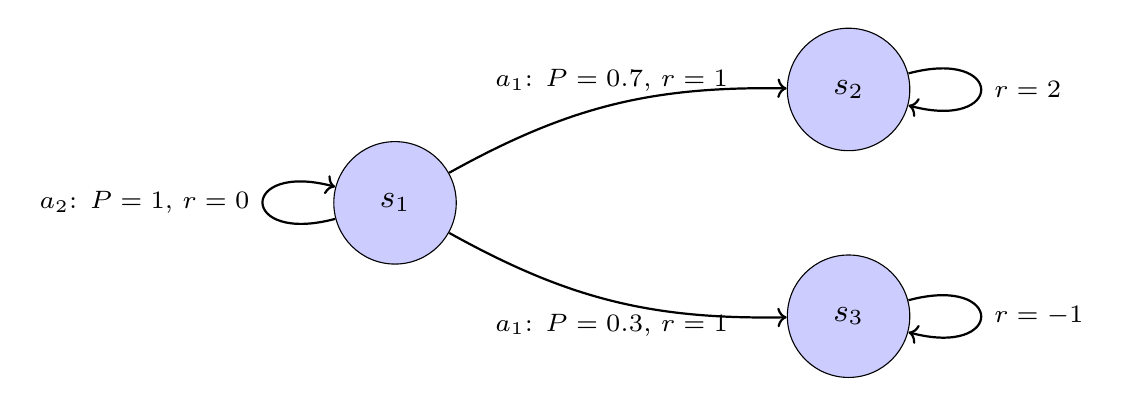
\begin{tikzpicture}[scale=0.9, every node/.style={scale=0.9},
        state/.style={circle, draw, fill=blue!20, minimum size=1.2cm, font=\small},
        action/.style={rectangle, draw, fill=orange!20, minimum width=0.8cm, minimum height=0.6cm, font=\scriptsize}]

        % States
        \node[state] (s1) at (0,0) {$s_1$};
        \node[state] (s2) at (4,1) {$s_2$};
        \node[state] (s3) at (4,-1) {$s_3$};

        % Transitions from s1
        \draw[->, thick, bend left=15] (s1) to node[above, font=\scriptsize] {$a_1$: $P=0.7$, $r=1$} (s2);
        \draw[->, thick, bend right=15] (s1) to node[below, font=\scriptsize] {$a_1$: $P=0.3$, $r=1$} (s3);
        \draw[->, thick] (s1) to[loop left] node[left, font=\scriptsize] {$a_2$: $P=1$, $r=0$} (s1);

        % Self loops
        \draw[->, thick] (s2) to[loop right] node[right, font=\scriptsize] {$r=2$} (s2);
        \draw[->, thick] (s3) to[loop right] node[right, font=\scriptsize] {$r=-1$} (s3);
    \end{tikzpicture}
    \caption{一个简单的 MDP 示例。状态 $s_1$ 有两个动作可选:$a_1$ 以 0.7 概率转移到 $s_2$(高奖励),0.3 概率转移到 $s_3$(负奖励);$a_2$ 原地不动但无奖励。}
    \label{fig:mdp-example}
\end{figure}

\begin{note}
奖励函数的定义有多种形式:
\begin{itemize}
    \item $R(s,a)$:只依赖于当前状态和动作
    \item $R(s,a,s')$:还依赖于下一状态
    \item $R(s)$:只依赖于状态
\end{itemize}
这些形式可以相互转化。例如,$R(s,a,s')$ 可以转化为 $R(s,a) = \sum_{s'} P(s'|s,a) R(s,a,s')$。本书默认使用 $R(s,a)$ 形式。
\end{note}

\subsection{Markov 性质}

MDP 的核心假设是 \textbf{Markov 性质}(Markov Property),也称为"无记忆性":

\begin{definition}[Markov 性质]
\label{def:markov-property}
给定当前状态 $s_t$ 和动作 $a_t$,下一状态 $s_{t+1}$ 和奖励 $r_t$ 的分布只依赖于 $(s_t, a_t)$,与历史状态和动作无关:
\begin{equation}
    P(s_{t+1}, r_t | s_t, a_t) = P(s_{t+1}, r_t | s_0, a_0, s_1, a_1, \ldots, s_t, a_t)
\end{equation}
\end{definition}

直观理解:\textbf{当前状态包含了预测未来所需的所有信息}。历史轨迹可以被"压缩"为当前状态,状态是对历史的"充分统计量"。

\begin{keypoint}
如果真实环境不满足 Markov 性质怎么办?答案是扩展状态表示:
\begin{itemize}
    \item \textbf{历史窗口}:Atari 游戏中用连续 4 帧图像作为状态,捕捉运动信息
    \item \textbf{RNN 隐状态}:用循环神经网络的隐状态编码历史
    \item \textbf{Transformer}:用 attention 机制处理变长历史
\end{itemize}
本质上是把"历史"编码进状态表示里,使得扩展后的状态满足 Markov 性质。
\end{keypoint}

\subsection{状态空间与动作空间的分类}

根据状态空间和动作空间的性质,RL 问题可以分类为:

\begin{table}[H]
    \centering
    \begin{tabular}{@{}lllp{5cm}@{}}
        \toprule
        \textbf{类型} & \textbf{状态空间} & \textbf{动作空间} & \textbf{典型例子} \\
        \midrule
        离散-离散 & 有限/可数 & 有限/可数 & 棋类游戏(棋盘布局 $\times$ 落子位置) \\
        连续-离散 & $\R^n$ & 有限/可数 & Atari 游戏(像素图像 $\times$ 按键) \\
        连续-连续 & $\R^n$ & $\R^m$ & 机器人控制(关节角度 $\times$ 力矩) \\
        \bottomrule
    \end{tabular}
    \caption{RL 问题的分类}
    \label{tab:rl-types}
\end{table}

% ------------------------------------------
\section{轨迹与回报}
\label{sec:trajectory-return}

\subsection{轨迹的定义}

Agent 与环境交互产生的状态-动作-奖励序列称为\textbf{轨迹}(Trajectory),也叫 episode 或 rollout。

\begin{definition}[轨迹]
\label{def:trajectory}
轨迹 $\trajectory$ 是一个状态、动作、奖励的序列:
\begin{equation}
    \trajectory = (s_0, a_0, r_0, s_1, a_1, r_1, \ldots, s_{T-1}, a_{T-1}, r_{T-1}, s_T)
\end{equation}
其中 $T$ 是轨迹的长度(episode 的终止时刻)。
\end{definition}

\begin{figure}[H]
    \centering
    \begin{tikzpicture}[scale=0.85, every node/.style={scale=0.85},
        state/.style={circle, draw, fill=blue!20, minimum size=1.1cm, font=\small},
        action/.style={rectangle, draw, fill=orange!20, minimum size=0.7cm, font=\small}]

        \node[state] (s0) at (0,0) {$s_0$};
        \node[action] (a0) at (2,0) {$a_0$};
        \node[state] (s1) at (4,0) {$s_1$};
        \node[action] (a1) at (6,0) {$a_1$};
        \node[state] (s2) at (8,0) {$s_2$};
        \node[action] (a2) at (10,0) {$a_2$};
        \node at (11.5,0) {$\cdots$};
        \node[state] (sT) at (13,0) {$s_T$};

        % 状态到动作的箭头(策略)
        \draw[->, thick] (s0) -- node[above] {\scriptsize $\policy(a_0|s_0)$} (a0);
        \draw[->, thick] (s1) -- node[above] {\scriptsize $\policy(a_1|s_1)$} (a1);
        \draw[->, thick] (s2) -- node[above] {\scriptsize $\policy(a_2|s_2)$} (a2);

        % 动作到状态的箭头(环境转移),使用 yshift 避免标签重叠
        \draw[->, thick] (a0) -- node[above, yshift=1pt] {\scriptsize $r_0$} node[below, yshift=-8pt] {\scriptsize $P(s_1|s_0,a_0)$} (s1);
        \draw[->, thick] (a1) -- node[above, yshift=1pt] {\scriptsize $r_1$} node[below, yshift=-8pt] {\scriptsize $P(s_2|s_1,a_1)$} (s2);
        \draw[->, thick] (a2) -- node[above] {\scriptsize $r_2$} (11.3,0);
        \draw[->, thick] (11.7,0) -- (sT);

        % Legend - 放在图下方,避免与转移概率标签重叠
        \node[blue!70, font=\footnotesize] at (2, -2.0) {策略决定动作};
        \node[green!50!black, font=\footnotesize] at (7, -2.0) {环境决定转移和奖励};
    \end{tikzpicture}
    \caption{轨迹的生成过程。蓝色圆圈表示状态,橙色方块表示动作。注意两种概率来源:策略 $\policy$ 决定动作,环境 $P$ 决定状态转移。}
    \label{fig:trajectory}
\end{figure}

\subsection{轨迹概率分解}

轨迹的概率如何计算?

\begin{theorem}[轨迹概率分解]
\label{thm:trajectory-prob}
在策略 $\policy$ 下,轨迹 $\trajectory$ 的概率为:
\begin{equation}
    p(\trajectory | \policy) = p(s_0) \prod_{t=0}^{T-1} \policy(a_t | s_t) \cdot P(s_{t+1} | s_t, a_t)
    \label{eq:trajectory-prob}
\end{equation}
\end{theorem}

\begin{proof}
利用条件概率的链式法则和 Markov 性质:
\begin{align}
    p(\trajectory | \policy) &= p(s_0, a_0, s_1, a_1, \ldots, s_T | \policy) \\
    &= p(s_0) \cdot p(a_0 | s_0) \cdot p(s_1 | s_0, a_0) \cdot p(a_1 | s_1) \cdot p(s_2 | s_1, a_1) \cdots \\
    &= p(s_0) \prod_{t=0}^{T-1} \underbrace{p(a_t | s_t)}_{\policy(a_t|s_t)} \cdot \underbrace{p(s_{t+1} | s_t, a_t)}_{P(s_{t+1}|s_t,a_t)}
\end{align}
其中第二步使用了 Markov 性质:$p(s_{t+1} | s_0, a_0, \ldots, s_t, a_t) = p(s_{t+1} | s_t, a_t)$。
\end{proof}

\begin{important}
这个分解非常重要!观察公式 \eqref{eq:trajectory-prob}:
\begin{itemize}
    \item $p(s_0)$:初始状态分布,由环境决定
    \item $\policy(a_t|s_t)$:策略,是我们要学习/优化的对象
    \item $P(s_{t+1}|s_t,a_t)$:环境动力学,由环境决定
\end{itemize}

关键观察:$p(s_0)$ 和 $P(s_{t+1}|s_t,a_t)$ 与策略参数 $\theta$ 无关。因此,当对 $\log p(\trajectory|\policy_\theta)$ 求关于 $\theta$ 的梯度时,环境动力学项会消失!这是 Policy Gradient 定理的核心(见第 \ref{chap:policy-based} 章)。
\end{important}

\subsection{Return(回报)的定义}

\begin{definition}[回报 / Reward-to-go]
\label{def:return}
从时刻 $t$ 开始的\textbf{回报}(Return)或\textbf{Reward-to-go} 定义为未来奖励的折扣累积和:
\begin{equation}
    G_t = \sum_{k=0}^{\infty} \discount^k r_{t+k} = r_t + \discount r_{t+1} + \discount^2 r_{t+2} + \cdots
    \label{eq:return}
\end{equation}
其中 $\discount \in [0,1]$ 是折扣因子。
\end{definition}

回报 $G_t$ 满足一个简单但重要的递推关系:
\begin{equation}
    G_t = r_t + \discount G_{t+1}
    \label{eq:return-recursive}
\end{equation}

Bellman 方程正是基于这个递推结构——下一章将详细展开。

\begin{figure}[H]
    \centering
    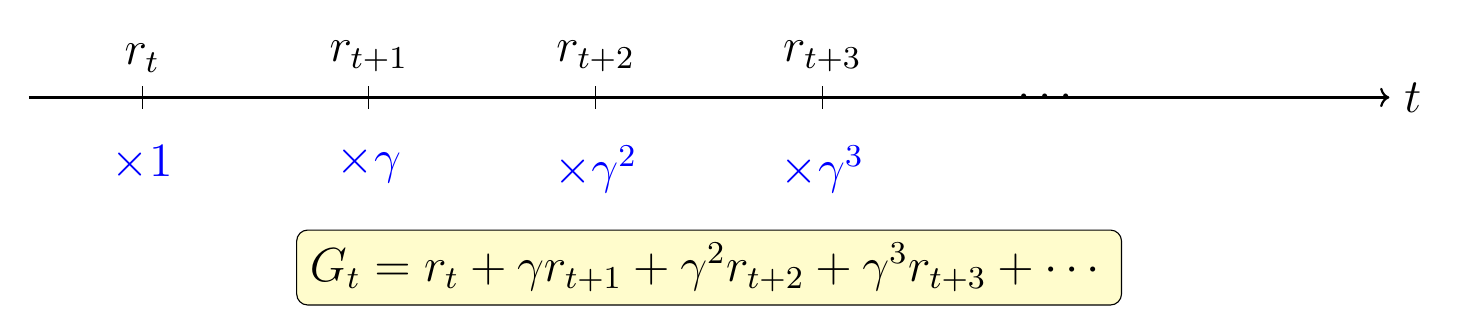
\begin{tikzpicture}[scale=0.9]
        % Timeline
        \draw[->, thick] (0,0) -- (12,0) node[right] {$t$};

        % Rewards
        \foreach \x/\r in {1/$r_t$, 3/$r_{t+1}$, 5/$r_{t+2}$, 7/$r_{t+3}$} {
            \draw (\x, 0.1) -- (\x, -0.1);
            \node[above] at (\x, 0.1) {\r};
        }
        \node at (9, 0) {$\cdots$};

        % Discount factors
        \node[below, blue] at (1, -0.3) {$\times 1$};
        \node[below, blue] at (3, -0.3) {$\times \gamma$};
        \node[below, blue] at (5, -0.3) {$\times \gamma^2$};
        \node[below, blue] at (7, -0.3) {$\times \gamma^3$};

        % G_t
        \node[draw, rounded corners, fill=yellow!20] at (6, -1.5) {$G_t = r_t + \gamma r_{t+1} + \gamma^2 r_{t+2} + \gamma^3 r_{t+3} + \cdots$};
    \end{tikzpicture}
    \caption{回报 $G_t$ 的计算:未来奖励按 $\gamma^k$ 折扣后求和。$\gamma$ 越小,远期奖励的权重越低。}
    \label{fig:return}
\end{figure}

\subsection{Episodic vs Continuing Tasks}

根据任务是否有终止状态,RL 问题分为两类:

\begin{definition}[Episodic 与 Continuing Tasks]\leavevmode
\begin{description}
    \item[Episodic Task] 存在终止状态 $s_T$,轨迹有限长度。例如:棋类游戏(胜负终局)、机器人完成特定任务、一局游戏
    \item[Continuing Task] 没有终止状态,$T \to \infty$。例如:股票交易、持续运行的控制系统、服务器调度
\end{description}
\end{definition}

对于 Continuing Task,必须使用 $\discount < 1$ 以确保回报有界。当 $|r_t| \leq R_{\max}$ 时:
\begin{equation}
    |G_t| \leq \sum_{k=0}^{\infty} \discount^k R_{\max} = \frac{R_{\max}}{1 - \discount}
\end{equation}

\subsection{折扣因子的多重意义}

折扣因子 $\discount$ 是一个看似简单但含义丰富的超参数:

\begin{itemize}
    \item $\discount = 0$:Agent 只关心即时奖励,完全忽略未来("短视")
    \item $\discount = 1$:Agent 平等对待所有未来奖励(仅适用于 Episodic Task)
    \item $0 < \discount < 1$:权衡即时与未来奖励,$\discount$ 越大越"远视"
\end{itemize}

\begin{keypoint}
折扣因子的多重理解:
\begin{enumerate}
    \item \textbf{数学角度}:确保无限和收敛,$G_t$ 有界
    \item \textbf{经济学角度}:时间价值——"现在的 1 元比未来的 1 元更值钱"
    \item \textbf{不确定性角度}:未来越远,预测越不准确,应降低权重
    \item \textbf{实践角度}:$\discount$ 定义了"有效时间尺度"。$1/(1-\discount)$ 步之外的奖励贡献会指数衰减到可以忽略。例如 $\discount=0.99$ 时,有效视野约 100 步。
\end{enumerate}
\end{keypoint}

% ------------------------------------------
\section{策略与价值函数}
\label{sec:policy-value}

\subsection{策略的定义}

\begin{definition}[策略]
\label{def:policy}
\textbf{策略}(Policy)$\policy$ 是从状态到动作的映射,定义了 agent 在每个状态下如何选择动作。策略分为两类:
\begin{itemize}
    \item \textbf{确定性策略}(Deterministic Policy):$\policy: \statespace \to \actionspace$,即 $a = \policy(s)$
    \item \textbf{随机策略}(Stochastic Policy):$\policy: \statespace \times \actionspace \to [0,1]$,即 $\policy(a|s)$ 表示在状态 $s$ 选择动作 $a$ 的概率
\end{itemize}
\end{definition}

随机策略满足归一化条件:对于所有 $s \in \statespace$,
\begin{equation}
    \sum_{a \in \actionspace} \policy(a|s) = 1
\end{equation}

为什么需要随机策略?确定性策略不是更简单吗?

\begin{note}
随机策略的三个优势:
\begin{enumerate}
    \item \textbf{探索}:随机性有助于探索未知动作,避免陷入局部最优
    \item \textbf{对抗性}:在博弈场景中,确定性策略容易被对手预测(想想"石头剪刀布")
    \item \textbf{优化友好}:随机策略的梯度更容易计算(确定性策略的梯度涉及 $\argmax$,不可微)
\end{enumerate}
确定性策略可以看作随机策略的特例(概率集中在单一动作上)。
\end{note}

\subsection{状态价值函数 $\Val^\policy(s)$}

\begin{definition}[状态价值函数]
\label{def:state-value}
策略 $\policy$ 的\textbf{状态价值函数}(State Value Function)定义为从状态 $s$ 出发,遵循策略 $\policy$ 的期望回报:
\begin{equation}
    \Val^\policy(s) = \E_\policy \left[ G_t \mid S_t = s \right] = \E_\policy \left[ \sum_{k=0}^{\infty} \discount^k r_{t+k} \mid S_t = s \right]
    \label{eq:state-value}
\end{equation}
其中期望是对策略 $\policy$ 下产生的所有可能轨迹取的。
\end{definition}

$\Val^\policy(s)$ 回答的问题是:\textbf{在状态 $s$,如果从现在开始一直遵循策略 $\policy$,能获得的期望总奖励是多少?}

\subsection{动作价值函数 $\Qval^\policy(s,a)$}

\begin{definition}[动作价值函数]
\label{def:action-value}
策略 $\policy$ 的\textbf{动作价值函数}(Action Value Function)定义为在状态 $s$ 执行动作 $a$,之后遵循策略 $\policy$ 的期望回报:
\begin{equation}
    \Qval^\policy(s,a) = \E_\policy \left[ G_t \mid S_t = s, A_t = a \right] = \E_\policy \left[ \sum_{k=0}^{\infty} \discount^k r_{t+k} \mid S_t = s, A_t = a \right]
    \label{eq:action-value}
\end{equation}
\end{definition}

$\Qval^\policy(s,a)$ 比 $\Val^\policy(s)$ 提供了更细粒度的信息:它允许我们单独评估每个动作的价值,而不是只知道"按 $\policy$ 走的整体期望"。这使得我们可以比较不同动作的好坏,从而改进策略。

\subsection{$\Val$ 与 $\Qval$ 的关系}

两个价值函数之间存在简单而重要的联系:

\begin{theorem}[$\Val$ 与 $\Qval$ 的关系]
\label{thm:v-q-relation}
\begin{equation}
    \Val^\policy(s) = \sum_{a \in \actionspace} \policy(a|s) \Qval^\policy(s,a) = \E_{a \sim \policy(\cdot|s)} \left[ \Qval^\policy(s,a) \right]
    \label{eq:v-from-q}
\end{equation}
\end{theorem}

\begin{proof}
由全期望公式:
\begin{align}
    \Val^\policy(s) &= \E_\policy \left[ G_t \mid S_t = s \right] \\
    &= \sum_{a \in \actionspace} p(A_t = a | S_t = s) \cdot \E_\policy \left[ G_t \mid S_t = s, A_t = a \right] \\
    &= \sum_{a \in \actionspace} \policy(a|s) \cdot \Qval^\policy(s,a)
\end{align}
\end{proof}

直观理解:状态价值 $\Val^\policy(s)$ 就是所有动作价值 $\Qval^\policy(s,a)$ 按策略概率 $\policy(a|s)$ 加权的平均。

\subsection{优势函数 $\advantage^\policy(s,a)$}

\begin{definition}[优势函数]
\label{def:advantage}
\textbf{优势函数}(Advantage Function)定义为动作价值与状态价值之差:
\begin{equation}
    \advantage^\policy(s,a) = \Qval^\policy(s,a) - \Val^\policy(s)
    \label{eq:advantage}
\end{equation}
\end{definition}

优势函数衡量的是:在状态 $s$ 执行动作 $a$ 相对于"平均水平"(即按策略采样动作)好多少或差多少。

\begin{theorem}[优势函数的关键性质]
\label{thm:advantage-properties}
优势函数在策略分布下的期望为零:
\begin{equation}
    \E_{a \sim \policy(\cdot|s)} \left[ \advantage^\policy(s,a) \right] = 0
\end{equation}
\end{theorem}

\begin{proof}
由公式 \eqref{eq:v-from-q}:
\begin{align}
    \E_{a \sim \policy(\cdot|s)} \left[ \advantage^\policy(s,a) \right]
    &= \E_{a \sim \policy} \left[ \Qval^\policy(s,a) - \Val^\policy(s) \right] \\
    &= \E_{a \sim \policy} \left[ \Qval^\policy(s,a) \right] - \Val^\policy(s) \\
    &= \Val^\policy(s) - \Val^\policy(s) = 0
\end{align}
\end{proof}

\begin{keypoint}
优势函数的直观意义:
\begin{itemize}
    \item $\advantage(s,a) > 0$:动作 $a$ 优于平均水平
    \item $\advantage(s,a) < 0$:动作 $a$ 劣于平均水平
    \item $\advantage(s,a) = 0$:动作 $a$ 与平均水平持平
\end{itemize}
优势函数在 Policy Gradient 中的作用将在第~\ref{chap:policy-based}~章详细讨论。
\end{keypoint}

\subsection{最优策略与最优价值函数}

\begin{definition}[最优价值函数]
\label{def:optimal-value}
\textbf{最优状态价值函数} $\Val^*(s)$ 和\textbf{最优动作价值函数} $\Qval^*(s,a)$ 定义为所有策略中能达到的最大价值:
\begin{align}
    \Val^*(s) &= \max_\policy \Val^\policy(s) \label{eq:optimal-v} \\
    \Qval^*(s,a) &= \max_\policy \Qval^\policy(s,a) \label{eq:optimal-q}
\end{align}
\end{definition}

\begin{definition}[最优策略]
\label{def:optimal-policy}
策略 $\policy^*$ 称为\textbf{最优策略}(Optimal Policy),如果对于所有状态 $s \in \statespace$:
\begin{equation}
    \Val^{\policy^*}(s) = \Val^*(s)
\end{equation}
\end{definition}

\begin{theorem}[最优策略的存在性]
对于有限 MDP(有限状态空间和动作空间),至少存在一个确定性最优策略。
\end{theorem}

最优策略可以由最优动作价值函数直接导出:

\begin{theorem}[从 $\Qval^*$ 导出最优策略]
\label{thm:optimal-policy-from-q}
给定 $\Qval^*$,最优策略为:
\begin{equation}
    \policy^*(s) = \argmax_{a \in \actionspace} \Qval^*(s,a)
    \label{eq:optimal-policy-from-q}
\end{equation}
\end{theorem}

这个结论是 Q-Learning 等 Value-Based 方法的理论基础:\textbf{只要学到 $\Qval^*$,就能直接得到最优策略}。

% ------------------------------------------
\section{RL 问题的形式化目标}
\label{sec:rl-objective}

综合以上定义,强化学习的目标可以形式化为:

\begin{definition}[RL 目标]
\label{def:rl-objective}
找到最优策略 $\policy^*$,使得期望回报最大化:
\begin{equation}
    \policy^* = \argmax_\policy J(\policy)
    \label{eq:rl-objective}
\end{equation}
其中 $J(\policy)$ 是策略的性能指标,常见定义包括:
\begin{enumerate}
    \item \textbf{从固定初始状态出发}:$J(\policy) = \Val^\policy(s_0)$
    \item \textbf{初始状态有分布}:$J(\policy) = \E_{s_0 \sim p(s_0)} \left[ \Val^\policy(s_0) \right]$
    \item \textbf{轨迹期望}:$J(\policy) = \E_{\trajectory \sim \policy} \left[ \sum_{t=0}^{T} \discount^t r_t \right]$
\end{enumerate}
\end{definition}

这三种定义在大多数情况下是等价的。后续章节将介绍解决这一优化问题的不同方法:

\begin{itemize}
    \item \textbf{Value-Based 方法}(第 \ref{chap:value-based} 章):学习 $\Val^*$ 或 $\Qval^*$,再由 $\argmax$ 导出 $\policy^*$
    \item \textbf{Policy-Based 方法}(第 \ref{chap:policy-based} 章):直接优化参数化策略 $\policy_\theta$
    \item \textbf{Actor-Critic 方法}(第 \ref{chap:policy-based} 章):同时学习策略(Actor)和价值函数(Critic)
\end{itemize}

\begin{figure}[H]
    \centering
    \begin{tikzpicture}[scale=0.9, every node/.style={scale=0.9},
        box/.style={draw, rounded corners, minimum width=2.8cm, minimum height=1cm, align=center}]

        \node[box, fill=blue!15] (rl) at (0, 0) {RL 方法};

        \node[box, fill=orange!15] (vb) at (-3.5, -2) {Value-Based\\学习 $\Qval^*$};
        \node[box, fill=green!15] (pb) at (0, -2) {Policy-Based\\学习 $\policy_\theta$};
        \node[box, fill=purple!15] (ac) at (3.5, -2) {Actor-Critic\\学习两者};

        \draw[->, thick] (rl) -- (vb);
        \draw[->, thick] (rl) -- (pb);
        \draw[->, thick] (rl) -- (ac);

        \node[font=\scriptsize, gray] at (-3.5, -3.2) {DQN, Q-Learning};
        \node[font=\scriptsize, gray] at (0, -3.2) {REINFORCE, TRPO};
        \node[font=\scriptsize, gray] at (3.5, -3.2) {A2C, PPO, SAC};
    \end{tikzpicture}
    \caption{RL 方法的三大类别。Value-Based 学习价值函数,Policy-Based 直接学习策略,Actor-Critic 结合两者。}
    \label{fig:rl-methods}
\end{figure}

% ------------------------------------------
\section*{本章小结}

\begin{keypoint}
回顾开篇问题:如何让机器学会序列决策?答案是将问题形式化为 MDP,目标是最大化期望累积奖励。

本章建立的核心概念:
\begin{enumerate}
    \item \textbf{MDP 五元组} $(\statespace, \actionspace, P, R, \discount)$ 是 RL 的标准形式化框架
    \item \textbf{Markov 性质}:当前状态包含预测未来所需的所有信息
    \item \textbf{轨迹概率分解}:$p(\tau|\policy) = p(s_0) \prod_t \policy(a_t|s_t) P(s_{t+1}|s_t,a_t)$,策略与环境动力学分离
    \item \textbf{回报的递推}:$G_t = r_t + \gamma G_{t+1}$,这是 Bellman 方程的起点
    \item \textbf{价值函数}:$\Val^\policy$ 和 $\Qval^\policy$ 衡量策略的长期价值
    \item \textbf{优势函数}:$\advantage^\policy(s,a) = \Qval^\policy(s,a) - \Val^\policy(s)$,期望为零
    \item \textbf{RL 目标}:$\max_\policy J(\policy)$,找到使期望回报最大的策略
\end{enumerate}

下一章将介绍 Bellman 方程——利用回报的递推结构来高效计算价值函数,以及基于价值函数的 Q-Learning、DQN 等算法。
\end{keypoint}



% 第二章:基于价值的强化学习
% ==========================================
% 第二章:基于价值的强化学习
% ==========================================

\chapter{基于价值的强化学习}
\label{chap:value-based}

% ------------------------------------------
\section{引言:从价值到决策}
\label{sec:value-intro}

\subsection{核心问题}

在第一章中,我们定义了价值函数 $\Val^\policy(s)$ 和 $\Qval^\policy(s,a)$,它们衡量了给定策略 $\policy$ 下状态或状态-动作对的"好坏"。现在自然的问题是:

\begin{quote}
\textbf{如何计算价值函数?如何从价值函数导出最优策略?}
\end{quote}

这两个问题的答案构成了 Value-Based RL 的核心。本章将介绍三类方法:
\begin{enumerate}
    \item \textbf{动态规划}(Dynamic Programming):当环境模型已知时,精确求解
    \item \textbf{无模型估计}(MC 与 TD):当环境模型未知时,从采样中学习
    \item \textbf{深度 Q 网络}(DQN):处理大规模或连续状态空间
\end{enumerate}

\subsection{为什么要学习价值函数?}

一个核心观察是:\textbf{如果我们知道最优动作价值函数 $\Qval^*(s,a)$,就能直接导出最优策略}:
\begin{equation}
    \policy^*(s) = \argmax_a \Qval^*(s,a)
\end{equation}

这是 Value-Based 方法的理论基础——不直接学习策略,而是通过学习价值函数间接得到策略。

\begin{figure}[H]
    \centering
    \begin{tikzpicture}[
        box/.style={draw, rounded corners, fill=blue!10, minimum width=2.5cm, minimum height=1cm, align=center},
        arrow/.style={->, thick, >=stealth}
    ]
        % Boxes
        \node[box, fill=orange!20] (value) at (0,0) {价值函数\\$\Val^*$ 或 $\Qval^*$};
        \node[box, fill=green!20] (policy) at (5,0) {最优策略\\$\policy^*$};
        \node[box] (method) at (0,-2) {Value-Based\\方法};

        % Arrows
        \draw[arrow] (value) -- node[above] {$\argmax$} (policy);
        \draw[arrow] (method) -- (value);

        % Labels
        \node[text width=3cm, align=center, font=\footnotesize] at (-3,-2) {DP, MC, TD\\Q-Learning, DQN};
    \end{tikzpicture}
    \caption{Value-Based RL 的核心思路:学习价值函数,通过 $\argmax$ 导出策略}
    \label{fig:value-based-idea}
\end{figure}

% ------------------------------------------
\section{Bellman 方程}
\label{sec:bellman}

Bellman 方程是 RL 的核心方程,它揭示了价值函数的递推结构。理解 Bellman 方程是掌握所有 Value-Based 方法的基础。

\subsection{直觉:一步分解}

Bellman 方程的核心形式是:
\begin{equation}
    \Val^\policy(s) = \E \left[ r + \discount \Val^\policy(s') \right]
    \label{eq:bellman-intuition}
\end{equation}
用文字说:\textbf{当前状态的价值 = 即时奖励 + 折扣后的下一状态价值}。

这个递推关系使得我们可以通过迭代来计算价值函数,而不需要枚举所有可能的轨迹。

\begin{figure}[H]
    \centering
    \begin{tikzpicture}[scale=0.85]
        % Timeline
        \draw[->, thick] (0,0) -- (10,0) node[right] {时间};

        % Points
        \foreach \x/\label in {1/$t$, 4/$t+1$, 7/$t+2$} {
            \fill (\x, 0) circle (2pt);
            \node[below] at (\x, -0.2) {\label};
        }

        % Current value
        \draw[decorate, decoration={brace, amplitude=10pt, raise=5pt}] (1,0) -- (9,0)
            node[midway, above=15pt] {$\Val^\policy(s_t) = \E[G_t]$};

        % Decomposition
        \draw[decorate, decoration={brace, amplitude=8pt, raise=5pt, mirror}] (1,-0.5) -- (4,-0.5)
            node[midway, below=12pt] {$r_t$};
        \draw[decorate, decoration={brace, amplitude=8pt, raise=5pt, mirror}] (4,-0.5) -- (9,-0.5)
            node[midway, below=12pt] {$\discount \Val^\policy(s_{t+1})$};
    \end{tikzpicture}
    \caption{Bellman 方程的直觉:将无限长的回报分解为"一步奖励 + 剩余价值"}
    \label{fig:bellman-intuition}
\end{figure}

\subsection{Bellman Expectation Equation 的详细推导}

我们首先推导策略 $\policy$ 下的 Bellman Expectation Equation。

\begin{theorem}[Bellman Expectation Equation for $\Val^\policy$]
\label{thm:bellman-expectation-v}
对于任意策略 $\policy$,状态价值函数满足:
\begin{equation}
    \Val^\policy(s) = \sum_{a \in \actionspace} \policy(a|s) \left[ R(s,a) + \discount \sum_{s' \in \statespace} P(s'|s,a) \Val^\policy(s') \right]
    \label{eq:bellman-expectation-v}
\end{equation}
或写成紧凑的期望形式:
\begin{equation}
    \Val^\policy(s) = \E_{a \sim \policy, s' \sim P} \left[ R(s,a) + \discount \Val^\policy(s') \mid S_t = s \right]
\end{equation}
\end{theorem}

\begin{proof}
从状态价值函数的定义出发(回顾第一章 \eqref{eq:state-value}):
\begin{align}
    \Val^\policy(s) &= \E_\policy \left[ G_t \mid S_t = s \right] \\
    &= \E_\policy \left[ r_t + \discount G_{t+1} \mid S_t = s \right] \quad \text{(回报的递推关系 \eqref{eq:return-recursive})}
\end{align}

关键步骤:由于 $G_{t+1}$ 只依赖于 $S_{t+1}$ 之后的轨迹,我们可以条件分解:
\begin{align}
    \Val^\policy(s) &= \E_\policy \left[ r_t + \discount \E_\policy[G_{t+1} | S_{t+1}] \mid S_t = s \right] \\
    &= \E_\policy \left[ r_t + \discount \Val^\policy(S_{t+1}) \mid S_t = s \right]
\end{align}

其中最后一步使用了 $\Val^\policy(s') = \E_\policy[G_{t+1}|S_{t+1}=s']$ 的定义。

现在展开期望。由于给定 $S_t = s$:
\begin{itemize}
    \item 动作 $A_t = a$ 的概率为 $\policy(a|s)$
    \item 给定 $(s, a)$,下一状态 $S_{t+1} = s'$ 的概率为 $P(s'|s,a)$
    \item 即时奖励 $r_t = R(s,a)$(假设确定性奖励,随机情况类似)
\end{itemize}

因此:
\begin{align}
    \Val^\policy(s) &= \sum_{a \in \actionspace} \policy(a|s) \sum_{s' \in \statespace} P(s'|s,a) \left[ R(s,a) + \discount \Val^\policy(s') \right] \\
    &= \sum_{a \in \actionspace} \policy(a|s) \left[ R(s,a) + \discount \sum_{s' \in \statespace} P(s'|s,a) \Val^\policy(s') \right]
\end{align}
\end{proof}

\begin{figure}[H]
    \centering
    \begin{tikzpicture}[scale=0.9, every node/.style={scale=0.9}]
        % State s (root)
        \node[circle, draw, fill=blue!25, minimum size=1.4cm, font=\bfseries] (s) at (0,0) {$s$};
        \node[above=0.4cm of s, font=\small] {$\Val^\policy(s)$};

        % Actions (level 1)
        \node[rectangle, draw, fill=orange!25, minimum size=0.8cm] (a1) at (-3,-2) {$a_1$};
        \node[rectangle, draw, fill=orange!25, minimum size=0.8cm] (a2) at (0,-2) {$a_2$};
        \node[rectangle, draw, fill=orange!25, minimum size=0.8cm] (a3) at (3,-2) {$a_3$};

        % Policy probabilities
        \draw[->, thick, blue!70] (s) -- node[left, pos=0.6, font=\scriptsize] {$\policy(a_1|s)$} (a1);
        \draw[->, thick, blue!70] (s) -- node[right, pos=0.4, font=\scriptsize] {$\policy(a_2|s)$} (a2);
        \draw[->, thick, blue!70] (s) -- node[right, pos=0.6, font=\scriptsize] {$\policy(a_3|s)$} (a3);

        % Next states (level 2)
        \node[circle, draw, fill=blue!15, minimum size=1cm] (s11) at (-4,-4.5) {$s'_1$};
        \node[circle, draw, fill=blue!15, minimum size=1cm] (s12) at (-2,-4.5) {$s'_2$};
        \node[circle, draw, fill=blue!15, minimum size=1cm] (s21) at (-0.5,-4.5) {$s'_1$};
        \node[circle, draw, fill=blue!15, minimum size=1cm] (s22) at (1.5,-4.5) {$s'_3$};
        \node[circle, draw, fill=blue!15, minimum size=1cm] (s31) at (3,-4.5) {$s'_2$};

        % Transition probabilities and rewards
        \draw[->, dashed, gray] (a1) -- node[left, font=\tiny] {$P, R$} (s11);
        \draw[->, dashed, gray] (a1) -- node[right, font=\tiny] {$P, R$} (s12);
        \draw[->, dashed, gray] (a2) -- node[left, font=\tiny] {$P, R$} (s21);
        \draw[->, dashed, gray] (a2) -- node[right, font=\tiny] {$P, R$} (s22);
        \draw[->, dashed, gray] (a3) -- node[right, font=\tiny] {$P, R$} (s31);

        % Value labels
        \node[below=0.2cm of s11, font=\tiny] {$\discount\Val^\policy(s'_1)$};
        \node[below=0.2cm of s12, font=\tiny] {$\discount\Val^\policy(s'_2)$};

        % Legend
        \node[draw, rounded corners, fill=gray!10, font=\scriptsize, text width=4cm] at (6, -2) {
            \textbf{Backup 图说明}\\
            $\circ$ = 状态节点\\
            $\square$ = 动作节点\\
            蓝色箭头 = 策略 $\policy(a|s)$\\
            灰色虚线 = 环境转移 $P(s'|s,a)$
        };
    \end{tikzpicture}
    \caption{Bellman Expectation Equation 的 Backup 图。从状态 $s$ 出发,先按策略 $\policy(a|s)$ 选择动作,再按环境转移概率 $P(s'|s,a)$ 到达下一状态。价值"回溯"地从叶子节点传播到根节点。}
    \label{fig:bellman-backup}
\end{figure}

类似地,我们可以推导 $\Qval^\policy$ 的 Bellman Expectation Equation:

\begin{theorem}[Bellman Expectation Equation for $\Qval^\policy$]
\label{thm:bellman-expectation-q}
对于任意策略 $\policy$,动作价值函数满足:
\begin{equation}
    \Qval^\policy(s,a) = R(s,a) + \discount \sum_{s' \in \statespace} P(s'|s,a) \sum_{a' \in \actionspace} \policy(a'|s') \Qval^\policy(s',a')
    \label{eq:bellman-expectation-q}
\end{equation}
或写成期望形式:
\begin{equation}
    \Qval^\policy(s,a) = R(s,a) + \discount \E_{s' \sim P, a' \sim \policy} \left[ \Qval^\policy(s', a') \right]
\end{equation}
\end{theorem}

\begin{proof}
从动作价值函数的定义出发:
\begin{align}
    \Qval^\policy(s,a) &= \E_\policy \left[ G_t \mid S_t = s, A_t = a \right] \\
    &= \E_\policy \left[ r_t + \discount G_{t+1} \mid S_t = s, A_t = a \right] \\
    &= R(s,a) + \discount \E_\policy \left[ G_{t+1} \mid S_t = s, A_t = a \right]
\end{align}

关键步骤:由 Markov 性质,给定 $(s,a)$ 后,$G_{t+1}$ 只通过 $S_{t+1}$ 影响。对 $S_{t+1}$ 的分布求期望:
\begin{align}
    \E_\policy \left[ G_{t+1} \mid S_t = s, A_t = a \right] &= \sum_{s'} P(s'|s,a) \E_\policy \left[ G_{t+1} \mid S_{t+1} = s' \right] \\
    &= \sum_{s'} P(s'|s,a) \Val^\policy(s')
\end{align}

利用第一章的 V-Q 关系 $\Val^\policy(s') = \sum_{a'} \policy(a'|s') \Qval^\policy(s',a')$,代入得:
\begin{equation}
    \Qval^\policy(s,a) = R(s,a) + \discount \sum_{s'} P(s'|s,a) \sum_{a'} \policy(a'|s') \Qval^\policy(s',a')
\end{equation}
\end{proof}

\begin{keypoint}
$\Val^\policy$ 与 $\Qval^\policy$ 的相互表示是推导 Bellman 方程的关键:
\begin{align}
    \Val^\policy(s) &= \sum_{a} \policy(a|s) \Qval^\policy(s,a) \label{eq:v-from-q-2} \\
    \Qval^\policy(s,a) &= R(s,a) + \discount \sum_{s'} P(s'|s,a) \Val^\policy(s') \label{eq:q-from-v}
\end{align}
将 \eqref{eq:q-from-v} 代入 \eqref{eq:v-from-q-2} 得到 $\Val^\policy$ 的 Bellman 方程;将 \eqref{eq:v-from-q-2} 代入 \eqref{eq:q-from-v} 得到 $\Qval^\policy$ 的 Bellman 方程。
\end{keypoint}

\subsection{Bellman Optimality Equation 的详细推导}

最优价值函数满足 Bellman Optimality Equation。与 Expectation 版本不同,这里对动作求\textbf{最大值}而非期望。

\begin{theorem}[Bellman Optimality Equation for $\Val^*$]
\label{thm:bellman-optimality-v}
最优状态价值函数满足:
\begin{equation}
    \Val^*(s) = \max_{a \in \actionspace} \left[ R(s,a) + \discount \sum_{s' \in \statespace} P(s'|s,a) \Val^*(s') \right]
    \label{eq:bellman-optimality-v}
\end{equation}
\end{theorem}

\begin{proof}
最优价值函数的定义是所有策略中最大的价值:
\begin{equation}
    \Val^*(s) = \max_\policy \Val^\policy(s)
\end{equation}

最优策略 $\policy^*$ 是确定性的,在每个状态选择使 $\Qval^*(s,a)$ 最大的动作。因此:
\begin{align}
    \Val^*(s) &= \Val^{\policy^*}(s) \\
    &= \max_a \Qval^*(s,a) \quad \text{(最优策略选择最大 Q 值的动作)}
\end{align}

由 \eqref{eq:q-from-v} 对最优策略成立:
\begin{equation}
    \Qval^*(s,a) = R(s,a) + \discount \sum_{s'} P(s'|s,a) \Val^*(s')
\end{equation}

代入得:
\begin{equation}
    \Val^*(s) = \max_a \left[ R(s,a) + \discount \sum_{s'} P(s'|s,a) \Val^*(s') \right]
\end{equation}
\end{proof}

\begin{theorem}[Bellman Optimality Equation for $\Qval^*$]
\label{thm:bellman-optimality-q}
最优动作价值函数满足:
\begin{equation}
    \Qval^*(s,a) = R(s,a) + \discount \sum_{s' \in \statespace} P(s'|s,a) \max_{a' \in \actionspace} \Qval^*(s',a')
    \label{eq:bellman-optimality-q}
\end{equation}
\end{theorem}

\begin{proof}
\begin{align}
    \Qval^*(s,a) &= R(s,a) + \discount \sum_{s'} P(s'|s,a) \Val^*(s') \\
    &= R(s,a) + \discount \sum_{s'} P(s'|s,a) \max_{a'} \Qval^*(s',a')
\end{align}
其中最后一步使用了 $\Val^*(s') = \max_{a'} \Qval^*(s',a')$。
\end{proof}

\begin{figure}[H]
    \centering
    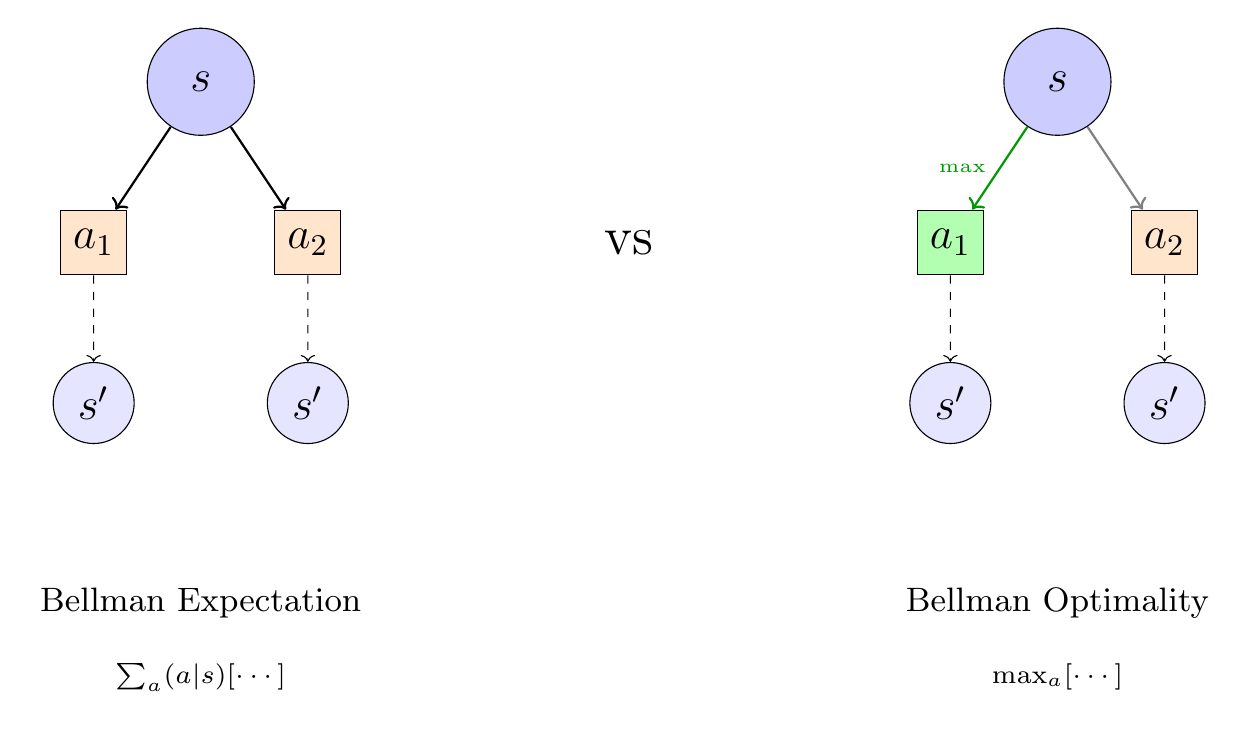
\begin{tikzpicture}[scale=0.85]
        % Bellman Expectation
        \begin{scope}[shift={(-4,0)}]
            \node[circle, draw, fill=blue!20, minimum size=1cm] (s1) at (0,0) {$s$};
            \node[rectangle, draw, fill=orange!20, minimum size=0.6cm] (a11) at (-1,-1.5) {$a_1$};
            \node[rectangle, draw, fill=orange!20, minimum size=0.6cm] (a12) at (1,-1.5) {$a_2$};
            \draw[->, thick] (s1) -- node[left, font=\tiny] {$\policy$} (a11);
            \draw[->, thick] (s1) -- node[right, font=\tiny] {$\policy$} (a12);
            \node[circle, draw, fill=blue!10, minimum size=0.7cm] (s11) at (-1,-3) {$s'$};
            \node[circle, draw, fill=blue!10, minimum size=0.7cm] (s12) at (1,-3) {$s'$};
            \draw[->, dashed] (a11) -- (s11);
            \draw[->, dashed] (a12) -- (s12);
            \node[below=0.3cm of s1, yshift=-3.8cm, font=\small] {Bellman Expectation};
            \node[below=0.3cm of s1, yshift=-4.5cm, font=\scriptsize] {$\sum_a \policy(a|s) [\cdots]$};
        \end{scope}

        % Bellman Optimality
        \begin{scope}[shift={(4,0)}]
            \node[circle, draw, fill=blue!20, minimum size=1cm] (s2) at (0,0) {$s$};
            \node[rectangle, draw, fill=green!30, minimum size=0.6cm] (a21) at (-1,-1.5) {$a_1$};
            \node[rectangle, draw, fill=orange!20, minimum size=0.6cm] (a22) at (1,-1.5) {$a_2$};
            \draw[->, thick, green!60!black] (s2) -- node[left, font=\tiny] {$\max$} (a21);
            \draw[->, thick, gray] (s2) -- (a22);
            \node[circle, draw, fill=blue!10, minimum size=0.7cm] (s21) at (-1,-3) {$s'$};
            \node[circle, draw, fill=blue!10, minimum size=0.7cm] (s22) at (1,-3) {$s'$};
            \draw[->, dashed] (a21) -- (s21);
            \draw[->, dashed] (a22) -- (s22);
            \node[below=0.3cm of s2, yshift=-3.8cm, font=\small] {Bellman Optimality};
            \node[below=0.3cm of s2, yshift=-4.5cm, font=\scriptsize] {$\max_a [\cdots]$};
        \end{scope}

        % VS
        \node[font=\Large] at (0, -1.5) {vs};
    \end{tikzpicture}
    \caption{Bellman Expectation vs. Bellman Optimality。左图对动作求加权平均(按 $\policy$),右图对动作求最大值。}
    \label{fig:bellman-comparison}
\end{figure}

\begin{important}
Bellman Expectation vs. Bellman Optimality 的关键区别:
\begin{itemize}
    \item \textbf{Bellman Expectation}:对动作求加权平均(按 $\policy(a|s)$),描述\textbf{给定策略}的价值
    \item \textbf{Bellman Optimality}:对动作求最大值($\max_a$),描述\textbf{最优策略}的价值
\end{itemize}
\textbf{Q-Learning 直接逼近 $\Qval^*$,因此使用 Bellman Optimality Equation 作为更新目标}。
\end{important}

\subsection{$\Val^*$ 与 $\Qval^*$ 的关系}

最优价值函数之间的关系:
\begin{align}
    \Val^*(s) &= \max_a \Qval^*(s,a) \\
    \Qval^*(s,a) &= R(s,a) + \discount \sum_{s'} P(s'|s,a) \Val^*(s')
\end{align}

由 $\Qval^*$ 可以直接导出最优策略:
\begin{equation}
    \policy^*(s) = \argmax_a \Qval^*(s,a)
\end{equation}

这是 Q-Learning 系列方法的理论基础:\textbf{只要学到 $\Qval^*$,就能得到最优策略}。

\subsection{Bellman 算子与收缩性质}

为了理解为什么基于 Bellman 方程的迭代方法能够收敛,我们引入 Bellman 算子的概念。

\begin{definition}[Bellman 算子]
定义 Bellman Expectation 算子 $\mathcal{T}^\policy$ 和 Bellman Optimality 算子 $\mathcal{T}^*$:
\begin{align}
    (\mathcal{T}^\policy \Val)(s) &= \sum_a \policy(a|s) \left[ R(s,a) + \discount \sum_{s'} P(s'|s,a) \Val(s') \right] \\
    (\mathcal{T}^* \Val)(s) &= \max_a \left[ R(s,a) + \discount \sum_{s'} P(s'|s,a) \Val(s') \right]
\end{align}
\end{definition}

\begin{theorem}[Bellman 算子的收缩性]
\label{thm:bellman-contraction}
Bellman 算子是 $\gamma$-收缩映射。即对于任意两个价值函数 $\Val_1, \Val_2$:
\begin{equation}
    \| \mathcal{T}^\policy \Val_1 - \mathcal{T}^\policy \Val_2 \|_\infty \leq \discount \| \Val_1 - \Val_2 \|_\infty
\end{equation}
$\mathcal{T}^*$ 同样满足此性质。
\end{theorem}

\begin{proof}
对于任意状态 $s$:
\begin{align}
    |(\mathcal{T}^\policy \Val_1)(s) - (\mathcal{T}^\policy \Val_2)(s)| &= \left| \discount \sum_a \policy(a|s) \sum_{s'} P(s'|s,a) [\Val_1(s') - \Val_2(s')] \right| \\
    &\leq \discount \sum_a \policy(a|s) \sum_{s'} P(s'|s,a) |\Val_1(s') - \Val_2(s')| \\
    &\leq \discount \| \Val_1 - \Val_2 \|_\infty \underbrace{\sum_a \policy(a|s) \sum_{s'} P(s'|s,a)}_{=1} \\
    &= \discount \| \Val_1 - \Val_2 \|_\infty
\end{align}
对所有 $s$ 取最大,得到结论。
\end{proof}

\begin{keypoint}
收缩性质的重要推论:
\begin{enumerate}
    \item \textbf{唯一不动点}:Bellman 算子有唯一的不动点 $\Val^\policy$(或 $\Val^*$)
    \item \textbf{迭代收敛}:从任意初始 $\Val_0$ 出发,$\Val_{k+1} = \mathcal{T}\Val_k$ 收敛到不动点
    \item \textbf{收敛速度}:误差以 $\discount^k$ 的速度指数衰减
\end{enumerate}
\end{keypoint}

% ------------------------------------------
\section{动态规划方法}
\label{sec:dp}

当环境模型 $P(s'|s,a)$ 和 $R(s,a)$ 完全已知时,可以使用动态规划(Dynamic Programming, DP)方法精确求解最优策略。

\subsection{Policy Evaluation(策略评估)}

给定策略 $\policy$,如何计算其价值函数 $\Val^\policy$?

\begin{definition}[Policy Evaluation]
Policy Evaluation 是通过迭代 Bellman Expectation 方程来计算 $\Val^\policy$ 的过程:
\begin{equation}
    \Val_{k+1}(s) = \sum_a \policy(a|s) \left[ R(s,a) + \discount \sum_{s'} P(s'|s,a) \Val_k(s') \right]
    \label{eq:policy-eval-update}
\end{equation}
从任意初始 $\Val_0$ 开始,迭代直到收敛 $\Val_k \to \Val^\policy$。
\end{definition}

\begin{theorem}[Policy Evaluation 的收敛性]
\label{thm:policy-eval-convergence}
对于任意初始 $\Val_0$ 和 $\discount < 1$,Policy Evaluation 迭代收敛到唯一的 $\Val^\policy$。收敛速度为 $O(\discount^k)$。
\end{theorem}

\begin{proof}
由定理 \ref{thm:bellman-contraction},Bellman 算子 $\mathcal{T}^\policy$ 是 $\gamma$-收缩映射。由 Banach 不动点定理:
\begin{enumerate}
    \item 存在唯一不动点 $\Val^\policy$ 使得 $\mathcal{T}^\policy \Val^\policy = \Val^\policy$
    \item 对任意 $\Val_0$,序列 $\Val_{k+1} = \mathcal{T}^\policy \Val_k$ 收敛到 $\Val^\policy$
\end{enumerate}

误差界:$\|\Val_k - \Val^\policy\|_\infty \leq \discount^k \|\Val_0 - \Val^\policy\|_\infty$
\end{proof}

\begin{algorithm}[H]
\caption{Policy Evaluation}
\label{alg:policy-evaluation}
\KwInput{策略 $\policy$,MDP $(\statespace, \actionspace, P, R, \discount)$,收敛阈值 $\theta$}
\KwOutput{价值函数 $\Val^\policy$}
初始化 $\Val(s) = 0$ 对于所有 $s \in \statespace$\;
\Repeat{$\Delta < \theta$}{
    $\Delta \leftarrow 0$\;
    \ForEach{$s \in \statespace$}{
        $v \leftarrow \Val(s)$\;
        $\Val(s) \leftarrow \sum_a \policy(a|s) \left[ R(s,a) + \discount \sum_{s'} P(s'|s,a) \Val(s') \right]$\;
        $\Delta \leftarrow \max(\Delta, |v - \Val(s)|)$\;
    }
}
\Return{$\Val$}
\end{algorithm}

\subsection{Policy Improvement(策略改进)}

给定 $\Val^\policy$,如何构造一个更好的策略?

\begin{theorem}[Policy Improvement Theorem]
\label{thm:policy-improvement}
设 $\policy$ 和 $\policy'$ 是两个策略。如果对于所有 $s \in \statespace$:
\begin{equation}
    \Qval^\policy(s, \policy'(s)) \geq \Val^\policy(s)
    \label{eq:policy-improvement-condition}
\end{equation}
则 $\policy'$ 至少与 $\policy$ 一样好:对于所有 $s$,$\Val^{\policy'}(s) \geq \Val^\policy(s)$。
\end{theorem}

\begin{proof}
从条件 \eqref{eq:policy-improvement-condition} 出发,利用 $\Qval^\policy$ 的定义展开:
\begin{align}
    \Val^\policy(s) &\leq \Qval^\policy(s, \policy'(s)) \\
    &= R(s, \policy'(s)) + \discount \sum_{s'} P(s'|s, \policy'(s)) \Val^\policy(s') \\
    &\leq R(s, \policy'(s)) + \discount \sum_{s'} P(s'|s, \policy'(s)) \Qval^\policy(s', \policy'(s')) \quad \text{(再用条件)}\\
    &= R(s, \policy'(s)) + \discount \sum_{s'} P(s'|s, \policy'(s)) \left[ R(s', \policy'(s')) + \discount \sum_{s''} P(s''|s', \policy'(s')) \Val^\policy(s'') \right]
\end{align}

继续展开,直到 episode 结束(或利用折扣因子使尾部趋近于零):
\begin{align}
    \Val^\policy(s) &\leq \E_{\policy'} \left[ r_0 + \discount r_1 + \discount^2 r_2 + \cdots \mid S_0 = s \right] \\
    &= \Val^{\policy'}(s)
\end{align}
\end{proof}

\begin{note}
Policy Improvement Theorem 的直觉:如果在每个状态,按 $\policy'$ 选择动作比按 $\policy$ 选择更好(体现在 Q 值上),那么整体策略 $\policy'$ 也更好。
\end{note}

贪心策略改进保证了条件 \eqref{eq:policy-improvement-condition} 以等号或严格大于成立:

\begin{definition}[贪心策略改进]
给定 $\Val^\policy$,定义贪心改进策略:
\begin{equation}
    \policy'(s) = \argmax_a \Qval^\policy(s,a) = \argmax_a \left[ R(s,a) + \discount \sum_{s'} P(s'|s,a) \Val^\policy(s') \right]
    \label{eq:greedy-improvement}
\end{equation}
\end{definition}

对于贪心改进:
\begin{equation}
    \Qval^\policy(s, \policy'(s)) = \max_a \Qval^\policy(s, a) \geq \Qval^\policy(s, \policy(s)) = \Val^\policy(s)
\end{equation}
因此满足 Policy Improvement Theorem 的条件。

\subsection{Policy Iteration}

交替进行 Policy Evaluation 和 Policy Improvement:

\begin{figure}[H]
    \centering
    \begin{tikzpicture}[
        box/.style={draw, rounded corners, fill=blue!15, minimum width=2cm, minimum height=0.8cm, align=center},
        arrow/.style={->, thick, >=stealth}
    ]
        % Boxes
        \node[box] (pi1) at (0,0) {$\policy_0$};
        \node[box, fill=green!15] (v1) at (2.5,0) {$\Val^{\policy_0}$};
        \node[box] (pi2) at (5,0) {$\policy_1$};
        \node[box, fill=green!15] (v2) at (7.5,0) {$\Val^{\policy_1}$};
        \node[box] (pi3) at (10,0) {$\policy_2$};
        \node at (11.5, 0) {$\cdots$};

        % Arrows - 使用 yshift 上移标签避免被节点遮挡
        \draw[arrow] (pi1) -- node[above, font=\scriptsize, yshift=6pt] {Eval} (v1);
        \draw[arrow] (v1) -- node[above, font=\scriptsize, yshift=6pt] {Improve} (pi2);
        \draw[arrow] (pi2) -- node[above, font=\scriptsize, yshift=6pt] {Eval} (v2);
        \draw[arrow] (v2) -- node[above, font=\scriptsize, yshift=6pt] {Improve} (pi3);

        % Labels
        \node[below=0.5cm of v1, font=\small, text=gray] {完整求解};
        \node[below=0.5cm of pi2, font=\small, text=gray] {贪心};
    \end{tikzpicture}
    \caption{Policy Iteration 的流程:评估 $\to$ 改进 $\to$ 评估 $\to$ 改进 $\to$ $\cdots$}
    \label{fig:policy-iteration}
\end{figure}

\begin{algorithm}[H]
\caption{Policy Iteration}
\label{alg:policy-iteration}
\KwInput{MDP $(\statespace, \actionspace, P, R, \discount)$}
\KwOutput{最优策略 $\policy^*$ 和最优价值 $\Val^*$}
初始化 $\policy$ 为任意策略\;
\Repeat{$\policy$ 不再改变(policy-stable = true)}{
    \textbf{Policy Evaluation}: 计算 $\Val^\policy$(使用算法 \ref{alg:policy-evaluation})\;
    policy-stable $\leftarrow$ true\;
    \ForEach{$s \in \statespace$}{
        old-action $\leftarrow \policy(s)$\;
        $\policy(s) \leftarrow \argmax_a \left[ R(s,a) + \discount \sum_{s'} P(s'|s,a) \Val^\policy(s') \right]$\;
        \If{old-action $\neq \policy(s)$}{
            policy-stable $\leftarrow$ false\;
        }
    }
}
\Return{$\policy, \Val^\policy$}
\end{algorithm}

\begin{theorem}[Policy Iteration 的有限步收敛]
对于有限 MDP,Policy Iteration 在有限步内收敛到最优策略 $\policy^*$。
\end{theorem}

\begin{proof}
\begin{enumerate}
    \item 由 Policy Improvement Theorem,每次迭代 $\Val^{\policy_{k+1}}(s) \geq \Val^{\policy_k}(s)$ 对所有 $s$ 成立
    \item 有限 MDP 只有有限多个确定性策略($|\actionspace|^{|\statespace|}$ 个)
    \item 价值函数严格单调递增(除非已是最优),因此不会循环
    \item 结合上述,必在有限步内收敛
\end{enumerate}
\end{proof}

\subsection{Value Iteration}

Value Iteration 将 Policy Evaluation 和 Policy Improvement 合并为一步,直接迭代 Bellman Optimality 方程:

\begin{algorithm}[H]
\caption{Value Iteration}
\label{alg:value-iteration}
\KwInput{MDP $(\statespace, \actionspace, P, R, \discount)$, 收敛阈值 $\theta$}
\KwOutput{最优价值 $\Val^*$ 和最优策略 $\policy^*$}
初始化 $\Val(s) = 0$ 对于所有 $s$\;
\Repeat{$\Delta < \theta$}{
    $\Delta \leftarrow 0$\;
    \ForEach{$s \in \statespace$}{
        $v \leftarrow \Val(s)$\;
        $\Val(s) \leftarrow \max_a \left[ R(s,a) + \discount \sum_{s'} P(s'|s,a) \Val(s') \right]$\;
        $\Delta \leftarrow \max(\Delta, |v - \Val(s)|)$\;
    }
}
$\policy^*(s) \leftarrow \argmax_a \left[ R(s,a) + \discount \sum_{s'} P(s'|s,a) \Val(s') \right]$ 对于所有 $s$\;
\Return{$\Val, \policy^*$}
\end{algorithm}

\begin{keypoint}
Value Iteration vs. Policy Iteration 的对比:

\begin{table}[H]
    \centering
    \begin{tabular}{@{}lcc@{}}
        \toprule
        & \textbf{Policy Iteration} & \textbf{Value Iteration} \\
        \midrule
        Policy Evaluation & 完整求解 $\Val^\policy$ & 仅一步 Bellman 更新 \\
        理论依据 & Bellman Expectation & Bellman Optimality \\
        每轮复杂度 & 高(需多次内循环) & 低(单次遍历) \\
        收敛轮数 & 少 & 多 \\
        总体效率 & 较低 & 通常更高 \\
        \bottomrule
    \end{tabular}
\end{table}

实践中,Value Iteration 通常更高效,因为不需要在每轮完整求解 $\Val^\policy$。
\end{keypoint}

\subsection{DP 方法的局限性}

动态规划虽然能精确求解,但有明显局限:
\begin{enumerate}
    \item \textbf{需要完整模型}:必须知道 $P(s'|s,a)$ 和 $R(s,a)$
    \item \textbf{状态空间遍历}:每轮需要遍历所有状态,复杂度 $O(|\statespace|^2 |\actionspace|)$
    \item \textbf{无法处理连续空间}:表格方法无法直接应用
\end{enumerate}

这些局限促使了无模型方法(MC、TD)和函数逼近方法(DQN)的发展。

% ------------------------------------------
\section{无模型方法:Monte Carlo vs Temporal Difference}
\label{sec:mc-td}

当环境模型未知时,需要通过与环境交互的样本来估计价值函数。两种主要方法是 Monte Carlo (MC) 和 Temporal Difference (TD)。

\subsection{核心问题}

\begin{quote}
\textbf{只有采样数据,没有环境模型 $P$ 和 $R$,如何估计 $\Val^\policy(s)$?}
\end{quote}

回顾价值函数的定义:
\begin{equation}
    \Val^\policy(s) = \E_\policy[G_t | S_t = s]
\end{equation}

这是一个期望,可以用样本均值来估计。

\subsection{Monte Carlo 估计}

MC 方法的核心思想:\textbf{用实际轨迹的回报 $G_t$ 来估计期望}。

\begin{definition}[Monte Carlo 更新]
对于在轨迹中访问过的状态 $S_t$:
\begin{equation}
    \Val(S_t) \leftarrow \Val(S_t) + \alpha \left( G_t - \Val(S_t) \right)
    \label{eq:mc-update}
\end{equation}
其中 $G_t = \sum_{k=0}^{T-t-1} \discount^k r_{t+k}$ 是从 $t$ 时刻开始到 episode 结束的实际回报,$\alpha$ 是学习率。
\end{definition}

\begin{note}
MC 更新可以理解为增量式均值估计。如果 $\alpha = 1/N(s)$($N(s)$ 是状态 $s$ 的访问次数),则 $\Val(s)$ 正好是历史回报的均值。
\end{note}

MC 方法的特点:
\begin{itemize}
    \item \textbf{必须等到 episode 结束}才能计算 $G_t$,仅适用于 episodic 任务
    \item \textbf{无偏估计}:$\E[G_t | S_t = s] = \Val^\policy(s)$,不依赖任何估计值
    \item \textbf{高方差}:$G_t$ 累积了整条轨迹的随机性(动作选择、状态转移、奖励)
    \item \textbf{不使用 Bootstrap}:目标完全来自真实采样
\end{itemize}

\subsection{Temporal Difference 估计}

TD 方法的核心思想:\textbf{用"一步奖励 + 下一状态的估计价值"来代替完整回报}。

\begin{definition}[TD(0) 更新]
对于每一步转移 $(S_t, A_t, R_t, S_{t+1})$:
\begin{equation}
    \Val(S_t) \leftarrow \Val(S_t) + \alpha \left( \underbrace{r_t + \discount \Val(S_{t+1})}_{\text{TD target}} - \Val(S_t) \right)
    \label{eq:td-update}
\end{equation}
其中 TD 误差定义为:
\begin{equation}
    \delta_t = r_t + \discount \Val(S_{t+1}) - \Val(S_t)
    \label{eq:td-error}
\end{equation}
\end{definition}

TD 方法的特点:
\begin{itemize}
    \item \textbf{每步都可更新},适用于 continuing 任务和在线学习
    \item \textbf{有偏估计}:使用了 $\Val(S_{t+1})$ 的估计值(可能不准确)
    \item \textbf{低方差}:只使用单步奖励,不累积长期随机性
    \item \textbf{使用 Bootstrap}:用当前估计 $\Val(S_{t+1})$ 来更新 $\Val(S_t)$
\end{itemize}

\begin{figure}[H]
    \centering
    \begin{tikzpicture}[scale=0.9]
        % MC
        \begin{scope}[shift={(-5,0)}]
            \node[font=\bfseries] at (0, 1.5) {Monte Carlo};
            \draw[->, thick] (0,0) -- (6,0);
            \foreach \x in {0,1,2,3,4,5} {
                \fill (\x, 0) circle (2pt);
            }
            \node[below, font=\scriptsize] at (0,0) {$S_t$};
            \node[below, font=\scriptsize] at (5,0) {$S_T$(终止)};

            \draw[decorate, decoration={brace, amplitude=5pt, raise=3pt}] (0,0) -- (5,0)
                node[midway, above=8pt, font=\scriptsize] {$G_t = r_t + \gamma r_{t+1} + \cdots + \gamma^{T-t-1}r_{T-1}$};

            \node[draw, rounded corners, fill=red!20, font=\scriptsize] at (2.5, -1.2) {必须等到 episode 结束};
        \end{scope}

        % TD
        \begin{scope}[shift={(4,0)}]
            \node[font=\bfseries] at (0, 1.5) {Temporal Difference};
            \draw[->, thick] (0,0) -- (6,0);
            \foreach \x in {0,1,2,3,4,5} {
                \fill (\x, 0) circle (2pt);
            }
            \node[below, font=\scriptsize] at (0,0) {$S_t$};
            \node[below, font=\scriptsize] at (1,0) {$S_{t+1}$};

            \draw[decorate, decoration={brace, amplitude=5pt, raise=3pt}] (0,0) -- (1,0)
                node[midway, above=8pt, font=\scriptsize] {$r_t + \gamma \Val(S_{t+1})$};

            \node[draw, rounded corners, fill=green!20, font=\scriptsize] at (2.5, -1.2) {每步即可更新};
        \end{scope}
    \end{tikzpicture}
    \caption{MC 与 TD 的更新范围对比。MC 需要完整轨迹,TD 只需单步转移。}
    \label{fig:mc-td-scope}
\end{figure}

\subsection{偏差-方差权衡分析}

MC 和 TD 代表了偏差-方差权衡的两个极端。

\begin{table}[H]
    \centering
    \begin{tabular}{@{}lcc@{}}
        \toprule
        & \textbf{Monte Carlo} & \textbf{TD(0)} \\
        \midrule
        目标 & $G_t$ (真实回报) & $r_t + \discount \Val(S_{t+1})$ \\
        偏差 & 无偏 & 有偏(依赖 $\Val$ 估计) \\
        方差 & 高(累积轨迹随机性) & 低(仅单步随机性) \\
        Bootstrap & 否 & 是 \\
        适用任务 & 仅 Episodic & Episodic 和 Continuing \\
        数据效率 & 低(需完整轨迹) & 高(每步更新) \\
        \bottomrule
    \end{tabular}
    \caption{MC 与 TD 的全面对比}
    \label{tab:mc-td-comparison}
\end{table}

\begin{keypoint}
为什么 TD 方差更小?

MC 目标 $G_t = r_t + \discount r_{t+1} + \discount^2 r_{t+2} + \cdots$ 包含了从 $t$ 到终止的所有奖励。每个 $r_k$ 都是随机变量(取决于策略选择和环境转移),方差叠加:
\begin{equation}
    \text{Var}(G_t) = \sum_{k=0}^{T-t-1} \discount^{2k} \text{Var}(r_{t+k}) + \text{协方差项}
\end{equation}

TD 目标 $r_t + \discount \Val(S_{t+1})$ 只有 $r_t$ 和 $S_{t+1}$ 是随机的。虽然 $\Val(S_{t+1})$ 可能不准确(有偏),但它是一个相对平滑的函数估计,不会累积随机性。
\end{keypoint}

\begin{figure}[H]
    \centering
    \begin{tikzpicture}
        \begin{axis}[
            width=10cm, height=6cm,
            xlabel={偏差},
            ylabel={方差},
            xmin=-0.5, xmax=3.5,
            ymin=-0.5, ymax=3.2,
            axis lines=middle,
            xtick=\empty, ytick=\empty,
            clip=false
        ]
        % Points with adjusted label positions - MC 右移避开 Y 轴标签
        \node[circle, fill=red!70, minimum size=8pt] (mc) at (axis cs:0.5,2.5) {};
        \node[font=\small, anchor=west] at (axis cs:0.65,2.5) {MC};

        \node[circle, fill=blue!70, minimum size=8pt] (td) at (axis cs:1.5,0.8) {};
        \node[font=\small, anchor=north] at (axis cs:1.5,0.6) {TD(0)};

        \node[circle, fill=green!70, minimum size=8pt] (nstep) at (axis cs:0.8,1.5) {};
        \node[font=\small, anchor=south west] at (axis cs:0.9,1.6) {n-step TD};

        % Arrow - 从 MC 到 TD(0)
        \draw[->, thick, dashed, gray] (axis cs:0.4,2.4) to[bend right=20] (axis cs:1.4,0.9);
        \node[font=\scriptsize, gray, anchor=west] at (axis cs:1.5, 2.2) {增加 Bootstrap};

        % MSE contours (schematic)
        \draw[gray, thin] (axis cs:0.6,1.2) ellipse [x radius=0.8, y radius=0.6];
        \node[font=\tiny, gray, anchor=west] at (axis cs:1.5, 1.2) {MSE 等高线};
        \end{axis}
    \end{tikzpicture}
    \caption{偏差-方差权衡示意图。MC 无偏但高方差,TD 有偏但低方差。n-step TD 在两者之间取得平衡。}
    \label{fig:bias-variance}
\end{figure}

\subsection{n-step TD 与 TD($\lambda$)}

n-step TD 是 MC 和 TD(0) 的中间形式,提供了在偏差-方差之间灵活权衡的方法。

\begin{definition}[n-step Return]
\begin{equation}
    G_t^{(n)} = r_t + \discount r_{t+1} + \cdots + \discount^{n-1} r_{t+n-1} + \discount^n \Val(S_{t+n})
    \label{eq:n-step-return}
\end{equation}
\end{definition}

\begin{itemize}
    \item $n=1$:$G_t^{(1)} = r_t + \discount \Val(S_{t+1})$,即 TD(0)
    \item $n=\infty$:$G_t^{(\infty)} = r_t + \discount r_{t+1} + \cdots$,即 Monte Carlo
\end{itemize}

\begin{figure}[H]
    \centering
    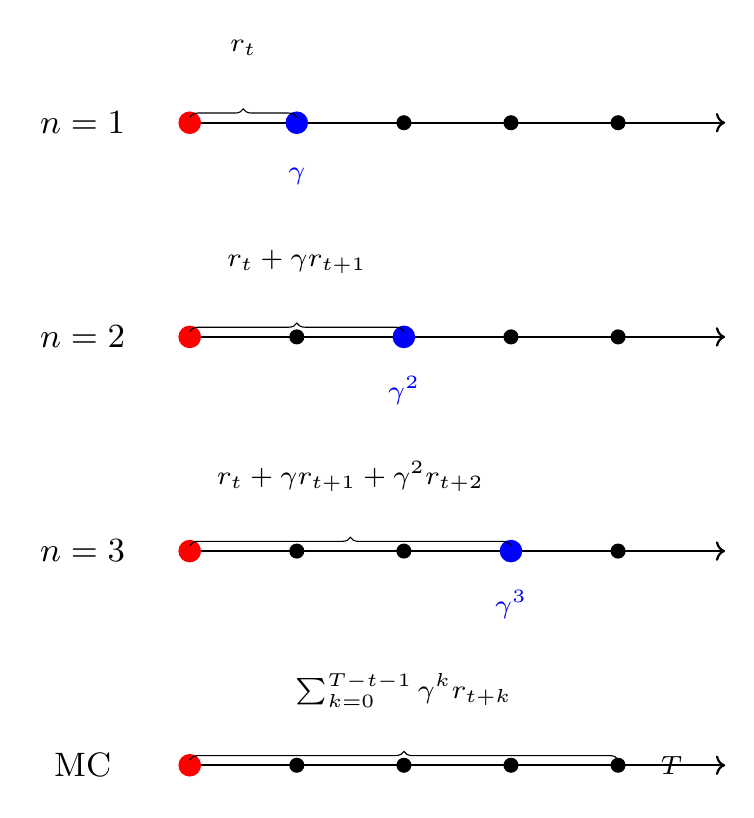
\begin{tikzpicture}[scale=0.85]
        % n=1
        \begin{scope}[shift={(0,0)}]
            \draw[->, thick] (0,0) -- (5,0);
            \foreach \x in {0,1,2,3,4} \fill (\x, 0) circle (2pt);
            \fill[red] (0,0) circle (3pt);
            \fill[blue] (1,0) circle (3pt);
            \draw[decorate, decoration={brace, amplitude=3pt, raise=2pt}] (0,0) -- (1,0);
            \node[font=\scriptsize] at (0.5, 0.7) {$r_t$};
            \node[font=\scriptsize, blue] at (1, -0.5) {$\gamma\Val$};
            \node[font=\small] at (-1, 0) {$n=1$};
        \end{scope}

        % n=2
        \begin{scope}[shift={(0,-2)}]
            \draw[->, thick] (0,0) -- (5,0);
            \foreach \x in {0,1,2,3,4} \fill (\x, 0) circle (2pt);
            \fill[red] (0,0) circle (3pt);
            \fill[blue] (2,0) circle (3pt);
            \draw[decorate, decoration={brace, amplitude=3pt, raise=2pt}] (0,0) -- (2,0);
            \node[font=\scriptsize] at (1, 0.7) {$r_t + \gamma r_{t+1}$};
            \node[font=\scriptsize, blue] at (2, -0.5) {$\gamma^2\Val$};
            \node[font=\small] at (-1, 0) {$n=2$};
        \end{scope}

        % n=3
        \begin{scope}[shift={(0,-4)}]
            \draw[->, thick] (0,0) -- (5,0);
            \foreach \x in {0,1,2,3,4} \fill (\x, 0) circle (2pt);
            \fill[red] (0,0) circle (3pt);
            \fill[blue] (3,0) circle (3pt);
            \draw[decorate, decoration={brace, amplitude=3pt, raise=2pt}] (0,0) -- (3,0);
            \node[font=\scriptsize] at (1.5, 0.7) {$r_t + \gamma r_{t+1} + \gamma^2 r_{t+2}$};
            \node[font=\scriptsize, blue] at (3, -0.5) {$\gamma^3\Val$};
            \node[font=\small] at (-1, 0) {$n=3$};
        \end{scope}

        % MC
        \begin{scope}[shift={(0,-6)}]
            \draw[->, thick] (0,0) -- (5,0);
            \foreach \x in {0,1,2,3,4} \fill (\x, 0) circle (2pt);
            \fill[red] (0,0) circle (3pt);
            \node[font=\scriptsize] at (4.5, 0) {$T$};
            \draw[decorate, decoration={brace, amplitude=3pt, raise=2pt}] (0,0) -- (4,0);
            \node[font=\scriptsize] at (2, 0.7) {$\sum_{k=0}^{T-t-1} \gamma^k r_{t+k}$};
            \node[font=\small] at (-1, 0) {MC};
        \end{scope}
    \end{tikzpicture}
    \caption{不同 $n$ 值下的 n-step return。红点为当前状态,蓝点为 Bootstrap 位置。}
    \label{fig:n-step-returns}
\end{figure}

\subsubsection{TD($\lambda$):加权平均}

TD($\lambda$) 方法将所有 n-step return 加权平均,而不是选择单一的 $n$:

\begin{definition}[$\lambda$-return]
\begin{equation}
    G_t^\lambda = (1-\lambda) \sum_{n=1}^{\infty} \lambda^{n-1} G_t^{(n)}
    \label{eq:lambda-return}
\end{equation}
其中 $\lambda \in [0,1]$ 控制权重的衰减速度。
\end{definition}

权重分布的直觉:
\begin{itemize}
    \item $G_t^{(1)}$ 的权重:$(1-\lambda)$
    \item $G_t^{(2)}$ 的权重:$(1-\lambda)\lambda$
    \item $G_t^{(n)}$ 的权重:$(1-\lambda)\lambda^{n-1}$
    \item 权重之和为 1
\end{itemize}

\begin{figure}[H]
    \centering
    \begin{tikzpicture}
        \begin{axis}[
            width=10cm, height=5cm,
            ybar,
            xlabel={$n$},
            ylabel={权重},
            symbolic x coords={1,2,3,4,5,$\cdots$,MC},
            xtick=data,
            ymin=0, ymax=0.6,
            bar width=12pt,
            nodes near coords,
            nodes near coords style={font=\tiny},
            every node near coord/.append style={yshift=3pt}
        ]
        % lambda = 0.5
        \addplot[fill=blue!60] coordinates {(1,0.5) (2,0.25) (3,0.125) (4,0.0625) (5,0.03125) ($\cdots$,0) (MC,0.03125)};
        \end{axis}
    \end{tikzpicture}
    \caption{$\lambda$-return 的权重分布($\lambda=0.5$)。短期 return 权重大,长期 return 权重指数衰减。}
    \label{fig:lambda-weights}
\end{figure}

特殊情况:
\begin{itemize}
    \item $\lambda = 0$:$G_t^\lambda = G_t^{(1)}$,等价于 TD(0)
    \item $\lambda = 1$:$G_t^\lambda = G_t^{(\infty)}$,等价于 Monte Carlo
\end{itemize}

\subsubsection{Eligibility Traces}

直接计算 $G_t^\lambda$ 需要等到 episode 结束。Eligibility Traces 提供了一种在线计算的方式。

\begin{definition}[Eligibility Trace]
为每个状态维护一个 eligibility trace $e_t(s)$:
\begin{equation}
    e_t(s) = \begin{cases}
        \gamma \lambda e_{t-1}(s) + 1 & \text{if } s = S_t \\
        \gamma \lambda e_{t-1}(s) & \text{otherwise}
    \end{cases}
\end{equation}
初始时 $e_0(s) = 0$ 对所有 $s$。
\end{definition}

TD($\lambda$) 的在线更新:
\begin{equation}
    \Val(s) \leftarrow \Val(s) + \alpha \delta_t e_t(s), \quad \forall s
\end{equation}
其中 $\delta_t = r_t + \gamma \Val(S_{t+1}) - \Val(S_t)$ 是 TD 误差。

\begin{keypoint}
Eligibility Trace 的直觉:
\begin{itemize}
    \item $e_t(s)$ 表示状态 $s$ 对当前 TD 误差的"责任"
    \item 刚访问过的状态责任大,随时间指数衰减
    \item 当 $\delta_t \neq 0$ 时,所有有责任的状态都被更新
\end{itemize}
这实现了"信用分配":奖励信号向过去的状态传播。
\end{keypoint}

% ------------------------------------------
\section{Q-Learning 与 SARSA}
\label{sec:q-learning-sarsa}

前面讨论的 MC 和 TD 方法是对 $\Val^\policy$ 的估计。为了找到最优策略,我们需要估计动作价值函数 $\Qval$,这样才能通过 $\argmax$ 导出策略。

\subsection{On-policy vs Off-policy}

\begin{definition}[On-policy 与 Off-policy]
\leavevmode
\begin{itemize}
    \item \textbf{On-policy}:评估和改进的是同一个策略
    \begin{itemize}
        \item 行为策略(收集数据)= 目标策略(被评估/改进)
        \item 例子:SARSA
    \end{itemize}
    \item \textbf{Off-policy}:用行为策略收集数据,评估/改进不同的目标策略
    \begin{itemize}
        \item 行为策略(收集数据)$\neq$ 目标策略(被评估/改进)
        \item 例子:Q-Learning
    \end{itemize}
\end{itemize}
\end{definition}

\begin{figure}[H]
    \centering
    \begin{tikzpicture}[
        box/.style={draw, rounded corners, minimum width=2cm, minimum height=1cm, align=center},
        arrow/.style={->, thick}
    ]
        % On-policy
        \begin{scope}[shift={(-4,0)}]
            \node[font=\bfseries] at (0, 2) {On-policy};
            \node[box, fill=blue!20] (behavior1) at (0, 0.5) {行为策略\\$\policy$};
            \node[box, fill=blue!20] (target1) at (0, -1.5) {目标策略\\$\policy$};
            \draw[arrow, <->] (behavior1) -- node[right, font=\scriptsize] {相同} (target1);
        \end{scope}

        % Off-policy
        \begin{scope}[shift={(4,0)}]
            \node[font=\bfseries] at (0, 2) {Off-policy};
            \node[box, fill=orange!20] (behavior2) at (-1.5, 0.5) {行为策略\\$\mu$};
            \node[box, fill=green!20] (target2) at (1.5, 0.5) {目标策略\\$\policy$};
            \node[box, fill=gray!20] (data) at (0, -1.5) {数据};
            \draw[arrow] (behavior2) -- (data);
            \draw[arrow] (data) -- (target2);
            \node[font=\scriptsize, red] at (0, 1) {不同};
        \end{scope}
    \end{tikzpicture}
    \caption{On-policy vs Off-policy。Off-policy 方法可以从任意行为策略的数据中学习目标策略。}
    \label{fig:on-off-policy}
\end{figure}

Off-policy 的优势:
\begin{itemize}
    \item 可以从历史数据(Experience Replay)中学习
    \item 可以从人类演示或其他策略的数据中学习
    \item 可以同时学习多个目标策略
\end{itemize}

\subsection{SARSA 算法}

SARSA 是一种 On-policy TD 控制方法,名字来自更新所需的五元组 $(S_t, A_t, R_t, S_{t+1}, A_{t+1})$。

\begin{definition}[SARSA 更新]
\begin{equation}
    \Qval(S_t, A_t) \leftarrow \Qval(S_t, A_t) + \alpha \left( r_t + \discount \Qval(S_{t+1}, A_{t+1}) - \Qval(S_t, A_t) \right)
    \label{eq:sarsa-update}
\end{equation}
其中 $A_{t+1}$ 是按当前策略(如 $\epsilon$-greedy)实际采样的动作。
\end{definition}

\begin{algorithm}[H]
\caption{SARSA}
\label{alg:sarsa}
\KwInput{学习率 $\alpha$,探索率 $\epsilon$,折扣因子 $\discount$}
初始化 $\Qval(s,a)$ 为任意值,$\Qval(\text{terminal}, \cdot) = 0$\;
\ForEach{episode}{
    初始化状态 $S$\;
    用 $\epsilon$-greedy 选择动作 $A$\;
    \Repeat{$S$ 是终止状态}{
        执行 $A$,观察 $R, S'$\;
        用 $\epsilon$-greedy 选择 $A'$\;
        $\Qval(S,A) \leftarrow \Qval(S,A) + \alpha \left( R + \discount \Qval(S',A') - \Qval(S,A) \right)$\;
        $S \leftarrow S'$, $A \leftarrow A'$\;
    }
}
\end{algorithm}

SARSA 学习的是当前策略(包括探索)的价值函数 $\Qval^\policy$,因此是 On-policy 的。

\subsection{Q-Learning 算法}

Q-Learning 是一种 Off-policy TD 控制方法,直接逼近最优 $\Qval^*$,而非当前策略的 $\Qval^\policy$。

\begin{definition}[Q-Learning 更新]
\begin{equation}
    \Qval(S_t, A_t) \leftarrow \Qval(S_t, A_t) + \alpha \left( r_t + \discount \max_{a'} \Qval(S_{t+1}, a') - \Qval(S_t, A_t) \right)
    \label{eq:q-learning-update}
\end{equation}
\end{definition}

关键区别:SARSA 使用 $\Qval(S_{t+1}, A_{t+1})$(实际采样的动作),Q-Learning 使用 $\max_{a'} \Qval(S_{t+1}, a')$(最优动作)。

\begin{theorem}[Q-Learning 收敛性]
\label{thm:q-learning-convergence}
在满足以下条件时,Q-Learning 收敛到 $\Qval^*$:
\begin{enumerate}
    \item 所有状态-动作对被无限次访问
    \item 学习率满足 Robbins-Monro 条件:$\sum_t \alpha_t = \infty$,$\sum_t \alpha_t^2 < \infty$
\end{enumerate}
\end{theorem}

\begin{proof}[证明思路]
Q-Learning 的更新可以写成随机近似(Stochastic Approximation)形式:
\begin{equation}
    \Qval_{t+1}(s,a) = (1 - \alpha_t) \Qval_t(s,a) + \alpha_t \left( r + \discount \max_{a'} \Qval_t(s', a') \right)
\end{equation}

这是对 Bellman Optimality 算子的随机逼近。由于 Bellman Optimality 算子是 $\gamma$-收缩的(定理 \ref{thm:bellman-contraction}),在 Robbins-Monro 条件下,随机近似收敛到不动点 $\Qval^*$。
\end{proof}

\begin{algorithm}[H]
\caption{Q-Learning}
\label{alg:q-learning}
\KwInput{学习率 $\alpha$,探索率 $\epsilon$,折扣因子 $\discount$}
初始化 $\Qval(s,a)$ 为任意值,$\Qval(\text{terminal}, \cdot) = 0$\;
\ForEach{episode}{
    初始化状态 $S$\;
    \Repeat{$S$ 是终止状态}{
        用 $\epsilon$-greedy 选择动作:$A = \begin{cases} \argmax_a \Qval(S,a) & \text{以概率 } 1-\epsilon \\ \text{随机动作} & \text{以概率 } \epsilon \end{cases}$\;
        执行 $A$,观察 $R, S'$\;
        $\Qval(S,A) \leftarrow \Qval(S,A) + \alpha \left( R + \discount \max_{a'} \Qval(S',a') - \Qval(S,A) \right)$\;
        $S \leftarrow S'$\;
    }
}
\end{algorithm}

\subsection{$\epsilon$-greedy 探索策略}

为了保证充分探索,常用 $\epsilon$-greedy 策略:

\begin{definition}[$\epsilon$-greedy]
\begin{equation}
    \policy(a|s) = \begin{cases}
        1 - \epsilon + \frac{\epsilon}{|\actionspace|} & \text{if } a = \argmax_{a'} \Qval(s,a') \\
        \frac{\epsilon}{|\actionspace|} & \text{otherwise}
    \end{cases}
\end{equation}
\end{definition}

\begin{itemize}
    \item $\epsilon = 0$:纯贪心(Greedy),无探索
    \item $\epsilon = 1$:纯随机,无利用
    \item 通常 $\epsilon$ 随训练逐渐衰减(如 $\epsilon_t = \epsilon_0 / t$)
\end{itemize}

\subsection{Cliff Walking 示例:Q-Learning vs SARSA}

Cliff Walking 是一个经典的 Grid World 环境,清晰展示了 Q-Learning 和 SARSA 的行为差异。

\begin{figure}[H]
    \centering
    \begin{tikzpicture}[scale=0.8]
        % Grid
        \foreach \x in {0,1,2,3,4,5,6,7,8,9,10,11} {
            \foreach \y in {0,1,2,3} {
                \draw (\x, \y) rectangle (\x+1, \y+1);
            }
        }

        % Cliff
        \foreach \x in {1,2,3,4,5,6,7,8,9,10} {
            \fill[red!30] (\x, 0) rectangle (\x+1, 1);
        }
        \node[font=\small] at (5.5, 0.5) {悬崖 ($r = -100$)};

        % Start and Goal
        \fill[green!30] (0, 0) rectangle (1, 1);
        \node[font=\small] at (0.5, 0.5) {S};
        \fill[blue!30] (11, 0) rectangle (12, 1);
        \node[font=\small] at (11.5, 0.5) {G};

        % Q-Learning path (optimal but risky)
        \draw[->, ultra thick, blue, dashed] (0.5, 0.5) -- (0.5, 0.8);
        \draw[->, ultra thick, blue] (0.5, 0.5) -- (11.5, 0.5);
        \node[font=\scriptsize, blue] at (6, -0.5) {Q-Learning 路径(最短但危险)};

        % SARSA path (safe)
        \draw[->, ultra thick, orange] (0.5, 0.7) -- (0.5, 1.5) -- (11.5, 1.5) -- (11.5, 0.7);
        \node[font=\scriptsize, orange] at (6, 2) {SARSA 路径(安全)};

        % Rewards
        \node[font=\tiny] at (-0.8, 2) {每步 $r=-1$};
    \end{tikzpicture}
    \caption{Cliff Walking 环境。S 是起点,G 是终点,红色区域是悬崖(掉下去 $r=-100$ 并回到 S)。Q-Learning 学习最优路径(沿悬崖边),SARSA 学习安全路径(远离悬崖)。}
    \label{fig:cliff-walking}
\end{figure}

\begin{keypoint}
Q-Learning vs SARSA 在 Cliff Walking 中的行为:
\begin{itemize}
    \item \textbf{Q-Learning}:学习最优路径(假设执行时不探索),即沿悬崖边走
    \begin{itemize}
        \item 但训练时因 $\epsilon$-greedy 探索,经常掉下悬崖
        \item 学到的 Q 值反映"如果完美执行"的价值
    \end{itemize}
    \item \textbf{SARSA}:学习考虑探索的保守路径,远离悬崖边缘
    \begin{itemize}
        \item 训练时更安全,掉崖次数少
        \item 学到的 Q 值反映"带探索执行"的价值
    \end{itemize}
\end{itemize}
根本原因:SARSA 的目标包含实际执行的探索动作 $A_{t+1}$,Q-Learning 的目标总是选 $\max$。
\end{keypoint}

\begin{table}[H]
    \centering
    \begin{tabular}{@{}lcc@{}}
        \toprule
        & \textbf{Q-Learning} & \textbf{SARSA} \\
        \midrule
        类型 & Off-policy & On-policy \\
        TD target & $r + \discount \max_{a'} \Qval(s',a')$ & $r + \discount \Qval(s', a')$ \\
        学习目标 & $\Qval^*$(最优策略) & $\Qval^\policy$(当前策略) \\
        行为 & 更激进/乐观 & 更保守 \\
        样本效率 & 高(可复用数据) & 低(只用当前策略数据) \\
        适合场景 & 安全代价低、需最优解 & 安全代价高、需稳定训练 \\
        \bottomrule
    \end{tabular}
    \caption{Q-Learning 与 SARSA 的全面对比}
    \label{tab:q-sarsa-comparison}
\end{table}

% ------------------------------------------
\section{Deep Q-Network (DQN)}
\label{sec:dqn}

表格 Q-Learning 无法处理大状态空间(如图像输入)或连续状态空间。DQN 使用神经网络逼近 $\Qval^*$,是深度强化学习的开创性工作。

\subsection{函数逼近的动机}

表格方法的局限:
\begin{itemize}
    \item \textbf{状态空间爆炸}:Atari 游戏的像素空间约 $256^{210 \times 160 \times 3} \approx 10^{90000}$
    \item \textbf{无法泛化}:没见过的状态无法处理
    \item \textbf{连续状态}:无法用表格表示机器人关节角度等连续变量
\end{itemize}

解决方案:用参数化函数 $\Qval(s,a;\theta)$(如神经网络)逼近 $\Qval^*$。

\begin{figure}[H]
    \centering
    \begin{tikzpicture}[
        layer/.style={draw, minimum width=1.5cm, minimum height=0.8cm, rounded corners},
        arrow/.style={->, thick}
    ]
        % Input
        \node[layer, fill=blue!20] (input) at (0, 0) {状态 $s$};
        \node[font=\scriptsize, below=0.1cm of input] {(图像/向量)};

        % Hidden layers
        \node[layer, fill=orange!20] (h1) at (3, 0) {隐藏层};
        \node[layer, fill=orange!20] (h2) at (5.5, 0) {隐藏层};

        % Output
        \node[layer, fill=green!20] (output) at (8.5, 0) {$\Qval(s, \cdot)$};
        \node[font=\scriptsize, below=0.1cm of output] {各动作的 Q 值};

        % Arrows
        \draw[arrow] (input) -- (h1);
        \draw[arrow] (h1) -- (h2);
        \draw[arrow] (h2) -- (output);

        % Q values
        \node[font=\scriptsize] at (10.5, 0.3) {$\Qval(s, a_1)$};
        \node[font=\scriptsize] at (10.5, 0) {$\Qval(s, a_2)$};
        \node[font=\scriptsize] at (10.5, -0.3) {$\vdots$};

        % Action selection
        \draw[arrow, red] (9.5, 0) -- (11, 0) node[right, font=\scriptsize] {$\argmax$};
    \end{tikzpicture}
    \caption{DQN 网络结构示意图。输入状态,输出各动作的 Q 值。选择 Q 值最大的动作。}
    \label{fig:dqn-architecture}
\end{figure}

\subsection{DQN 损失函数}

将 Q-Learning 更新转化为回归问题:

\begin{definition}[DQN 损失函数]
\begin{equation}
    \mathcal{L}(\theta) = \E_{(s,a,r,s') \sim \mathcal{D}} \left[ \left( \underbrace{r + \discount \max_{a'} \Qval(s',a';\theta^-)}_{\text{TD target } y} - \Qval(s,a;\theta) \right)^2 \right]
    \label{eq:dqn-loss}
\end{equation}
其中 $\mathcal{D}$ 是 Replay Buffer,$\theta^-$ 是 Target Network 的参数。
\end{definition}

梯度计算:
\begin{equation}
    \nabla_\theta \mathcal{L}(\theta) = \E \left[ -2(y - \Qval(s,a;\theta)) \nabla_\theta \Qval(s,a;\theta) \right]
\end{equation}

注意:$y$ 关于 $\theta$ 的梯度被忽略(因为用 $\theta^-$ 计算)。这是一种半梯度(semi-gradient)方法。

\subsection{Experience Replay}

\begin{definition}[Experience Replay]
将转移 $(s_t, a_t, r_t, s_{t+1})$ 存入 Replay Buffer $\mathcal{D}$,训练时从 $\mathcal{D}$ 中均匀随机采样 mini-batch。
\end{definition}

\begin{figure}[H]
    \centering
    \begin{tikzpicture}[scale=0.85]
        % Buffer
        \draw[thick] (0, 0) rectangle (8, 2);
        \node[font=\bfseries] at (4, 2.5) {Replay Buffer $\mathcal{D}$};

        % Transitions
        \draw[fill=blue!20] (0.2, 0.3) rectangle (0.8, 1.7);
        \node[font=\tiny] at (0.5, 1) {老};
        \draw[fill=blue!20] (1.7, 0.3) rectangle (2.3, 1.7);
        \node[font=\tiny] at (2, 1) {$\cdots$};
        \draw[fill=blue!20] (3.7, 0.3) rectangle (4.3, 1.7);
        \node[font=\tiny] at (4, 1) {$\cdots$};
        \draw[fill=blue!20] (5.7, 0.3) rectangle (6.3, 1.7);
        \node[font=\tiny] at (6, 1) {$\cdots$};
        \draw[fill=blue!20] (7.2, 0.3) rectangle (7.8, 1.7);
        \node[font=\tiny] at (7.5, 1) {新};

        % Write
        \draw[->, thick, red] (9, 1) -- (8.2, 1);
        \node[font=\scriptsize, red] at (10, 1) {写入新转移};

        % Sample
        \draw[->, thick, green!60!black] (2, -0.2) -- (2, -1);
        \draw[->, thick, green!60!black] (4, -0.2) -- (4, -1);
        \draw[->, thick, green!60!black] (6, -0.2) -- (6, -1);
        \node[font=\scriptsize, green!60!black] at (4, -1.5) {随机采样 mini-batch};

        % FIFO
        \draw[->, thick, gray] (-0.2, 1) -- (-1, 1);
        \node[font=\scriptsize, gray] at (-1.5, 1) {淘汰};
    \end{tikzpicture}
    \caption{Experience Replay 机制。新转移写入 Buffer,旧转移被淘汰(FIFO),训练时随机采样。}
    \label{fig:experience-replay}
\end{figure}

Experience Replay 的好处:
\begin{enumerate}
    \item \textbf{打破样本相关性}:连续收集的样本高度相关(同一轨迹),随机采样提供更独立的样本,符合 i.i.d. 假设
    \item \textbf{提高数据效率}:每个样本可被多次使用,而非用一次就丢弃
    \item \textbf{稳定数据分布}:Buffer 中的数据分布变化缓慢,训练更稳定
\end{enumerate}

\subsection{Target Network}

\begin{definition}[Target Network]
使用一组旧参数 $\theta^-$ 计算 TD target,定期更新 $\theta^- \leftarrow \theta$(如每 $C$ 步)。
\end{definition}

\begin{figure}[H]
    \centering
    \begin{tikzpicture}
        % Main network
        \node[draw, rounded corners, fill=blue!20, minimum width=3cm, minimum height=1.5cm] (main) at (0, 0) {主网络 $\Qval(\cdot; \theta)$};

        % Target network
        \node[draw, rounded corners, fill=orange!20, minimum width=3cm, minimum height=1.5cm] (target) at (6, 0) {目标网络 $\Qval(\cdot; \theta^-)$};

        % Update arrows
        \draw[->, thick] (main.north) -- ++(0, 1) -- ++(4.5, 0) -- (target.north);
        \node[font=\scriptsize] at (3, 1.3) {每 $C$ 步:$\theta^- \leftarrow \theta$};

        % Loss arrow - target network provides y for loss calculation
        \draw[->, thick, red] (target.west) -- (main.east) node[midway, above, font=\scriptsize] {提供 target $y$};

        % Gradient
        \draw[->, thick, green!60!black] (main.south) -- ++(0, -0.8) node[below, font=\scriptsize] {梯度更新 $\theta$};
    \end{tikzpicture}
    \caption{Target Network 机制。目标网络参数 $\theta^-$ 延迟更新,提供稳定的 TD target。}
    \label{fig:target-network}
\end{figure}

Target Network 的作用:
\begin{itemize}
    \item 避免目标"追着当前估计跑"导致的震荡或发散
    \item TD target 在一段时间内保持固定,类似于监督学习的固定标签
    \item 虽然引入了一定的偏差(使用旧参数),但显著提高了稳定性
\end{itemize}

\begin{note}
另一种变体是\textbf{软更新}(Soft Update):
\begin{equation}
    \theta^- \leftarrow \tau \theta + (1 - \tau) \theta^-
\end{equation}
其中 $\tau \ll 1$(如 $\tau = 0.005$)。这在 TD3、SAC 等算法中广泛使用。
\end{note}

\subsection{DQN 完整算法}

\begin{algorithm}[H]
\caption{Deep Q-Network (DQN)}
\label{alg:dqn}
\KwInput{Replay Buffer 容量 $N$,Mini-batch 大小 $B$,Target 更新频率 $C$,探索衰减参数}
初始化 Replay Buffer $\mathcal{D}$,容量 $N$\;
初始化 Q 网络参数 $\theta$(随机)\;
初始化 Target 网络参数 $\theta^- \leftarrow \theta$\;
\ForEach{episode}{
    初始化状态 $s_1$(预处理,如堆叠 4 帧)\;
    \For{$t = 1, 2, \ldots, T$}{
        以概率 $\epsilon$ 随机选择动作 $a_t$,否则 $a_t = \argmax_a \Qval(s_t, a; \theta)$\;
        执行 $a_t$,观察 $r_t, s_{t+1}$\;
        存储转移 $(s_t, a_t, r_t, s_{t+1})$ 到 $\mathcal{D}$\;
        从 $\mathcal{D}$ 随机采样 mini-batch:$\{(s_j, a_j, r_j, s'_j)\}_{j=1}^B$\;
        计算 TD target:$y_j = \begin{cases} r_j & \text{if } s'_j \text{ 是终止状态} \\ r_j + \gamma \max_{a'} \Qval(s'_j, a'; \theta^-) & \text{otherwise} \end{cases}$\;
        梯度下降:$\theta \leftarrow \theta - \alpha \nabla_\theta \frac{1}{B} \sum_j (y_j - \Qval(s_j, a_j; \theta))^2$\;
        每 $C$ 步:$\theta^- \leftarrow \theta$\;
        衰减 $\epsilon$\;
    }
}
\end{algorithm}

\begin{important}
DQN 的两个关键技巧解决了深度 RL 的稳定性问题:
\begin{enumerate}
    \item \textbf{Experience Replay}:解决样本相关性问题,提高数据效率
    \item \textbf{Target Network}:解决目标不稳定问题,避免震荡发散
\end{enumerate}
这两个技巧至今仍是 Value-Based 深度 RL 的标准做法。
\end{important}

\subsection{DQN 变体}

原始 DQN 存在一些问题,后续工作提出了多种改进。

\subsubsection{Double DQN}

原始 DQN 使用同一个网络选择动作和评估价值,导致\textbf{过估计}(Overestimation)问题。

\begin{definition}[过估计问题]
$\max$ 操作天然倾向于选择被高估的动作:
\begin{equation}
    \E\left[ \max_a \Qval(s, a) \right] \geq \max_a \E[\Qval(s, a)]
\end{equation}
当 $\Qval$ 有估计噪声时,$\max$ 会放大正向误差。
\end{definition}

\begin{definition}[Double DQN]
解耦动作选择和价值评估:
\begin{equation}
    y = r + \discount \Qval\left(s', \argmax_{a'} \Qval(s',a';\theta); \theta^-\right)
\end{equation}
\begin{itemize}
    \item 用\textbf{当前网络} $\theta$ 选择动作:$a^* = \argmax_{a'} \Qval(s',a';\theta)$
    \item 用\textbf{Target 网络} $\theta^-$ 评估价值:$\Qval(s', a^*; \theta^-)$
\end{itemize}
\end{definition}

\subsubsection{Dueling DQN}

将 Q 值分解为状态价值和动作优势:

\begin{definition}[Dueling DQN]
\begin{equation}
    \Qval(s,a;\theta) = \Val(s;\theta_v) + \left( \advantage(s,a;\theta_a) - \frac{1}{|\actionspace|} \sum_{a'} \advantage(s,a';\theta_a) \right)
\end{equation}
其中 $\Val$ 和 $\advantage$ 共享前几层特征,最后分叉。减去均值是为了可辨识性(identifiability)。
\end{definition}

\begin{figure}[H]
    \centering
    \begin{tikzpicture}[scale=0.8]
        % Shared layers
        \node[draw, rounded corners, fill=blue!20, minimum width=2cm, minimum height=1cm] (shared) at (0, 0) {共享层};

        % Value stream
        \node[draw, rounded corners, fill=green!20, minimum width=1.5cm, minimum height=0.8cm] (v) at (-2, -2) {$\Val(s)$};

        % Advantage stream
        \node[draw, rounded corners, fill=orange!20, minimum width=1.5cm, minimum height=0.8cm] (a) at (2, -2) {$\advantage(s,a)$};

        % Combine
        \node[draw, rounded corners, fill=purple!20, minimum width=2cm, minimum height=0.8cm] (q) at (0, -4) {$\Qval(s,a)$};

        % Arrows
        \draw[->, thick] (shared) -- (v);
        \draw[->, thick] (shared) -- (a);
        \draw[->, thick] (v) -- node[left, font=\scriptsize] {$+$} (q);
        \draw[->, thick] (a) -- node[right, font=\scriptsize] {$-\text{mean}$} (q);
    \end{tikzpicture}
    \caption{Dueling DQN 架构。分别估计 $\Val(s)$ 和 $\advantage(s,a)$,再组合成 $\Qval(s,a)$。}
    \label{fig:dueling-dqn}
\end{figure}

Dueling DQN 的优势:
\begin{itemize}
    \item 在某些状态下,所有动作的价值相近(如远离障碍物),分解结构允许网络直接学习状态价值
    \item 更高效地学习哪些状态是"好的",独立于具体动作
\end{itemize}

\subsubsection{其他改进}

\begin{itemize}
    \item \textbf{Prioritized Experience Replay}:优先采样 TD 误差大的样本
    \item \textbf{Multi-step Learning}:使用 n-step return 作为 target
    \item \textbf{Distributional RL}:学习回报的分布而非期望
    \item \textbf{Noisy Networks}:用网络参数噪声替代 $\epsilon$-greedy 探索
\end{itemize}

Rainbow 将上述所有改进组合,在 Atari 游戏上取得了 SOTA 性能。

% ------------------------------------------
\section{本章小结}
\label{sec:value-summary}

\begin{keypoint}
本章核心内容:
\begin{enumerate}
    \item \textbf{Bellman 方程}是 Value-Based RL 的理论基础
    \begin{itemize}
        \item Bellman Expectation:描述给定策略的价值
        \item Bellman Optimality:描述最优策略的价值
        \item Bellman 算子是 $\gamma$-收缩映射,保证迭代收敛
    \end{itemize}

    \item \textbf{动态规划}(模型已知时)
    \begin{itemize}
        \item Policy Evaluation:迭代求解 $\Val^\policy$
        \item Policy Iteration:评估 $\to$ 改进 $\to$ 评估 $\to$ $\cdots$
        \item Value Iteration:直接迭代 Bellman Optimality 方程
    \end{itemize}

    \item \textbf{MC vs TD}(模型未知时)
    \begin{itemize}
        \item MC:无偏高方差,需完整轨迹
        \item TD:有偏低方差,每步更新
        \item n-step TD 和 TD($\lambda$) 在两者之间权衡
    \end{itemize}

    \item \textbf{Q-Learning vs SARSA}
    \begin{itemize}
        \item Q-Learning:Off-policy,学习 $\Qval^*$,更激进
        \item SARSA:On-policy,学习 $\Qval^\policy$,更保守
    \end{itemize}

    \item \textbf{DQN}:深度 Value-Based RL
    \begin{itemize}
        \item Experience Replay:打破样本相关性
        \item Target Network:稳定 TD target
        \item Double DQN、Dueling DQN 等改进
    \end{itemize}
\end{enumerate}
\end{keypoint}

\begin{note}
Value-Based 方法的局限性:
\begin{itemize}
    \item 只能处理离散动作空间($\argmax$ 需要枚举)
    \item 策略是隐式的,无法直接表示随机策略
    \item 对于高维动作空间,$\max$ 操作计算量大
\end{itemize}
这些局限促使了 Policy-Based 方法的发展,我们将在下一章详细介绍。
\end{note}


% 第三章:基于策略的强化学习
% ==========================================
% 第三章:基于策略的强化学习
% ==========================================

\chapter{基于策略的强化学习}
\label{chap:policy-based}

% ------------------------------------------
\section{引言:直接优化策略}
\label{sec:policy-intro}

\subsection{核心问题}

在第二章中,我们介绍了 Value-Based 方法:先学习 $\Qval^*$,再通过 $\argmax$ 导出策略。这种方法在离散动作空间中效果很好,但遇到以下问题时会遇到困难:

\begin{quote}
\textbf{如果动作空间是连续的(如机器人关节角度),如何计算 $\argmax_a \Qval(s,a)$?}

\textbf{如果最优策略是随机的(如石头剪刀布),如何用确定性策略表示?}
\end{quote}

Policy-Based 方法提供了一种更直接的思路:\textbf{直接参数化策略 $\policy_\theta(a|s)$,通过梯度上升最大化期望回报}。

\subsection{Value-Based 方法的局限性}

尽管 Q-Learning 和 DQN 取得了很大成功,但存在以下局限:

\begin{enumerate}
    \item \textbf{连续动作空间困难}:$\max_a \Qval(s,a)$ 需要枚举或优化所有动作,在连续空间中无法直接计算

    \item \textbf{函数逼近不稳定}(Deadly Triad):当同时使用函数逼近、Bootstrapping 和 Off-policy 学习时,算法可能发散

    \item \textbf{优化目标间接}:Value-Based 方法最小化 TD 误差,而非直接优化期望回报 $J(\policy)$

    \item \textbf{只能学习确定性策略}:$\argmax$ 输出确定动作,但在某些环境中随机策略更优(如博弈、部分可观测环境)
\end{enumerate}

\begin{figure}[H]
    \centering
    \begin{tikzpicture}[
        box/.style={draw, rounded corners, fill=blue!10, minimum width=3cm, minimum height=1.2cm, align=center},
        arrow/.style={->, thick, >=stealth}
    ]
        % Value-Based
        \begin{scope}[shift={(-4,0)}]
            \node[box, fill=orange!20] (q) at (0,0) {学习 $\Qval^*$};
            \node[box, fill=green!20] (pi) at (0,-2.5) {$\policy^* = \argmax$};
            \draw[arrow] (q) -- (pi);
            \node[font=\bfseries] at (0, 1.2) {Value-Based};
            \node[font=\scriptsize, red] at (0, -3.8) {需要枚举动作};
        \end{scope}

        % Policy-Based
        \begin{scope}[shift={(4,0)}]
            \node[box, fill=purple!20] (policy) at (0,-1.25) {直接学习 $\policy_\theta$};
            \node[font=\bfseries] at (0, 1.2) {Policy-Based};
            \node[font=\scriptsize, green!60!black] at (0, -3.8) {直接输出动作分布};
        \end{scope}

        % VS
        \node[font=\Large] at (0, -1.25) {vs};
    \end{tikzpicture}
    \caption{Value-Based vs. Policy-Based。前者间接导出策略,后者直接参数化策略。}
    \label{fig:value-vs-policy}
\end{figure}

\subsection{参数化策略}

Policy-Based 方法直接参数化策略 $\policy_\theta(a|s)$,通过梯度上升最大化期望回报:
\begin{equation}
    J(\theta) = \E_{\trajectory \sim \policy_\theta} \left[ G_0 \right] = \E_{\trajectory \sim \policy_\theta} \left[ \sum_{t=0}^{T} \discount^t r_t \right]
\end{equation}

策略参数化的常见形式:

\begin{itemize}
    \item \textbf{离散动作空间}:Softmax 输出 Categorical 分布
    \begin{equation}
        \policy_\theta(a|s) = \frac{\exp(f_\theta(s,a))}{\sum_{a'} \exp(f_\theta(s,a'))}
    \end{equation}

    \item \textbf{连续动作空间}:输出高斯分布的参数 $(\mu_\theta(s), \sigma_\theta(s))$
    \begin{equation}
        \policy_\theta(a|s) = \mathcal{N}(a \mid \mu_\theta(s), \sigma_\theta^2(s))
    \end{equation}
\end{itemize}

\begin{figure}[H]
    \centering
    \begin{tikzpicture}[scale=0.9]
        % Discrete
        \begin{scope}[shift={(-4,0)}]
            \node[font=\bfseries] at (0, 2) {离散动作};
            \draw[->] (-1.5, 0) -- (1.5, 0) node[right, font=\scriptsize] {动作};
            \draw[->] (-1.5, 0) -- (-1.5, 1.5) node[above, font=\scriptsize] {概率};

            % Bars
            \fill[blue!60] (-1, 0) rectangle (-0.5, 1.2);
            \fill[blue!60] (-0.2, 0) rectangle (0.3, 0.6);
            \fill[blue!60] (0.6, 0) rectangle (1.1, 0.3);

            \node[font=\tiny] at (-0.75, -0.3) {$a_1$};
            \node[font=\tiny] at (0.05, -0.3) {$a_2$};
            \node[font=\tiny] at (0.85, -0.3) {$a_3$};

            \node[font=\scriptsize] at (0, -1) {Softmax 输出};
        \end{scope}

        % Continuous
        \begin{scope}[shift={(4,0)}]
            \node[font=\bfseries] at (0, 2) {连续动作};
            \draw[->] (-2, 0) -- (2, 0) node[right, font=\scriptsize] {动作 $a$};
            \draw[->] (-2, 0) -- (-2, 1.5) node[above, font=\scriptsize] {概率密度};

            % Gaussian curve
            \draw[thick, blue, domain=-1.8:1.8, samples=50] plot (\x, {1.2*exp(-\x*\x/0.5)});

            \draw[dashed] (0, 0) -- (0, 1.2);
            \node[font=\tiny] at (0, -0.3) {$\mu_\theta(s)$};
            \draw[<->] (-0.7, 0.7) -- (0.7, 0.7);
            \node[font=\tiny] at (0, 0.9) {$\sigma_\theta(s)$};

            \node[font=\scriptsize] at (0, -1) {高斯分布输出};
        \end{scope}
    \end{tikzpicture}
    \caption{策略参数化:离散动作用 Softmax,连续动作用高斯分布}
    \label{fig:policy-parameterization}
\end{figure}

\begin{keypoint}
Policy-Based 方法的优势:
\begin{enumerate}
    \item \textbf{处理连续动作}:直接输出动作分布,无需 $\argmax$
    \item \textbf{学习随机策略}:可以输出动作的概率分布
    \item \textbf{直接优化目标}:梯度上升直接最大化 $J(\theta)$
    \item \textbf{更好的收敛性质}:策略参数的小变化导致策略的小变化(光滑)
\end{enumerate}
\end{keypoint}

% ------------------------------------------
\section{Policy Gradient 定理}
\label{sec:policy-gradient}

Policy Gradient 定理是 Policy-Based RL 的理论基础,它给出了目标函数 $J(\theta)$ 关于参数 $\theta$ 的梯度表达式。

\subsection{目标函数定义}

\begin{definition}[策略性能指标]
\begin{equation}
    J(\theta) = \E_{\trajectory \sim \policy_\theta} \left[ R(\trajectory) \right] = \int p(\trajectory | \theta) R(\trajectory) d\trajectory
\end{equation}
其中 $R(\trajectory) = G_0 = \sum_{t=0}^{T} \discount^t r_t$ 是轨迹的总回报。
\end{definition}

问题:如何计算 $\nabla_\theta J(\theta)$?

直接求导会遇到困难:$R(\trajectory)$ 依赖于环境动力学 $P(s'|s,a)$,而我们通常不知道 $P$。

\subsection{Log-Derivative Trick}

计算 $\nabla_\theta J(\theta)$ 的关键技巧是 \textbf{Log-Derivative Trick}(也称为 REINFORCE trick 或 Score Function):

\begin{lemma}[Log-Derivative Trick]
\label{lem:log-derivative}
对于任意概率分布 $p(x|\theta)$:
\begin{equation}
    \nabla_\theta p(x|\theta) = p(x|\theta) \nabla_\theta \log p(x|\theta)
\end{equation}
\end{lemma}

\begin{proof}
由对数的求导法则(链式法则):
\begin{equation}
    \nabla_\theta \log p(x|\theta) = \frac{\nabla_\theta p(x|\theta)}{p(x|\theta)}
\end{equation}
两边同乘 $p(x|\theta)$:
\begin{equation}
    p(x|\theta) \nabla_\theta \log p(x|\theta) = \nabla_\theta p(x|\theta)
\end{equation}
\end{proof}

\begin{note}
Log-Derivative Trick 的妙处:将对 $p(x|\theta)$ 的求导转化为对 $\log p(x|\theta)$ 的求导,而后者往往更容易计算,特别是当 $p$ 是乘积形式时。
\end{note}

\subsection{Policy Gradient 定理的完整推导}

\begin{theorem}[Policy Gradient Theorem]
\label{thm:policy-gradient}
\begin{equation}
    \nabla_\theta J(\theta) = \E_{\trajectory \sim \policy_\theta} \left[ \sum_{t=0}^{T} \nabla_\theta \log \policy_\theta(a_t|s_t) \cdot G_t \right]
    \label{eq:policy-gradient}
\end{equation}
其中 $G_t = \sum_{k=0}^{T-t} \discount^k r_{t+k}$ 是从时刻 $t$ 开始的 reward-to-go。
\end{theorem}

\begin{proof}
\textbf{Step 1}:应用 Log-Derivative Trick

从目标函数的定义出发:
\begin{align}
    \nabla_\theta J(\theta) &= \nabla_\theta \int p(\trajectory|\theta) R(\trajectory) d\trajectory \\
    &= \int \nabla_\theta p(\trajectory|\theta) R(\trajectory) d\trajectory \quad \text{(交换积分和求导)}\\
    &= \int p(\trajectory|\theta) \nabla_\theta \log p(\trajectory|\theta) R(\trajectory) d\trajectory \quad \text{(Log-Derivative Trick)}\\
    &= \E_{\trajectory \sim \policy_\theta} \left[ \nabla_\theta \log p(\trajectory|\theta) \cdot R(\trajectory) \right]
\end{align}

\textbf{Step 2}:展开 $\nabla_\theta \log p(\trajectory|\theta)$

回顾轨迹概率分解(第一章公式 \eqref{eq:trajectory-prob}):
\begin{equation}
    p(\trajectory|\theta) = p(s_0) \prod_{t=0}^{T-1} \policy_\theta(a_t|s_t) P(s_{t+1}|s_t,a_t)
\end{equation}

取对数:
\begin{equation}
    \log p(\trajectory|\theta) = \log p(s_0) + \sum_{t=0}^{T-1} \log \policy_\theta(a_t|s_t) + \sum_{t=0}^{T-1} \log P(s_{t+1}|s_t,a_t)
\end{equation}

对 $\theta$ 求梯度:
\begin{equation}
    \nabla_\theta \log p(\trajectory|\theta) = \underbrace{\nabla_\theta \log p(s_0)}_{=0} + \sum_{t=0}^{T-1} \nabla_\theta \log \policy_\theta(a_t|s_t) + \underbrace{\sum_{t=0}^{T-1} \nabla_\theta \log P(s_{t+1}|s_t,a_t)}_{=0}
\end{equation}

\begin{important}
\textbf{关键观察}:$p(s_0)$ 是环境的初始状态分布,$P(s_{t+1}|s_t,a_t)$ 是环境的动力学模型,它们都与策略参数 $\theta$ 无关,因此梯度为零!

最终:
\begin{equation}
    \nabla_\theta \log p(\trajectory|\theta) = \sum_{t=0}^{T-1} \nabla_\theta \log \policy_\theta(a_t|s_t)
    \label{eq:grad-log-trajectory}
\end{equation}

这意味着:\textbf{即使不知道环境动力学 $P$,我们也能计算 Policy Gradient}——这是 Policy Gradient 方法能够 Model-Free 的根本原因。
\end{important}

\textbf{Step 3}:代入得到基本形式

将 \eqref{eq:grad-log-trajectory} 代入:
\begin{equation}
    \nabla_\theta J(\theta) = \E_{\trajectory \sim \policy_\theta} \left[ \left( \sum_{t=0}^{T} \nabla_\theta \log \policy_\theta(a_t|s_t) \right) \cdot R(\trajectory) \right]
    \label{eq:pg-basic}
\end{equation}

\textbf{Step 4}:引入 Reward-to-go(因果性)

展开 \eqref{eq:pg-basic}:
\begin{equation}
    \nabla_\theta J(\theta) = \E \left[ \sum_{t=0}^{T} \nabla_\theta \log \policy_\theta(a_t|s_t) \cdot \sum_{t'=0}^{T} r_{t'} \right]
\end{equation}

考虑交叉项 $\nabla_\theta \log \policy_\theta(a_t|s_t) \cdot r_{t'}$,当 $t' < t$ 时:
\begin{itemize}
    \item $r_{t'}$ 是在时刻 $t'$ 获得的奖励,发生在动作 $a_t$ 之前
    \item $a_t$ 的选择不可能影响过去的奖励 $r_{t'}$
    \item 因此 $\E[\nabla_\theta \log \policy_\theta(a_t|s_t) \cdot r_{t'}] = 0$(由引理 \ref{lem:score-zero})
\end{itemize}

只有 $t' \geq t$ 的奖励才与 $a_t$ 相关,因此可以用 reward-to-go $G_t = \sum_{k=0}^{T-t} \discount^k r_{t+k}$ 替代 $R(\trajectory)$:
\begin{equation}
    \nabla_\theta J(\theta) = \E_{\trajectory \sim \policy_\theta} \left[ \sum_{t=0}^{T} \nabla_\theta \log \policy_\theta(a_t|s_t) \cdot G_t \right]
\end{equation}
\end{proof}

\begin{lemma}[Score Function 的期望为零]
\label{lem:score-zero}
对于任意策略 $\policy_\theta$:
\begin{equation}
    \E_{a \sim \policy_\theta(\cdot|s)} \left[ \nabla_\theta \log \policy_\theta(a|s) \right] = 0
\end{equation}
\end{lemma}

\begin{proof}
\begin{align}
    \E_{a \sim \policy_\theta} \left[ \nabla_\theta \log \policy_\theta(a|s) \right]
    &= \sum_a \policy_\theta(a|s) \cdot \frac{\nabla_\theta \policy_\theta(a|s)}{\policy_\theta(a|s)} \\
    &= \sum_a \nabla_\theta \policy_\theta(a|s) \\
    &= \nabla_\theta \sum_a \policy_\theta(a|s) \\
    &= \nabla_\theta 1 = 0
\end{align}
\end{proof}

\begin{figure}[H]
    \centering
    \begin{tikzpicture}[scale=0.85]
        % Timeline
        \draw[->, thick] (0,0) -- (12,0) node[right] {时间};

        % Time points
        \foreach \x/\t in {1/0, 3/1, 5/2, 7/t, 9/{t+1}, 11/T} {
            \fill (\x, 0) circle (2pt);
            \node[below] at (\x, -0.2) {$\t$};
        }

        % Actions
        \foreach \x in {1, 3, 5, 7, 9} {
            \node[above, font=\scriptsize, blue] at (\x, 0.3) {$a$};
        }

        % Rewards
        \foreach \x in {2, 4, 6, 8, 10} {
            \node[above, font=\scriptsize, red] at (\x, 0.6) {$r$};
        }

        % Highlight current action
        \fill[blue!30] (6.7, -0.3) rectangle (7.3, 0.3);
        \node[below, font=\small] at (7, -0.6) {当前动作 $a_t$};

        % Past rewards (not affected)
        \draw[decorate, decoration={brace, amplitude=5pt, raise=5pt, mirror}] (1,-0.8) -- (6,-0.8)
            node[midway, below=10pt, font=\scriptsize] {过去奖励:与 $a_t$ 无关};

        % Future rewards (affected)
        \draw[decorate, decoration={brace, amplitude=5pt, raise=5pt}] (7,0.9) -- (11,0.9)
            node[midway, above=8pt, font=\scriptsize] {$G_t = r_t + \gamma r_{t+1} + \cdots$};
    \end{tikzpicture}
    \caption{因果性:动作 $a_t$ 只影响未来奖励,不影响过去。因此 Policy Gradient 只需要 reward-to-go $G_t$。}
    \label{fig:causality}
\end{figure}

\begin{keypoint}
Policy Gradient 定理的直观理解:
\begin{itemize}
    \item $\nabla_\theta \log \policy_\theta(a_t|s_t)$ 是"增加动作 $a_t$ 概率"的方向
    \item $G_t$ 是该动作之后获得的累积奖励
    \item 如果 $G_t > 0$:沿梯度方向更新,增加 $a_t$ 的概率
    \item 如果 $G_t < 0$:反向更新,减少 $a_t$ 的概率
\end{itemize}
简言之:\textbf{好的动作更可能被选择,坏的动作更少被选择}。
\end{keypoint}

% ------------------------------------------
\section{REINFORCE 算法}
\label{sec:reinforce}

REINFORCE 是最简单的 Policy Gradient 算法,直接使用蒙特卡洛采样来估计梯度。

\begin{algorithm}[H]
\caption{REINFORCE}
\label{alg:reinforce}
\KwInput{学习率 $\alpha$,初始策略参数 $\theta$}
\ForEach{episode}{
    采样轨迹 $\trajectory = (s_0, a_0, r_0, \ldots, s_T)$ 按策略 $\policy_\theta$\;
    \ForEach{$t = 0, 1, \ldots, T$}{
        计算 $G_t = \sum_{k=0}^{T-t} \discount^k r_{t+k}$\;
    }
    更新参数:$\theta \leftarrow \theta + \alpha \sum_{t=0}^{T} \nabla_\theta \log \policy_\theta(a_t|s_t) \cdot G_t$\;
}
\end{algorithm}

\subsection{无偏性}

\begin{theorem}[REINFORCE 是无偏估计]
REINFORCE 的梯度估计:
\begin{equation}
    \hat{g} = \sum_{t=0}^{T} \nabla_\theta \log \policy_\theta(a_t|s_t) \cdot G_t
\end{equation}
是 $\nabla_\theta J(\theta)$ 的无偏估计,即 $\E[\hat{g}] = \nabla_\theta J(\theta)$。
\end{theorem}

\begin{proof}
这是 Policy Gradient 定理(定理 \ref{thm:policy-gradient})的直接推论。轨迹 $\tau$ 按 $\policy_\theta$ 采样,$G_t$ 是真实回报,期望就是 $\nabla_\theta J(\theta)$。
\end{proof}

\subsection{高方差问题}

尽管 REINFORCE 无偏,但方差很大:

\begin{itemize}
    \item $G_t$ 累积了从 $t$ 到终止的所有随机性(环境随机 + 策略随机)
    \item 轨迹越长,方差越大
    \item 奖励稀疏时,大部分轨迹的 $G_t \approx 0$,偶尔出现大的 $G_t$
    \item $G_t$ 包含了很多与具体动作 $a_t$ 无关的噪声
\end{itemize}

\begin{figure}[H]
    \centering
    \begin{tikzpicture}[scale=0.8]
        % Axis
        \draw[->] (0,0) -- (8,0) node[right] {Episode};
        \draw[->] (0,-2) -- (0,3) node[above] {$\hat{g}$(梯度估计)};

        % High variance samples
        \foreach \x in {1,2,3,4,5,6,7} {
            \pgfmathsetmacro{\y}{2*rand}
            \fill[blue] (\x, \y) circle (2pt);
        }

        % True gradient
        \draw[red, thick, dashed] (0, 0.5) -- (8, 0.5);
        \node[red, right] at (8, 0.5) {$\nabla J$};

        % Label
        \node[font=\scriptsize] at (4, -2.5) {高方差:每次估计波动很大};
    \end{tikzpicture}
    \caption{REINFORCE 的高方差问题示意图。虽然期望正确,但单次估计波动大。}
    \label{fig:reinforce-variance}
\end{figure}

% ------------------------------------------
\section{Baseline 与方差降低}
\label{sec:baseline}

\subsection{Baseline 技巧}

一个巧妙的技巧是:从 $G_t$ 中减去一个 baseline $b(s_t)$,可以降低方差而不引入偏差。

\begin{theorem}[Baseline 不改变期望]
\label{thm:baseline}
对于任意只依赖于状态 $s$(不依赖于动作 $a$)的函数 $b(s)$:
\begin{equation}
    \E_{a \sim \policy_\theta(\cdot|s)} \left[ \nabla_\theta \log \policy_\theta(a|s) \cdot b(s) \right] = 0
\end{equation}
\end{theorem}

\begin{proof}
由于 $b(s)$ 不依赖于 $a$,可以提出期望外:
\begin{align}
    \E_{a \sim \policy_\theta} \left[ \nabla_\theta \log \policy_\theta(a|s) \cdot b(s) \right]
    &= b(s) \cdot \E_{a \sim \policy_\theta} \left[ \nabla_\theta \log \policy_\theta(a|s) \right] \\
    &= b(s) \cdot \sum_a \policy_\theta(a|s) \cdot \frac{\nabla_\theta \policy_\theta(a|s)}{\policy_\theta(a|s)} \\
    &= b(s) \cdot \sum_a \nabla_\theta \policy_\theta(a|s) \\
    &= b(s) \cdot \nabla_\theta \underbrace{\sum_a \policy_\theta(a|s)}_{= 1} \\
    &= b(s) \cdot \nabla_\theta 1 = 0
\end{align}
\end{proof}

因此,Policy Gradient 可以写成:
\begin{equation}
    \nabla_\theta J(\theta) = \E \left[ \sum_t \nabla_\theta \log \policy_\theta(a_t|s_t) \cdot (G_t - b(s_t)) \right]
    \label{eq:pg-with-baseline}
\end{equation}

减去 baseline 不改变期望,但可以显著降低方差!

\subsection{为什么 Baseline 能降低方差?}

直觉解释:
\begin{itemize}
    \item $G_t$ 可能总是正的(如奖励都是正数),导致所有动作概率都被增加
    \item 减去 $b(s)$(如平均回报),使得 $G_t - b(s_t)$ 有正有负
    \item 好于平均的动作被增强,差于平均的动作被削弱
\end{itemize}

\begin{figure}[H]
    \centering
    \begin{tikzpicture}[scale=0.9]
        % Without baseline
        \begin{scope}[shift={(-4,0)}]
            \node[font=\bfseries] at (0, 3) {无 Baseline};
            \draw[->] (-1.5, 0) -- (1.5, 0) node[right, font=\scriptsize] {动作};
            \draw[->] (-1.5, 0) -- (-1.5, 2.3);
            \node[font=\scriptsize, anchor=south] at (-1.5, 2.3) {$G_t$};

            % All positive
            \fill[blue!60] (-1, 0) rectangle (-0.5, 1.8);
            \fill[blue!60] (-0.2, 0) rectangle (0.3, 1.2);
            \fill[blue!60] (0.6, 0) rectangle (1.1, 1.5);

            \node[font=\tiny, red] at (0, -0.5) {全正,所有动作都被增强};
        \end{scope}

        % With baseline
        \begin{scope}[shift={(4,0)}]
            \node[font=\bfseries] at (0, 3) {有 Baseline};
            \draw[->] (-1.5, 0) -- (1.5, 0) node[right, font=\scriptsize] {动作};
            \draw[->] (-1.5, -1) -- (-1.5, 2.3);
            \node[font=\scriptsize, anchor=south] at (-1.5, 2.3) {$G_t - b$};

            % Mixed
            \fill[green!60] (-1, 0) rectangle (-0.5, 1.0);
            \fill[red!60] (-0.2, 0) rectangle (0.3, -0.6);
            \fill[green!60] (0.6, 0) rectangle (1.1, 0.5);

            % Baseline
            \draw[dashed, gray] (-1.5, 0) -- (1.5, 0);
            \node[font=\tiny, gray, right] at (1.5, 0) {$b(s)$};

            \node[font=\tiny, green!60!black] at (0, -1.5) {好动作增强,坏动作削弱};
        \end{scope}
    \end{tikzpicture}
    \caption{Baseline 的效果:将"绝对好坏"变为"相对好坏",提供更清晰的学习信号。}
    \label{fig:baseline-effect}
\end{figure}

\subsection{最优 Baseline}

\begin{theorem}[最优 Baseline]
在不改变期望的前提下,使方差最小的 baseline 是状态价值函数:
\begin{equation}
    b^*(s) = \Val^\policy(s)
\end{equation}
\end{theorem}

\begin{proof}[证明思路]
方差 $\text{Var}[\hat{g}]$ 关于 $b(s)$ 是二次函数,对 $b(s)$ 求导并令其为零:
\begin{equation}
    \frac{\partial \text{Var}[\hat{g}]}{\partial b(s)} = 0 \implies b^*(s) = \frac{\E[(\nabla \log \policy)^2 \cdot G]}{\E[(\nabla \log \policy)^2]}
\end{equation}
在一定近似下($(\nabla \log \policy)^2$ 与 $G$ 独立),$b^*(s) \approx \E[G|s] = \Val^\policy(s)$。
\end{proof}

当 $b(s) = \Val^\policy(s)$ 时,$G_t - \Val^\policy(s_t)$ 的期望正是 advantage 函数!

% ------------------------------------------
\section{Advantage Function 与 Actor-Critic}
\label{sec:advantage-ac}

\subsection{Advantage 的定义与直觉}

回顾第一章的 Advantage 函数定义:
\begin{equation}
    \advantage^\policy(s,a) = \Qval^\policy(s,a) - \Val^\policy(s)
\end{equation}

当使用 $\Val^\policy(s)$ 作为 baseline 时:
\begin{align}
    \E_\policy \left[ G_t - \Val^\policy(s_t) \mid s_t, a_t \right] &= \E_\policy[G_t | s_t, a_t] - \Val^\policy(s_t) \\
    &= \Qval^\policy(s_t, a_t) - \Val^\policy(s_t) \\
    &= \advantage^\policy(s_t, a_t)
\end{align}

因此,Policy Gradient with Advantage:
\begin{equation}
    \nabla_\theta J(\theta) = \E \left[ \sum_t \nabla_\theta \log \policy_\theta(a_t|s_t) \cdot \advantage^\policy(s_t, a_t) \right]
    \label{eq:pg-advantage}
\end{equation}

\begin{keypoint}
Advantage $\advantage(s,a)$ 的直觉:
\begin{itemize}
    \item $\Val(s)$:在状态 $s$ 的"平均"表现
    \item $\Qval(s,a)$:在状态 $s$ 选择动作 $a$ 的表现
    \item $\advantage(s,a) = \Qval(s,a) - \Val(s)$:动作 $a$ 比平均好多少
\end{itemize}
$\advantage > 0$:这个动作好于平均,应该增加其概率
$\advantage < 0$:这个动作差于平均,应该减少其概率
\end{keypoint}

\subsection{Advantage 的估计方法}

实践中,需要估计 $\advantage^\policy$。常见估计方法:

\begin{enumerate}
    \item \textbf{Monte Carlo 估计}:
    \begin{equation}
        \hat{\advantage}_t^{\text{MC}} = G_t - \hat{\Val}(s_t)
    \end{equation}
    无偏但高方差($G_t$ 累积了整条轨迹的随机性)。

    \item \textbf{TD 估计}(1-step):
    \begin{equation}
        \hat{\advantage}_t^{\text{TD}} = r_t + \discount \hat{\Val}(s_{t+1}) - \hat{\Val}(s_t) = \delta_t
    \end{equation}
    低方差但有偏(依赖于 $\hat{\Val}$ 的准确性)。

    \item \textbf{n-step 估计}:介于两者之间
    \begin{equation}
        \hat{\advantage}_t^{(n)} = \sum_{k=0}^{n-1} \discount^k r_{t+k} + \discount^n \hat{\Val}(s_{t+n}) - \hat{\Val}(s_t)
    \end{equation}

    \item \textbf{GAE}(下一节介绍):通过 $\lambda$ 参数灵活权衡偏差和方差。
\end{enumerate}

\subsection{Actor-Critic 架构}

为了估计 $\hat{\Val}(s)$,我们引入一个 \textbf{Critic} 网络。Actor-Critic 方法同时学习:
\begin{itemize}
    \item \textbf{Actor}:策略网络 $\policy_\theta(a|s)$,输出动作分布
    \item \textbf{Critic}:价值网络 $\hat{\Val}_\phi(s)$,估计状态价值
\end{itemize}

\begin{figure}[H]
    \centering
    \begin{tikzpicture}[scale=0.95,
        box/.style={draw, rounded corners, minimum width=3cm, minimum height=1.2cm, align=center},
        arrow/.style={->, thick, >=stealth}
    ]
        % Actor
        \node[box, fill=orange!30] (actor) at (0, 1) {Actor $\policy_\theta(a|s)$};

        % Critic
        \node[box, fill=purple!25] (critic) at (0, -1.5) {Critic $\hat{\Val}_\phi(s)$};

        % Environment
        \node[box, fill=green!25] (env) at (6, -0.25) {Environment};

        % State input
        \node[circle, draw, fill=blue!20, minimum size=0.8cm] (state) at (-4, -0.25) {$s$};

        % Arrows
        \draw[arrow] (state) -- (actor);
        \draw[arrow] (state) -- (critic);
        \draw[arrow] (actor.east) -- node[above, font=\scriptsize] {$a \sim \policy_\theta$} (env.north west);
        \draw[arrow] (env.south west) -- node[below, font=\scriptsize] {$s', r$} +(-2, 0) |- (critic.east);

        % Advantage signal
        \draw[arrow, blue, thick] (critic.north) -- node[left, font=\scriptsize] {$\hat{\advantage}_t$} (actor.south);

        % Update arrows
        \draw[arrow, red, dashed] (critic.west) -- +(-1, 0) node[left, font=\scriptsize] {TD Loss};
        \draw[arrow, red, dashed] (actor.west) -- +(-1, 0) node[left, font=\scriptsize] {PG Loss};

        % Legend
        \node[font=\scriptsize, text width=3cm] at (6, -2.5) {
            Critic 提供 $\hat{\Val}(s)$\\
            计算 $\hat{\advantage}_t$\\
            用于更新 Actor
        };
    \end{tikzpicture}
    \caption{Actor-Critic 架构。Critic 估计 $\Val(s)$,提供 advantage 信号来更新 Actor。}
    \label{fig:actor-critic}
\end{figure}

\subsection{A2C 算法}

A2C(Advantage Actor-Critic)的核心更新规则:

\textbf{Actor 更新}(Policy Gradient with Advantage):
\begin{equation}
    \theta \leftarrow \theta + \alpha_\theta \sum_t \nabla_\theta \log \policy_\theta(a_t|s_t) \cdot \hat{\advantage}_t
\end{equation}

\textbf{Critic 更新}(Value Function Regression):

方式一:使用 MC target
\begin{equation}
    \phi \leftarrow \phi - \alpha_\phi \nabla_\phi \sum_t \left( \hat{\Val}_\phi(s_t) - G_t \right)^2
\end{equation}

方式二:使用 TD target(更常用)
\begin{equation}
    \phi \leftarrow \phi - \alpha_\phi \nabla_\phi \sum_t \left( \hat{\Val}_\phi(s_t) - (r_t + \discount \hat{\Val}_\phi(s_{t+1})) \right)^2
\end{equation}

\begin{algorithm}[H]
\caption{Advantage Actor-Critic (A2C)}
\label{alg:a2c}
\KwInput{Actor 参数 $\theta$,Critic 参数 $\phi$,学习率 $\alpha_\theta, \alpha_\phi$}
\ForEach{episode}{
    采样轨迹 $(s_0, a_0, r_0, \ldots, s_T)$ 按 $\policy_\theta$\;
    \ForEach{$t = 0, \ldots, T-1$}{
        计算 TD 残差:$\delta_t = r_t + \discount \hat{\Val}_\phi(s_{t+1}) - \hat{\Val}_\phi(s_t)$\;
        或计算 MC advantage:$\hat{\advantage}_t = G_t - \hat{\Val}_\phi(s_t)$\;
    }
    更新 Actor:$\theta \leftarrow \theta + \alpha_\theta \sum_t \nabla_\theta \log \policy_\theta(a_t|s_t) \cdot \hat{\advantage}_t$\;
    更新 Critic:$\phi \leftarrow \phi - \alpha_\phi \nabla_\phi \sum_t (\hat{\Val}_\phi(s_t) - \text{target})^2$\;
}
\end{algorithm}

\begin{keypoint}
为什么需要 Critic?
\begin{itemize}
    \item 提供 $\hat{\Val}(s)$ 来计算 advantage $\hat{\advantage}_t$
    \item 比纯 MC(使用 $G_t$)方差更小
    \item 可每步更新,不用等 episode 结束
    \item Critic 的估计虽有偏差,但整体降低了梯度估计的方差
\end{itemize}
\end{keypoint}

% ------------------------------------------
\section{Generalized Advantage Estimation (GAE)}
\label{sec:gae}

GAE 提供了一种在偏差和方差之间灵活权衡的 advantage 估计方法,是现代 Policy Gradient 算法(如 PPO)的核心组件。

\subsection{从 n-step Advantage 到 GAE}

回顾 n-step advantage 估计:
\begin{equation}
    \hat{\advantage}_t^{(n)} = \sum_{k=0}^{n-1} \discount^k r_{t+k} + \discount^n \hat{\Val}(s_{t+n}) - \hat{\Val}(s_t)
\end{equation}

\begin{itemize}
    \item $n=1$:TD advantage,$\hat{\advantage}_t^{(1)} = \delta_t = r_t + \discount \hat{\Val}(s_{t+1}) - \hat{\Val}(s_t)$(低方差,高偏差)
    \item $n=\infty$:MC advantage,$\hat{\advantage}_t^{(\infty)} = G_t - \hat{\Val}(s_t)$(高方差,低偏差)
\end{itemize}

自然的问题:能否组合不同 $n$ 的估计,取得更好的权衡?答案是 \textbf{GAE}——通过对所有 n-step advantage 进行指数加权平均,用一个参数 $\lambda$ 灵活控制偏差-方差的平衡点。

\subsection{GAE 的定义与推导}

\begin{definition}[Generalized Advantage Estimation]
\begin{equation}
    \hat{\advantage}_t^{\text{GAE}(\gamma, \lambda)} = \sum_{l=0}^{\infty} (\discount \lambda)^l \delta_{t+l}
    \label{eq:gae}
\end{equation}
其中 $\delta_t = r_t + \discount \hat{\Val}(s_{t+1}) - \hat{\Val}(s_t)$ 是 TD 残差,$\lambda \in [0,1]$ 是衰减参数。
\end{definition}

\begin{theorem}[GAE 等价于 n-step Advantage 的加权和]
\label{thm:gae-equivalence}
\begin{equation}
    \hat{\advantage}_t^{\text{GAE}} = (1-\lambda) \sum_{n=1}^{\infty} \lambda^{n-1} \hat{\advantage}_t^{(n)}
\end{equation}
\end{theorem}

\begin{proof}
首先,注意到 n-step advantage 可以写成 TD 残差的和:
\begin{equation}
    \hat{\advantage}_t^{(n)} = \sum_{k=0}^{n-1} \discount^k \delta_{t+k}
\end{equation}

这可以通过展开验证:
\begin{align}
    \sum_{k=0}^{n-1} \discount^k \delta_{t+k} &= \sum_{k=0}^{n-1} \discount^k \left( r_{t+k} + \discount \hat{\Val}(s_{t+k+1}) - \hat{\Val}(s_{t+k}) \right) \\
    &= \sum_{k=0}^{n-1} \discount^k r_{t+k} + \sum_{k=0}^{n-1} \discount^{k+1} \hat{\Val}(s_{t+k+1}) - \sum_{k=0}^{n-1} \discount^k \hat{\Val}(s_{t+k})
\end{align}

后两项是 telescoping sum:
\begin{align}
    &= \sum_{k=0}^{n-1} \discount^k r_{t+k} + \discount^n \hat{\Val}(s_{t+n}) - \hat{\Val}(s_t) \\
    &= \hat{\advantage}_t^{(n)}
\end{align}

现在计算 GAE 的加权和形式:
\begin{align}
    (1-\lambda) \sum_{n=1}^{\infty} \lambda^{n-1} \hat{\advantage}_t^{(n)}
    &= (1-\lambda) \sum_{n=1}^{\infty} \lambda^{n-1} \sum_{k=0}^{n-1} \discount^k \delta_{t+k}
\end{align}

交换求和顺序。对于固定的 $k$,它出现在 $n > k$ 的所有项中:
\begin{align}
    &= (1-\lambda) \sum_{k=0}^{\infty} \discount^k \delta_{t+k} \sum_{n=k+1}^{\infty} \lambda^{n-1} \\
    &= (1-\lambda) \sum_{k=0}^{\infty} \discount^k \delta_{t+k} \cdot \frac{\lambda^k}{1-\lambda} \\
    &= \sum_{k=0}^{\infty} (\discount\lambda)^k \delta_{t+k} \\
    &= \hat{\advantage}_t^{\text{GAE}}
\end{align}
\end{proof}

\subsection{$\lambda$ 参数的偏差-方差权衡}

\begin{table}[H]
    \centering
    \begin{tabular}{@{}cccl@{}}
        \toprule
        $\lambda$ 值 & 等价形式 & 偏差 & 方差 \\
        \midrule
        $\lambda = 0$ & $\delta_t$(TD) & 高(依赖 $\hat{\Val}$) & 低 \\
        $\lambda = 1$ & $G_t - \hat{\Val}(s_t)$(MC) & 低 & 高 \\
        $\lambda \in (0,1)$ & 加权平均 & 中等 & 中等 \\
        \bottomrule
    \end{tabular}
    \caption{GAE 参数 $\lambda$ 的效果}
    \label{tab:gae-lambda}
\end{table}

\begin{figure}[H]
    \centering
    \begin{tikzpicture}[scale=0.85]
        % Lambda = 0
        \begin{scope}[shift={(0,0)}]
            \node[font=\bfseries] at (2.5, 2) {$\lambda = 0$};
            \draw[->, thick] (0,0) -- (5,0) node[right, font=\scriptsize] {$l$};
            \fill[blue!70] (0.5, 0) rectangle (1, 1.5);
            \node[font=\tiny] at (0.75, -0.3) {$\delta_t$};
            \node[font=\scriptsize] at (2.5, -1) {只用当前 TD 残差};
        \end{scope}

        % Lambda = 0.5
        \begin{scope}[shift={(6,0)}]
            \node[font=\bfseries] at (2.5, 2) {$\lambda = 0.5$};
            \draw[->, thick] (0,0) -- (5,0) node[right, font=\scriptsize] {$l$};
            \fill[blue!70] (0.5, 0) rectangle (1, 1.5);
            \fill[blue!50] (1.5, 0) rectangle (2, 0.75);
            \fill[blue!30] (2.5, 0) rectangle (3, 0.375);
            \fill[blue!15] (3.5, 0) rectangle (4, 0.1875);
            \node[font=\scriptsize] at (2.5, -1) {指数衰减权重};
        \end{scope}

        % Lambda = 1
        \begin{scope}[shift={(12,0)}]
            \node[font=\bfseries] at (2.5, 2) {$\lambda = 1$};
            \draw[->, thick] (0,0) -- (5,0) node[right, font=\scriptsize] {$l$};
            \fill[blue!70] (0.5, 0) rectangle (1, 1.5);
            \fill[blue!70] (1.5, 0) rectangle (2, 1.5);
            \fill[blue!70] (2.5, 0) rectangle (3, 1.5);
            \fill[blue!70] (3.5, 0) rectangle (4, 1.5);
            \node[font=\scriptsize] at (2.5, -1) {所有 TD 残差等权};
        \end{scope}
    \end{tikzpicture}
    \caption{GAE 中 $(\gamma\lambda)^l$ 权重随 $l$ 的变化。$\lambda$ 越小,越依赖近期的 TD 残差。}
    \label{fig:gae-weights}
\end{figure}

实践中,$\lambda = 0.95$ 或 $\lambda = 0.97$ 是常用的选择。

\begin{keypoint}
GAE 的直觉理解:
\begin{itemize}
    \item $\delta_t = r_t + \gamma\hat{\Val}(s_{t+1}) - \hat{\Val}(s_t)$ 是"一步后用 Critic 估计剩余价值"的 advantage
    \item GAE 把多步 $\delta$ 加权求和,$(\gamma\lambda)^l$ 让远处的 $\delta$ 权重指数衰减
    \item $\lambda$ 越小,越依赖 Critic 估计(偏差大但方差小)
    \item $\lambda$ 越大,越依赖实际回报(偏差小但方差大)
\end{itemize}
GAE 与第二章的 TD($\lambda$) 有类似的思想,都是通过 $\lambda$ 在 TD 和 MC 之间权衡。
\end{keypoint}

\subsection{GAE 的实际计算}

GAE 可以通过递推高效计算:

\begin{equation}
    \hat{\advantage}_t^{\text{GAE}} = \delta_t + \gamma\lambda \hat{\advantage}_{t+1}^{\text{GAE}}
\end{equation}

边界条件:$\hat{\advantage}_T^{\text{GAE}} = 0$(episode 结束后)。

从后往前计算,复杂度为 $O(T)$。

% ------------------------------------------
\section{重要性采样与 Off-Policy Policy Gradient}
\label{sec:importance-sampling}

\subsection{On-Policy 的问题}

Policy Gradient 是 on-policy 的:每次更新 $\theta$ 后,旧数据的分布 $p(\tau|\theta_{\text{old}})$ 就与新策略 $p(\tau|\theta)$ 不同了。这导致:
\begin{itemize}
    \item 数据只能用一次,样本效率低
    \item 每次更新都需要重新采样
\end{itemize}

重要性采样(Importance Sampling, IS)允许我们复用旧数据。

\subsection{重要性采样原理}

\begin{definition}[重要性采样]
用分布 $q(x)$ 的样本估计 $p(x)$ 下的期望:
\begin{equation}
    \E_{x \sim p}[f(x)] = \E_{x \sim q}\left[ \frac{p(x)}{q(x)} f(x) \right]
\end{equation}
其中 $\rho(x) = \frac{p(x)}{q(x)}$ 称为\textbf{重要性权重}(Importance Weight)。
\end{definition}

\begin{proof}
\begin{equation}
    \E_{x \sim q}\left[ \frac{p(x)}{q(x)} f(x) \right] = \int q(x) \cdot \frac{p(x)}{q(x)} f(x) dx = \int p(x) f(x) dx = \E_{x \sim p}[f(x)]
\end{equation}
\end{proof}

\subsection{应用到 Policy Gradient}

用旧策略 $\policy_{\text{old}}$ 的样本估计新策略 $\policy_\theta$ 下的期望:

\begin{equation}
    J(\theta) = \E_{\tau \sim \policy_{\text{old}}} \left[ \frac{p(\tau|\theta)}{p(\tau|\theta_{\text{old}})} R(\tau) \right]
\end{equation}

轨迹的重要性权重:
\begin{align}
    \frac{p(\tau|\theta)}{p(\tau|\theta_{\text{old}})} &= \frac{\cancel{p(s_0)} \prod_t \policy_\theta(a_t|s_t) \cancel{P(s_{t+1}|s_t,a_t)}}{\cancel{p(s_0)} \prod_t \policy_{\text{old}}(a_t|s_t) \cancel{P(s_{t+1}|s_t,a_t)}} \\
    &= \prod_{t=0}^{T-1} \frac{\policy_\theta(a_t|s_t)}{\policy_{\text{old}}(a_t|s_t)}
\end{align}

环境动力学 $P$ 和初始分布 $p(s_0)$ 消掉了!这再次体现了 Policy Gradient 的 model-free 特性。

对于单步 advantage 估计,重要性权重简化为:
\begin{equation}
    \rho_t(\theta) = \frac{\policy_\theta(a_t|s_t)}{\policy_{\text{old}}(a_t|s_t)}
\end{equation}

\begin{theorem}[Off-policy Policy Gradient]
\begin{equation}
    \nabla_\theta J(\theta) = \E_{(s,a) \sim \policy_{\text{old}}} \left[ \rho_t(\theta) \nabla_\theta \log \policy_\theta(a_t|s_t) \hat{\advantage}_t \right]
\end{equation}
\end{theorem}

这使得可以用旧数据多次更新策略!

\subsection{严格的 Off-Policy 梯度与状态分布修正}

上面的公式省略了一个重要细节。\textbf{严格的 off-policy policy gradient} 不仅需要修正动作概率,还需要修正\textbf{状态分布}:

\begin{equation}
    \nabla_\theta J(\theta) = \E_{s \sim d_{\policy_{\text{old}}}} \left[ \frac{d_{\policy_\theta}(s)}{d_{\policy_{\text{old}}}(s)} \cdot \E_{a \sim \policy_{\text{old}}(\cdot|s)} \left[ \rho_t(\theta) \nabla_\theta \log \policy_\theta(a|s) \hat{\advantage}(s,a) \right] \right]
\end{equation}

其中 $d_\policy(s)$ 是策略 $\policy$ 诱导的状态分布(也称为 discounted state visitation distribution)。

\begin{note}
\textbf{为什么需要状态分布修正?}

直观理解:用旧策略 $\policy_{\text{old}}$ 采样时,不仅动作的分布变了,连访问到的状态分布也变了。例如:
\begin{itemize}
    \item 新策略可能更倾向于进入某些状态
    \item 旧数据中这些状态的样本可能较少
\end{itemize}
因此严格的 off-policy 梯度需要同时修正这两个偏差。
\end{note}

\subsubsection*{PPO/TRPO 的隐式近似}

然而,计算状态分布比 $\frac{d_{\policy_\theta}(s)}{d_{\policy_{\text{old}}}(s)}$ 非常困难——它依赖于整条轨迹的累积效应,无法像动作概率那样直接计算。

PPO/TRPO 的 \textbf{surrogate objective} 实际上做了一个关键近似:

\begin{equation}
    \frac{d_{\policy_\theta}(s)}{d_{\policy_{\text{old}}}(s)} \approx 1
\end{equation}

即假设新旧策略诱导的状态分布相同。

\begin{important}
\textbf{Trust Region 的作用}:当 $\policy_\theta$ 与 $\policy_{\text{old}}$ 足够接近时(KL 散度小),状态分布的差异也会很小。TRPO 的 KL 约束和 PPO 的 clip 机制正是为了保证这一点。
\end{important}

\textbf{总结}:PPO/TRPO 使用的 surrogate objective
\begin{equation}
    L(\theta) = \E_{(s,a) \sim \policy_{\text{old}}} \left[ \rho_t(\theta) \hat{\advantage}_t \right]
\end{equation}
实际上隐式地做了两件事:
\begin{enumerate}
    \item 用 $\rho_t = \frac{\policy_\theta(a|s)}{\policy_{\text{old}}(a|s)}$ 修正动作概率偏差
    \item 假设 $\frac{d_{\policy_\theta}(s)}{d_{\policy_{\text{old}}}(s)} \approx 1$,忽略状态分布偏差
\end{enumerate}

这解释了为什么 PPO/TRPO 能直接使用 token-level 的 $\rho_t$ 而不需要额外的状态分布修正——\textbf{前提是 trust region 约束成立}。

\subsection{方差问题}

重要性采样的问题:当 $\rho_t$ 偏离 1 太多时,方差会急剧增大。

\begin{itemize}
    \item 如果 $\policy_\theta$ 和 $\policy_{\text{old}}$ 差异大,$\rho_t$ 可能非常大或非常小
    \item 大的 $\rho_t$ 导致梯度估计方差爆炸
    \item 需要限制策略更新幅度,保持 $\rho_t \approx 1$
\end{itemize}

\begin{figure}[H]
    \centering
    \begin{tikzpicture}[scale=0.8]
        \draw[->] (0,0) -- (6,0) node[right] {$\rho_t$};
        \draw[->] (0,0) -- (0,3) node[above] {方差};

        % Variance curve
        \draw[thick, blue, domain=0.2:5, samples=50] plot (\x, {0.5 + 0.3*(\x-2)^2});

        % Safe region
        \fill[green!20] (1.5, 0) rectangle (2.5, 2.5);
        \node[font=\scriptsize, green!60!black] at (2, 2.8) {安全区域};

        % Labels
        \node[below] at (2, 0) {$1$};
        \draw[dashed] (2, 0) -- (2, 0.5);

        \node[font=\scriptsize] at (4.5, 2) {$\rho$ 偏离 1 时};
        \node[font=\scriptsize] at (4.5, 1.5) {方差急剧增大};
    \end{tikzpicture}
    \caption{重要性权重 $\rho_t$ 偏离 1 时,方差增大。需要限制策略更新幅度。}
    \label{fig:is-variance}
\end{figure}

% ------------------------------------------
\section{Trust Region 方法:TRPO 与 PPO}
\label{sec:trust-region}

\subsection{动机:限制策略更新幅度}

重要性采样允许复用旧数据,但如果 $\policy_\theta$ 与 $\policy_{\text{old}}$ 差异太大,估计就不可靠。Trust Region 方法通过限制策略更新幅度来解决这个问题。

\subsection{TRPO:KL 约束优化}

TRPO(Trust Region Policy Optimization)通过 KL 散度约束限制策略更新:

\begin{definition}[TRPO 优化问题]
\begin{align}
    \max_\theta \quad & L(\theta) = \E_{(s,a) \sim \policy_{\text{old}}} \left[ \rho_t(\theta) \hat{\advantage}_t \right] \\
    \text{s.t.} \quad & \bar{D}_{\text{KL}}(\policy_{\text{old}} \| \policy_\theta) \leq \delta
\end{align}
其中 $\bar{D}_{\text{KL}}$ 是状态分布上的平均 KL 散度。
\end{definition}

TRPO 的特点:
\begin{itemize}
    \item 理论上保证单调改进(在约束满足时)
    \item 需要计算 KL 散度的 Hessian(二阶优化,Conjugate Gradient)
    \item 实现复杂,计算开销大
\end{itemize}

\subsection{PPO:简化的 Trust Region}

PPO(Proximal Policy Optimization)通过更简单的方式近似 TRPO 的效果。

\subsubsection{PPO-Clip}

\begin{definition}[PPO-Clip 目标]
\begin{equation}
    L^{\text{CLIP}}(\theta) = \E \left[ \min \left( \rho_t \hat{\advantage}_t, \, \text{clip}(\rho_t, 1-\epsilon, 1+\epsilon) \hat{\advantage}_t \right) \right]
    \label{eq:ppo-clip}
\end{equation}
其中 $\text{clip}(x, a, b) = \max(a, \min(x, b))$,$\epsilon$ 通常取 0.1 或 0.2。
\end{definition}

\begin{figure}[H]
    \centering
    \begin{tikzpicture}[scale=0.75]
        % Advantage > 0
        \begin{scope}[shift={(-5,0)}]
            \node[font=\bfseries] at (2.5, 3) {$\hat{\advantage}_t > 0$(好动作)};
            \draw[->] (0,0) -- (5,0) node[right, font=\scriptsize] {$\rho_t$};
            \draw[->] (0,-0.5) -- (0,2.5) node[above, font=\scriptsize] {$L$};

            % Unclipped
            \draw[red, dashed, thick] (0,0) -- (4.5, 2.25);

            % Clipped
            \draw[blue, very thick] (0,0) -- (3,1.5) -- (4.5,1.5);

            % Labels
            \node[below, font=\tiny] at (1.5, 0) {$1{-}\epsilon$};
            \node[below, font=\tiny] at (3, 0) {$1{+}\epsilon$};
            \draw[dotted] (1.5,0) -- (1.5,0.75);
            \draw[dotted] (3,0) -- (3,1.5);

            \node[font=\tiny, blue] at (4.2, 2) {截断};
            \node[font=\scriptsize] at (2.5, -1) {防止过度增加概率};
        \end{scope}

        % Advantage < 0
        \begin{scope}[shift={(5,0)}]
            \node[font=\bfseries] at (2.5, 3) {$\hat{\advantage}_t < 0$(坏动作)};
            \draw[->] (0,0) -- (5,0) node[right, font=\scriptsize] {$\rho_t$};
            \draw[->] (0,-2) -- (0,1) node[above, font=\scriptsize] {$L$};

            % Unclipped
            \draw[red, dashed, thick] (0,0) -- (4.5, -2.25);

            % Clipped
            \draw[blue, very thick] (0,-1.5) -- (1.5,-1.5) -- (4.5, 0);

            % Labels
            \node[below, font=\tiny] at (1.5, 0) {$1{-}\epsilon$};
            \node[below, font=\tiny] at (3, 0) {$1{+}\epsilon$};
            \draw[dotted] (1.5,0) -- (1.5,-1.5);
            \draw[dotted] (3,0) -- (3,-0.75);

            \node[font=\tiny, blue] at (0.8, -2) {截断};
            \node[font=\scriptsize] at (2.5, -2.8) {防止过度减少概率};
        \end{scope}
    \end{tikzpicture}
    \caption{PPO-Clip 机制。当 $\rho_t$ 偏离 $[1-\epsilon, 1+\epsilon]$ 时,目标被截断,防止策略变化过大。}
    \label{fig:ppo-clip-full}
\end{figure}

\begin{theorem}[PPO-Clip 的直觉]
\begin{itemize}
    \item 当 $\hat{\advantage}_t > 0$(好动作):
    \begin{itemize}
        \item 目标是增加 $\policy_\theta(a_t|s_t)$,即让 $\rho_t > 1$
        \item 但当 $\rho_t > 1+\epsilon$ 时截断,防止过度增加
    \end{itemize}
    \item 当 $\hat{\advantage}_t < 0$(坏动作):
    \begin{itemize}
        \item 目标是减少 $\policy_\theta(a_t|s_t)$,即让 $\rho_t < 1$
        \item 但当 $\rho_t < 1-\epsilon$ 时截断,防止过度减少
    \end{itemize}
\end{itemize}
\end{theorem}

\subsubsection{PPO-KL(可选)}

PPO 的另一个变体使用 KL 惩罚项:

\begin{definition}[PPO-KL 目标]
\begin{equation}
    L^{\text{KL}}(\theta) = \E \left[ \rho_t \hat{\advantage}_t \right] - \beta \cdot \text{KL}(\policy_{\text{old}} \| \policy_\theta)
\end{equation}
其中 $\beta$ 是自适应调整的系数:
\begin{itemize}
    \item 如果 KL 太大,增大 $\beta$
    \item 如果 KL 太小,减小 $\beta$
\end{itemize}
\end{definition}

\subsection{Entropy Bonus}

为了鼓励探索,PPO 通常还会加入 entropy bonus:

\begin{equation}
    L^{\text{total}}(\theta) = L^{\text{CLIP}}(\theta) + c_1 \cdot H(\policy_\theta)
\end{equation}

其中 $H(\policy_\theta) = -\E[\log \policy_\theta(a|s)]$ 是策略的熵,$c_1$ 是权重系数(通常 0.01)。

\begin{note}
Entropy bonus 的作用:
\begin{itemize}
    \item 鼓励策略保持一定的随机性,避免过早收敛到确定性策略
    \item 促进探索,防止陷入局部最优
    \item 熵越大,策略越"均匀",对各动作的概率分布越平坦
\end{itemize}
\end{note}

\subsection{PPO 完整算法}

\begin{algorithm}[H]
\caption{Proximal Policy Optimization (PPO)}
\label{alg:ppo}
\KwInput{初始参数 $\theta_0$, $\phi_0$,clip 参数 $\epsilon$,每轮更新次数 $K$,GAE 参数 $\lambda$}
\For{iteration $= 1, 2, \ldots$}{
    \textbf{数据收集}:用当前策略 $\policy_{\theta}$ 收集 $N$ 条轨迹\;
    计算 GAE advantage $\hat{\advantage}_t$(使用 $\hat{\Val}_\phi$)\;
    计算 return $\hat{R}_t = \hat{\advantage}_t + \hat{\Val}_\phi(s_t)$(作为 Critic target)\;
    记录 $\policy_{\text{old}} = \policy_{\theta}$(固定,用于计算 $\rho_t$)\;

    \textbf{策略更新}:\For{$k = 1, \ldots, K$}{
        对 mini-batch 数据计算:
        \begin{itemize}
            \item $\rho_t = \frac{\policy_\theta(a_t|s_t)}{\policy_{\text{old}}(a_t|s_t)}$
            \item $L^{\text{CLIP}} = \E[\min(\rho_t \hat{\advantage}_t, \text{clip}(\rho_t, 1{-}\epsilon, 1{+}\epsilon) \hat{\advantage}_t)]$
            \item $L^{\text{Value}} = \E[(\hat{\Val}_\phi(s_t) - \hat{R}_t)^2]$
            \item $L^{\text{Entropy}} = -\E[\log \policy_\theta(a_t|s_t)]$
        \end{itemize}
        总目标:$L = L^{\text{CLIP}} - c_1 L^{\text{Value}} + c_2 L^{\text{Entropy}}$\;
        梯度上升更新 $\theta$,梯度下降更新 $\phi$\;
    }
}
\end{algorithm}

\begin{keypoint}
PPO 的成功原因:
\begin{enumerate}
    \item \textbf{简单高效}:只需一阶优化,不需要计算 Hessian
    \item \textbf{样本效率}:可多次复用同一批数据($K$ 次更新)
    \item \textbf{稳定性}:clip 机制防止策略剧烈变化,避免"走太远"
    \item \textbf{鲁棒性}:对超参数不敏感,适用于多种任务
\end{enumerate}
PPO 是目前最常用的 Policy Gradient 算法,也是 RLHF(第五章)中的标准选择。
\end{keypoint}

% ------------------------------------------
\section{本章小结}
\label{sec:policy-summary}

\begin{keypoint}
本章核心内容:

\begin{enumerate}
    \item \textbf{Policy Gradient 定理}
    \begin{itemize}
        \item 给出了目标函数梯度的解析形式:$\nabla_\theta J = \E[\sum_t \nabla \log \policy \cdot G_t]$
        \item Log-Derivative Trick 是推导的关键
        \item 环境动力学与 $\theta$ 无关,实现了 Model-Free
    \end{itemize}

    \item \textbf{方差降低技术}
    \begin{itemize}
        \item Baseline 技巧:减去 $b(s)$ 不改变期望但降低方差
        \item 最优 baseline 是 $\Val^\policy(s)$
        \item 使用 Advantage $\advantage = \Qval - \Val$ 替代 $G_t$
    \end{itemize}

    \item \textbf{Actor-Critic 架构}
    \begin{itemize}
        \item Actor(策略网络)+ Critic(价值网络)
        \item Critic 提供 $\hat{\Val}(s)$ 来估计 advantage
    \end{itemize}

    \item \textbf{GAE}
    \begin{itemize}
        \item $\hat{\advantage}^{\text{GAE}} = \sum_l (\gamma\lambda)^l \delta_{t+l}$
        \item $\lambda$ 控制偏差-方差权衡(类似 TD($\lambda$))
    \end{itemize}

    \item \textbf{Trust Region 方法}
    \begin{itemize}
        \item 重要性采样允许复用旧数据,但需要限制策略变化
        \item TRPO:KL 约束优化,实现复杂
        \item PPO:clip 机制,简单高效,是实践中的首选
    \end{itemize}
\end{enumerate}
\end{keypoint}

\begin{figure}[H]
    \centering
    \begin{tikzpicture}[
        box/.style={draw, rounded corners, fill=blue!10, minimum width=2.5cm, minimum height=0.9cm, align=center, font=\small},
        arrow/.style={->, thick}
    ]
        % Timeline
        \node[box] (reinforce) at (0, 0) {REINFORCE};
        \node[box] (baseline) at (3.5, 0) {+ Baseline};
        \node[box] (ac) at (7, 0) {Actor-Critic};
        \node[box] (gae) at (10.5, 0) {+ GAE};
        \node[box, fill=green!20] (ppo) at (10.5, -2) {PPO};

        \draw[arrow] (reinforce) -- (baseline);
        \draw[arrow] (baseline) -- (ac);
        \draw[arrow] (ac) -- (gae);
        \draw[arrow] (gae) -- (ppo);

        % Annotations
        \node[font=\tiny, below=0.1cm of reinforce] {无偏高方差};
        \node[font=\tiny, below=0.1cm of baseline] {降低方差};
        \node[font=\tiny, below=0.1cm of ac] {学习 Critic};
        \node[font=\tiny, below=0.1cm of gae] {$\lambda$ 权衡};
        \node[font=\tiny, below=0.1cm of ppo] {稳定高效};
    \end{tikzpicture}
    \caption{Policy Gradient 方法的演进:从 REINFORCE 到 PPO}
    \label{fig:pg-evolution}
\end{figure}

\begin{note}
Policy-Based vs. Value-Based 的选择:
\begin{itemize}
    \item \textbf{连续动作空间}:优先选择 Policy-Based(如 PPO、SAC)
    \item \textbf{离散动作空间}:两者都可以,DQN 可能更样本高效
    \item \textbf{需要随机策略}:使用 Policy-Based
    \item \textbf{LLM 对齐}:PPO 是 RLHF 的标准选择(第五章详述)
\end{itemize}
\end{note}


% 第四章:基于模型的方法与多智能体学习(合并原第四、五章)
% ==========================================
% 第四章:基于模型的方法与多智能体学习
% ==========================================

\chapter{基于模型的方法与多智能体学习}
\label{chap:model-based-marl}

% ------------------------------------------
\section{引言:样本效率的追求}
\label{sec:mbrl-intro}

\subsection{核心问题}

前三章介绍的 Model-Free 方法(Q-Learning、Policy Gradient、PPO)虽然强大,但有一个共同的缺陷:

\begin{quote}
\textbf{样本效率极低}——训练一个 Atari 游戏 agent 需要数亿帧画面,相当于人类玩数百小时。而人类通常只需几分钟就能学会基本操作。为什么会有如此巨大的差距?
\end{quote}

关键区别在于:\textbf{人类在脑中有一个世界模型}。当我们想象"如果我这样做会发生什么"时,我们在用这个模型进行\textbf{心智模拟}(mental simulation),而不需要真正尝试。

Model-Based RL 的核心思想正是:\textbf{学习或利用环境模型,通过规划(Planning)来提高样本效率}。

\subsection{Model-Free vs Model-Based}

根据是否使用环境模型,RL 方法分为两大类:

\begin{definition}[Model-Free 与 Model-Based]
\leavevmode
\begin{itemize}
    \item \textbf{Model-Free}:不学习或使用环境模型,直接从真实经验中学习价值函数或策略
    \item \textbf{Model-Based}:学习或利用环境模型 $\hat{P}(s'|s,a)$, $\hat{R}(s,a)$,在模型中进行规划
\end{itemize}
\end{definition}

\begin{figure}[H]
    \centering
    \begin{tikzpicture}[
        box/.style={draw, rounded corners, minimum width=3cm, minimum height=1cm, align=center},
        arrow/.style={->, thick, >=stealth}
    ]
        % Model-Free
        \begin{scope}[shift={(-4,0)}]
            \node[box, fill=blue!20] (env1) at (0, 1.5) {真实环境};
            \node[box, fill=orange!20] (policy1) at (0, -1) {策略/价值函数};
            \draw[arrow, red, very thick] (env1) -- node[right, font=\small] {大量真实经验} (policy1);
            \node[font=\bfseries] at (0, 3) {Model-Free};
            \node[font=\scriptsize, text=red] at (0, -2.3) {样本效率低};
        \end{scope}

        % Model-Based
        \begin{scope}[shift={(4,0)}]
            \node[box, fill=blue!20] (env2) at (0, 1.5) {真实环境};
            \node[box, fill=green!20] (model) at (0, 0) {环境模型};
            \node[box, fill=orange!20] (policy2) at (0, -1.5) {策略/价值函数};
            \draw[arrow] (env2) -- node[right, font=\small] {少量经验} (model);
            \draw[arrow, green!60!black, very thick] (model) -- node[right, font=\small] {大量模拟} (policy2);
            \draw[arrow, dashed] (env2.west) to[out=180, in=180] node[left, font=\small] {校正} (policy2.west);
            \node[font=\bfseries] at (0, 3) {Model-Based};
            \node[font=\scriptsize, text=green!60!black] at (0, -2.8) {样本效率高};
        \end{scope}
    \end{tikzpicture}
    \caption{Model-Free vs Model-Based:后者用模型生成模拟经验,减少真实交互需求}
    \label{fig:mf-vs-mb}
\end{figure}

\begin{table}[H]
    \centering
    \begin{tabular}{@{}lcc@{}}
        \toprule
        & \textbf{Model-Free} & \textbf{Model-Based} \\
        \midrule
        环境模型 & 不需要 & 需要(已知或学习) \\
        样本效率 & 低 & 高 \\
        计算开销 & 低 & 高(规划) \\
        模型误差 & 无 & 可能累积 \\
        适用场景 & 模型难以获取 & 模型已知或易学 \\
        典型算法 & Q-Learning, PPO & Dyna, MCTS, MuZero \\
        \bottomrule
    \end{tabular}
    \caption{Model-Free 与 Model-Based 的对比}
\end{table}

\subsection{本章路线图}

本章将介绍两个重要方向:

\begin{enumerate}
    \item \textbf{Model-Based RL}(\secref{sec:mbrl-overview}-\secref{sec:alphago}):如何利用环境模型进行规划
    \begin{itemize}
        \item World Model 的定义与学习
        \item Dyna 架构:结合直接学习与规划
        \item MCTS:Decision-time Planning 的代表
        \item AlphaGo/Zero:MCTS + 深度学习的里程碑
    \end{itemize}

    \item \textbf{Multi-Agent RL}(\secref{sec:marl}-\secref{sec:self-play}):多个 agent 的交互与博弈
    \begin{itemize}
        \item 博弈论基础:Normal-form Game
        \item Nash 均衡:稳定的策略组合
        \item Self-Play:训练博弈 AI 的强大方法
    \end{itemize}
\end{enumerate}

AlphaGo/AlphaZero 是两者的完美结合:用 MCTS 进行规划,用 Self-Play 进行训练。

% ------------------------------------------
\section{Model-Based RL 概述}
\label{sec:mbrl-overview}

\subsection{World Model 的定义}

\begin{definition}[World Model]
World Model 是对环境动力学的估计,包括:
\begin{itemize}
    \item \textbf{状态转移模型}:$\hat{P}(s'|s,a) \approx P(s'|s,a)$
    \item \textbf{奖励模型}:$\hat{R}(s,a) \approx R(s,a)$
\end{itemize}
有了 World Model,agent 可以在"脑中"模拟动作的后果,而不需要真正执行。
\end{definition}

World Model 的来源有两种:

\begin{enumerate}
    \item \textbf{已知规则}:如棋类游戏的规则、物理引擎的方程
    \begin{itemize}
        \item 优点:模型精确,无误差
        \item 缺点:仅适用于规则完全已知的领域
    \end{itemize}

    \item \textbf{从数据学习}:用神经网络从交互经验中学习
    \begin{itemize}
        \item 优点:适用于复杂环境
        \item 缺点:模型存在误差
    \end{itemize}
\end{enumerate}

\subsection{学习 World Model}

学习 World Model 本质上是一个监督学习问题。给定经验数据 $\{(s_t, a_t, r_t, s_{t+1})\}$:

\begin{enumerate}
    \item \textbf{确定性模型}:直接预测下一状态
    \[
        \hat{s}_{t+1} = f_\theta(s_t, a_t), \quad L = \|s_{t+1} - \hat{s}_{t+1}\|^2
    \]

    \item \textbf{概率模型}:预测状态分布
    \[
        \hat{P}_\theta(s'|s, a), \quad L = -\log \hat{P}_\theta(s_{t+1}|s_t, a_t)
    \]

    \item \textbf{隐空间模型}:在低维隐空间中预测
    \[
        z_{t+1} = f_\theta(z_t, a_t), \quad z_t = \text{Encoder}(s_t)
    \]
\end{enumerate}

\begin{note}
现代 World Model 方法(如 Dreamer、MuZero)通常在隐空间中进行预测,避免直接预测高维原始观测(如图像),大大降低了学习难度。
\end{note}

\subsection{Model Bias 问题}

\begin{definition}[Model Bias / Model Error]
当学习的模型 $\hat{P}, \hat{R}$ 与真实环境 $P, R$ 存在差异时,在模型中规划得到的策略在真实环境中可能表现不佳,这称为 \textbf{Model Bias}。
\end{definition}

Model Bias 的关键问题是\textbf{误差累积}(Error Compounding):

\begin{figure}[H]
    \centering
    \begin{tikzpicture}[
        state/.style={circle, draw, fill=blue!20, minimum size=0.8cm},
        pred/.style={circle, draw, dashed, fill=red!20, minimum size=0.8cm},
        arrow/.style={->, thick, >=stealth}
    ]
        % 真实轨迹
        \node[state] (s0) at (0, 0) {$s_0$};
        \node[state] (s1) at (2, 0) {$s_1$};
        \node[state] (s2) at (4, 0) {$s_2$};
        \node[state] (s3) at (6, 0) {$s_3$};
        \node[state] (s4) at (8, 0) {$s_4$};

        \draw[arrow] (s0) -- node[above, font=\scriptsize] {$a_0$} (s1);
        \draw[arrow] (s1) -- node[above, font=\scriptsize] {$a_1$} (s2);
        \draw[arrow] (s2) -- node[above, font=\scriptsize] {$a_2$} (s3);
        \draw[arrow] (s3) -- node[above, font=\scriptsize] {$a_3$} (s4);

        % 预测轨迹
        \node[pred] (h1) at (2, -1) {$\hat{s}_1$};
        \node[pred] (h2) at (4, -1.5) {$\hat{s}_2$};
        \node[pred] (h3) at (6, -2.2) {$\hat{s}_3$};
        \node[pred] (h4) at (8, -3) {$\hat{s}_4$};

        \draw[arrow, dashed, red] (s0) -- (h1);
        \draw[arrow, dashed, red] (h1) -- (h2);
        \draw[arrow, dashed, red] (h2) -- (h3);
        \draw[arrow, dashed, red] (h3) -- (h4);

        % 误差标注
        \draw[<->, gray] (s1) -- node[right, font=\scriptsize] {$\epsilon_1$} (h1);
        \draw[<->, gray] (s2) -- node[right, font=\scriptsize] {$\epsilon_2$} (h2);
        \draw[<->, gray] (s3) -- node[right, font=\scriptsize] {$\epsilon_3$} (h3);
        \draw[<->, gray] (s4) -- node[right, font=\scriptsize] {$\epsilon_4$} (h4);

        % 图例
        \node[font=\small] at (4, 1) {真实轨迹(实线)};
        \node[font=\small, red] at (4, -4) {预测轨迹(虚线)——误差逐步累积};
    \end{tikzpicture}
    \caption{Model Error Compounding:每一步的预测误差会累积,导致长期预测严重偏离}
    \label{fig:model-error}
\end{figure}

\begin{theorem}[误差累积上界]
设单步模型误差为 $\epsilon = \max_{s,a} \|\hat{P}(\cdot|s,a) - P(\cdot|s,a)\|_1$,则 $H$ 步规划的总变差距离上界为:
\[
    \text{TV}(\hat{P}^H, P^H) \leq H \cdot \epsilon
\]
即误差随规划步数\textbf{线性累积}。
\end{theorem}

缓解 Model Bias 的策略:
\begin{enumerate}
    \item \textbf{短期规划}:只用模型做短期预测(如 Dyna 中的 1-step)
    \item \textbf{集成模型}:训练多个模型,用不确定性指导探索
    \item \textbf{持续校正}:用真实数据不断更新模型
    \item \textbf{隐空间规划}:在抽象空间中规划(如 MuZero)
\end{enumerate}

% ------------------------------------------
\section{Planning 方法}
\label{sec:planning}

有了环境模型,下一步是利用模型进行\textbf{规划}(Planning)。根据规划时机,分为两类:

\begin{definition}[Background Planning vs Decision-time Planning]
\leavevmode
\begin{itemize}
    \item \textbf{Background Planning}:在与真实环境交互之外,利用模型生成模拟经验来训练策略
    \item \textbf{Decision-time Planning}:在需要做决策时,利用模型进行前向搜索,选择最优动作
\end{itemize}
\end{definition}

\begin{figure}[H]
    \centering
    \begin{tikzpicture}[
        box/.style={draw, rounded corners, fill=blue!10, minimum width=3.5cm, minimum height=1.2cm, align=center},
        arrow/.style={->, thick, >=stealth}
    ]
        % Background Planning
        \begin{scope}[shift={(-4.5, 0)}]
            \node[box, fill=green!20] (bg) at (0, 0) {Background\\Planning};
            \node[font=\small, align=center] at (0, -2) {离线生成经验\\训练策略网络\\代表:Dyna};
            \node[font=\bfseries] at (0, 1.5) {训练时规划};
        \end{scope}

        % Decision-time Planning
        \begin{scope}[shift={(4.5, 0)}]
            \node[box, fill=orange!20] (dt) at (0, 0) {Decision-time\\Planning};
            \node[font=\small, align=center] at (0, -2) {在线搜索决策\\不训练网络\\代表:MCTS};
            \node[font=\bfseries] at (0, 1.5) {决策时规划};
        \end{scope}
    \end{tikzpicture}
    \caption{两种规划方式的对比}
    \label{fig:planning-types}
\end{figure}

\subsection{Dyna 架构}

Dyna 是 Background Planning 的经典框架,由 Sutton 于 1991 年提出。其核心思想是:
\textbf{每次真实交互后,用模型生成多次模拟经验来加速学习}。

\begin{figure}[H]
    \centering
    \begin{tikzpicture}[scale=0.95,
        box/.style={draw, rounded corners, minimum width=2.8cm, minimum height=1cm, align=center},
        arrow/.style={->, thick, >=stealth}
    ]
        % 组件
        \node[box, fill=blue!20] (env) at (0, 2) {真实环境};
        \node[box, fill=green!20] (model) at (5, 2) {环境模型\\$\hat{P}, \hat{R}$};
        \node[box, fill=orange!20] (policy) at (2.5, -1) {策略/价值函数\\$\Qval(s,a)$};
        \node[box, fill=purple!15] (exp) at (-2.5, -1) {经验缓存\\$(s,a,r,s')$};

        % 连接
        \draw[arrow] (env) -- node[above, font=\small] {学习模型} (model);
        \draw[arrow] (env) -- node[left, font=\small, pos=0.3] {真实经验} (exp);
        \draw[arrow] (exp) -- node[below, font=\small] {直接学习} (policy);
        \draw[arrow, green!60!black, very thick] (model) -- node[right, font=\small, pos=0.3] {模拟经验\\($n$ 次)} (policy);
        \draw[arrow, dashed] (policy.north) to[out=120, in=240] node[left, font=\small] {动作} (env.south);

        % 标注
        \node[font=\scriptsize, red] at (5, 0.3) {每步真实交互};
        \node[font=\scriptsize, red] at (5, -0.1) {可生成 $n$ 步模拟};
    \end{tikzpicture}
    \caption{Dyna 架构:结合直接学习(从真实经验)与规划(从模拟经验)}
    \label{fig:dyna}
\end{figure}

\begin{algorithm}[H]
\caption{Dyna-Q}
\label{alg:dyna-q}
\KwInput{规划步数 $n$,学习率 $\alpha$,探索率 $\epsilon$}
初始化 $\Qval(s,a) \leftarrow 0$,表格模型 $\text{Model}(s,a) \leftarrow \emptyset$\;
\ForEach{episode}{
    初始化状态 $s$\;
    \While{$s$ 不是终止状态}{
        $a \leftarrow \epsilon\text{-greedy}(\Qval(s, \cdot))$\;
        执行 $a$,观察 $r, s'$\;

        \tcp{直接 RL 学习}
        $\Qval(s,a) \leftarrow \Qval(s,a) + \alpha[r + \discount \max_{a'} \Qval(s', a') - \Qval(s,a)]$\;

        \tcp{更新模型}
        $\text{Model}(s,a) \leftarrow (r, s')$ \Comment{确定性模型}

        \tcp{规划:从模型中学习}
        \For{$i = 1$ \KwTo $n$}{
            随机选择之前访问过的状态-动作对 $(\tilde{s}, \tilde{a})$\;
            $(\tilde{r}, \tilde{s}') \leftarrow \text{Model}(\tilde{s}, \tilde{a})$\;
            $\Qval(\tilde{s},\tilde{a}) \leftarrow \Qval(\tilde{s},\tilde{a}) + \alpha[\tilde{r} + \discount \max_{a'} \Qval(\tilde{s}', a') - \Qval(\tilde{s},\tilde{a})]$\;
        }
        $s \leftarrow s'$\;
    }
}
\end{algorithm}

\begin{keypoint}
Dyna 的核心优势:
\begin{enumerate}
    \item \textbf{样本效率提升}:每次真实交互可产生 $n$ 次模拟学习
    \item \textbf{灵活的计算-样本权衡}:增大 $n$ 可用更多计算换取更少真实交互
    \item \textbf{渐进收敛}:当模型准确时,理论上与直接学习收敛到相同策略
\end{enumerate}
\end{keypoint}

\subsection{Decision-time Planning}

与 Background Planning 不同,Decision-time Planning 在每次决策时进行规划:

\begin{enumerate}
    \item 从当前状态出发,用模型模拟多条可能的轨迹
    \item 评估每条轨迹的回报
    \item 选择最优的第一步动作
    \item 执行后重新规划(不保存中间结果)
\end{enumerate}

Decision-time Planning 的特点:
\begin{itemize}
    \item \textbf{计算集中}:所有计算都为当前决策服务
    \item \textbf{动态精度}:可根据需要调整搜索深度和广度
    \item \textbf{无需训练}:可直接用于测试时
\end{itemize}

最著名的 Decision-time Planning 方法是 \textbf{Monte Carlo Tree Search (MCTS)}。

% ------------------------------------------
\section{Monte Carlo Tree Search (MCTS)}
\label{sec:mcts}

MCTS 是一种基于树搜索的 Decision-time Planning 方法,广泛应用于棋类游戏和组合优化问题。

\subsection{MCTS 的核心思想}

MCTS 的目标是在有限的计算预算内,估计当前状态下各动作的价值。其核心思想是:
\textbf{有选择性地扩展搜索树,把计算资源集中在最有希望的分支上}。

\begin{quote}
\textit{如何决定哪个分支"最有希望"?这需要平衡\textbf{利用}(选择已知好的分支)和\textbf{探索}(尝试不确定的分支)。}
\end{quote}

\subsection{MCTS 四步流程}

MCTS 的每次迭代包含四个步骤:

\begin{figure}[H]
    \centering
    \begin{tikzpicture}[scale=0.8, every node/.style={scale=0.8},
        treenode/.style={circle, draw, minimum size=0.7cm},
        selected/.style={treenode, fill=blue!30, very thick},
        expanded/.style={treenode, fill=green!30, dashed},
        evaluated/.style={treenode, fill=orange!30},
        backed/.style={treenode, fill=red!20}
    ]
        % Step 1: Selection
        \begin{scope}[shift={(0, 0)}]
            \node[selected] (r1) at (0, 0) {};
            \node[selected] (a1) at (-0.8, -1) {};
            \node[treenode] (b1) at (0.8, -1) {};
            \node[selected] (c1) at (-1.2, -2) {};
            \node[treenode] (d1) at (-0.4, -2) {};

            \draw[very thick, blue, ->] (r1) -- (a1);
            \draw (r1) -- (b1);
            \draw[very thick, blue, ->] (a1) -- (c1);
            \draw (a1) -- (d1);

            \node[font=\small\bfseries] at (0, 0.8) {1. Selection};
            \node[font=\scriptsize, align=center] at (0, -3) {沿树用 UCB\\选择子节点};
        \end{scope}

        % Step 2: Expansion
        \begin{scope}[shift={(4, 0)}]
            \node[treenode] (r2) at (0, 0) {};
            \node[treenode] (a2) at (-0.8, -1) {};
            \node[treenode] (b2) at (0.8, -1) {};
            \node[treenode] (c2) at (-1.2, -2) {};
            \node[expanded] (new) at (-0.4, -2) {};

            \draw (r2) -- (a2);
            \draw (r2) -- (b2);
            \draw (a2) -- (c2);
            \draw[thick, green!60!black, dashed] (a2) -- (new);

            \node[font=\small\bfseries] at (0, 0.8) {2. Expansion};
            \node[font=\scriptsize, align=center] at (0, -3) {扩展一个\\新子节点};
        \end{scope}

        % Step 3: Evaluation
        \begin{scope}[shift={(8, 0)}]
            \node[treenode] (r3) at (0, 0) {};
            \node[treenode] (a3) at (-0.8, -1) {};
            \node[treenode] (b3) at (0.8, -1) {};
            \node[evaluated] (c3) at (-1.2, -2) {};

            \draw (r3) -- (a3);
            \draw (r3) -- (b3);
            \draw (a3) -- (c3);

            % Rollout
            \draw[thick, orange, ->] (c3) -- ++(0.3, -0.8) -- ++(0.2, -0.6) -- ++(-0.1, -0.5);
            \node[font=\scriptsize] at (-0.3, -3.5) {$v = ?$};

            \node[font=\small\bfseries] at (0, 0.8) {3. Evaluation};
            \node[font=\scriptsize, align=center] at (0, -4.5) {Rollout 或\\价值网络};
        \end{scope}

        % Step 4: Backup
        \begin{scope}[shift={(12, 0)}]
            \node[backed] (r4) at (0, 0) {$\uparrow$};
            \node[backed] (a4) at (-0.8, -1) {$\uparrow$};
            \node[treenode] (b4) at (0.8, -1) {};
            \node[backed] (c4) at (-1.2, -2) {$v$};

            \draw[thick, red, <-] (r4) -- (a4);
            \draw (r4) -- (b4);
            \draw[thick, red, <-] (a4) -- (c4);

            \node[font=\small\bfseries] at (0, 0.8) {4. Backup};
            \node[font=\scriptsize, align=center] at (0, -3) {沿路径\\更新统计};
        \end{scope}
    \end{tikzpicture}
    \caption{MCTS 的四个步骤}
    \label{fig:mcts-steps}
\end{figure}

\begin{enumerate}
    \item \textbf{Selection(选择)}:
    从根节点开始,使用\textbf{树策略}(如 UCB)递归选择子节点,直到到达叶节点(未完全扩展的节点)。

    \item \textbf{Expansion(扩展)}:
    如果叶节点不是终止状态,根据可行动作扩展一个或多个新的子节点。

    \item \textbf{Evaluation(评估)}:
    评估新扩展节点的价值。传统方法使用 \textbf{rollout}(随机模拟到终局);现代方法使用\textbf{价值网络}直接估计。

    \item \textbf{Backup(回溯)}:
    将评估值沿选择路径回传,更新路径上所有节点的访问次数 $N$ 和价值估计 $\Qval$。
\end{enumerate}

\subsection{UCB 公式}

Selection 阶段的核心是 \textbf{UCB(Upper Confidence Bound)}公式,它优雅地平衡了利用与探索:

\begin{theorem}[UCB for Trees (UCT)]
在 Selection 阶段,选择最大化以下值的动作:
\begin{equation}
    \text{UCB}(s, a) = \underbrace{\Qval(s, a)}_{\text{利用}} + \underbrace{c \sqrt{\frac{\ln N(s)}{N(s, a)}}}_{\text{探索}}
    \label{eq:ucb}
\end{equation}
其中:
\begin{itemize}
    \item $\Qval(s, a)$:动作 $a$ 的平均价值估计(从历史模拟中统计)
    \item $N(s)$:状态 $s$ 的总访问次数
    \item $N(s, a)$:在状态 $s$ 执行动作 $a$ 的次数
    \item $c$:探索系数,控制探索-利用权衡
\end{itemize}
\end{theorem}

\begin{figure}[H]
    \centering
    \begin{tikzpicture}
        \begin{axis}[
            width=10cm, height=6cm,
            xlabel={$N(s,a)$(访问次数)},
            ylabel={探索奖励},
            domain=1:100,
            samples=100,
            legend pos=north east,
            grid=major
        ]
            \addplot[thick, blue] {sqrt(ln(100)/x)};
            \addlegendentry{$\sqrt{\frac{\ln N(s)}{N(s,a)}}$}
        \end{axis}
    \end{tikzpicture}
    \caption{UCB 探索项随访问次数的变化}
    \label{fig:ucb-exploration}
\end{figure}

\begin{note}
UCB 的直觉理解:
\begin{itemize}
    \item \textbf{利用项} $\Qval(s,a)$:选择历史表现好的动作
    \item \textbf{探索项}:选择访问次数少的动作(不确定性高)
    \item 随着访问次数增加,探索奖励逐渐减小,最终由利用主导
    \item $c$ 越大,越倾向探索;$c$ 越小,越倾向利用
\end{itemize}
\end{note}

\subsection{MCTS 算法}

\begin{algorithm}[H]
\caption{Monte Carlo Tree Search}
\label{alg:mcts}
\KwInput{当前状态 $s_0$,搜索预算 $B$(迭代次数),探索系数 $c$}
\KwOutput{最优动作 $a^*$}
初始化根节点 $\text{root} = s_0$,$N(\text{root}) = 0$\;
\For{$i = 1$ \KwTo $B$}{
    \tcp{Selection}
    $\text{node} \leftarrow \text{root}$\;
    \While{node 已完全扩展 且 不是终止状态}{
        $a \leftarrow \argmax_a \text{UCB}(\text{node}, a)$\;
        $\text{node} \leftarrow \text{child}(\text{node}, a)$\;
    }

    \tcp{Expansion}
    \If{node 不是终止状态}{
        选择一个未扩展的动作 $a$\;
        $\text{node} \leftarrow$ 扩展子节点 $\text{child}(\text{node}, a)$\;
    }

    \tcp{Evaluation}
    $v \leftarrow \text{Evaluate}(\text{node})$ \Comment{Rollout 或价值网络}

    \tcp{Backup}
    \While{node $\neq$ null}{
        $N(\text{node}) \leftarrow N(\text{node}) + 1$\;
        $\Qval(\text{node}) \leftarrow \Qval(\text{node}) + \frac{v - \Qval(\text{node})}{N(\text{node})}$\;
        $\text{node} \leftarrow \text{parent}(\text{node})$\;
    }
}
\Return{$\argmax_a N(\text{root}, a)$} \Comment{选择访问次数最多的动作}
\end{algorithm}

\begin{important}
MCTS 最终选择动作的标准:
\begin{itemize}
    \item 训练/搜索时:用 UCB(平衡探索-利用)
    \item 最终决策时:选择\textbf{访问次数最多}的动作(更稳健)
\end{itemize}
访问次数而非平均价值,因为高访问次数意味着高置信度。
\end{important}

% ------------------------------------------
\section{AlphaGo 与 AlphaZero}
\label{sec:alphago}

AlphaGo 和 AlphaZero 是 MCTS + 深度学习 + Self-Play 的里程碑式成果。

\subsection{围棋的挑战}

围棋被认为是 AI 最难攻克的棋类游戏:

\begin{itemize}
    \item \textbf{搜索空间巨大}:平均每步有 $\sim 200$ 种合法走法,一局棋约 $200$ 步,总状态数 $\sim 10^{170}$
    \item \textbf{局面评估困难}:不像国际象棋有明确的子力价值,围棋的局面优劣难以量化
    \item \textbf{长期规划}:需要考虑数十步后的战略影响
\end{itemize}

传统围棋 AI 使用穷举搜索 + 手工评估函数,水平仅达业余段位。

\subsection{AlphaGo 架构(2016)}

AlphaGo 在 2016 年以 4:1 击败世界冠军李世石,其架构包括:

\begin{figure}[H]
    \centering
    \begin{tikzpicture}[
        box/.style={draw, rounded corners, minimum width=3cm, minimum height=1.2cm, align=center},
        arrow/.style={->, thick, >=stealth}
    ]
        % 输入
        \node[box, fill=blue!20] (input) at (0, 0) {棋盘状态\\$19 \times 19$};

        % Policy Network
        \node[box, fill=green!20] (pn) at (-3.5, -2.5) {Policy Network\\$p_\theta(a|s)$};

        % Value Network
        \node[box, fill=orange!20] (vn) at (3.5, -2.5) {Value Network\\$v_\phi(s)$};

        % MCTS
        \node[box, fill=purple!20, minimum width=4cm] (mcts) at (0, -5) {MCTS 搜索};

        % 输出
        \node[box, fill=red!15] (output) at (0, -7.5) {最终动作};

        % 连接
        \draw[arrow] (input) -- (pn);
        \draw[arrow] (input) -- (vn);
        \draw[arrow] (pn) -- node[left, font=\small] {指导选择} (mcts);
        \draw[arrow] (vn) -- node[right, font=\small] {评估叶节点} (mcts);
        \draw[arrow] (mcts) -- (output);

        % 训练方式标注
        \node[font=\scriptsize, align=left] at (-6.5, -2.5) {监督学习\\(人类棋谱)\\+ RL 微调};
        \node[font=\scriptsize, align=right] at (6.5, -2.5) {监督学习\\(自我对弈\\结果预测)};
    \end{tikzpicture}
    \caption{AlphaGo 架构}
    \label{fig:alphago}
\end{figure}

\begin{enumerate}
    \item \textbf{Policy Network} $p_\theta(a|s)$:
    \begin{itemize}
        \item 输入:棋盘状态(多通道特征)
        \item 输出:每个位置的落子概率
        \item 训练:先用人类棋谱监督学习,再用 Policy Gradient 自我对弈强化
    \end{itemize}

    \item \textbf{Value Network} $v_\phi(s)$:
    \begin{itemize}
        \item 输入:棋盘状态
        \item 输出:当前局面的胜率估计 $v_\phi(s) \approx \E[z|s]$,其中 $z \in \{-1, +1\}$
        \item 训练:用自我对弈生成的 $(s, z)$ 数据监督学习
    \end{itemize}

    \item \textbf{改进的 MCTS}:
    \begin{itemize}
        \item Selection:使用 Policy Network 指导(PUCT 公式)
        \[
            \text{UCB}(s,a) = \Qval(s,a) + c \cdot p_\theta(a|s) \cdot \frac{\sqrt{N(s)}}{1 + N(s,a)}
        \]
        \item Evaluation:混合 Value Network 和 rollout
        \[
            v = (1-\lambda) v_\phi(s) + \lambda z_{\text{rollout}}
        \]
    \end{itemize}
\end{enumerate}

\subsection{AlphaZero 的简化与超越(2017)}

AlphaZero 在 2017 年大幅简化了 AlphaGo 的设计,却取得了更强的性能:

\begin{table}[H]
    \centering
    \begin{tabular}{@{}lcc@{}}
        \toprule
        & \textbf{AlphaGo} & \textbf{AlphaZero} \\
        \midrule
        人类棋谱 & 需要(监督预训练) & \textbf{不需要} \\
        网络结构 & Policy + Value 分离 & \textbf{统一网络} \\
        Rollout & 需要 & \textbf{不需要} \\
        特征工程 & 手工设计特征 & \textbf{原始棋盘输入} \\
        训练时间 & 数月 & \textbf{数小时} \\
        适用游戏 & 仅围棋 & \textbf{围棋、国际象棋、将棋} \\
        \bottomrule
    \end{tabular}
    \caption{AlphaGo 与 AlphaZero 的对比}
\end{table}

\begin{figure}[H]
    \centering
    \begin{tikzpicture}[
        box/.style={draw, rounded corners, minimum width=3.5cm, minimum height=1cm, align=center},
        arrow/.style={->, thick, >=stealth}
    ]
        % 统一网络
        \node[box, fill=blue!20] (input) at (0, 0) {棋盘状态 $s$};
        \node[box, fill=purple!25, minimum height=2cm] (net) at (0, -2.5) {ResNet\\(统一网络)};

        % 双头输出
        \node[box, fill=green!20] (policy) at (-2.5, -5) {$p_\theta(a|s)$\\策略头};
        \node[box, fill=orange!20] (value) at (2.5, -5) {$v_\theta(s)$\\价值头};

        \draw[arrow] (input) -- (net);
        \draw[arrow] (net) -- (policy);
        \draw[arrow] (net) -- (value);

        \node[font=\small, align=center] at (0, -6.5) {单个网络同时输出策略分布和价值估计\\共享底层表示,参数更少,训练更高效};
    \end{tikzpicture}
    \caption{AlphaZero 的统一网络架构}
    \label{fig:alphazero-net}
\end{figure}

\subsection{AlphaZero 训练循环}

AlphaZero 的训练是一个\textbf{自我增强}的循环:

\begin{figure}[H]
    \centering
    \begin{tikzpicture}[
        box/.style={draw, rounded corners, minimum width=3cm, minimum height=1.2cm, align=center},
        arrow/.style={->, very thick, >=stealth}
    ]
        % 三个组件
        \node[box, fill=green!20] (selfplay) at (0, 0) {Self-Play\\生成对弈数据};
        \node[box, fill=orange!20] (train) at (5, -3) {网络训练\\学习搜索结果};
        \node[box, fill=blue!20] (network) at (-5, -3) {神经网络\\$(p_\theta, v_\theta)$};

        % 循环箭头
        \draw[arrow, green!60!black] (selfplay) -- node[right, font=\small, pos=0.5] {$(s, \policy_{\text{MCTS}}, z)$} (train);
        \draw[arrow, orange] (train) -- node[below, font=\small, yshift=-3pt] {更新 $\theta$} (network);
        \draw[arrow, blue] (network) -- node[left, font=\small, pos=0.5] {指导搜索} (selfplay);

        % 中心说明 - 上移避免与底部箭头重叠
        \node[font=\small, align=center, text=gray] at (0, -1.8) {正向循环\\不断变强};
    \end{tikzpicture}
    \caption{AlphaZero 的自我增强训练循环}
    \label{fig:alphazero-loop}
\end{figure}

\begin{algorithm}[H]
\caption{AlphaZero 训练}
\label{alg:alphazero}
初始化网络参数 $\theta$(随机初始化)\;
\Repeat{收敛}{
    \tcp{Self-Play 生成数据}
    \For{每局对弈}{
        \For{每步 $t$}{
            用当前网络 + MCTS 搜索,得到 $\policy_{\text{MCTS}}(a|s_t)$\;
            按 $\policy_{\text{MCTS}}$ 采样动作 $a_t$\;
            记录 $(s_t, \policy_{\text{MCTS}})$\;
        }
        游戏结束,得到胜负 $z \in \{-1, +1\}$\;
        将 $(s_t, \policy_{\text{MCTS}}, z)$ 加入训练数据\;
    }

    \tcp{网络训练}
    从训练数据中采样 batch\;
    最小化损失:
    \[
        L(\theta) = \underbrace{(z - v_\theta(s))^2}_{\text{价值损失}} - \underbrace{\policy_{\text{MCTS}}^\top \log p_\theta(s)}_{\text{策略损失}} + \underbrace{c \|\theta\|^2}_{\text{正则化}}
    \]
}
\end{algorithm}

\begin{keypoint}
AlphaZero 的核心洞察:
\begin{enumerate}
    \item \textbf{MCTS 作为策略改进}:搜索产生的 $\policy_{\text{MCTS}}$ 比原始网络 $p_\theta$ 更好
    \item \textbf{网络学习搜索}:网络被训练去模仿 MCTS 的输出
    \item \textbf{正向循环}:更好的网络 $\to$ 更好的搜索 $\to$ 更好的训练数据 $\to$ 更好的网络
\end{enumerate}
这个循环不需要任何人类知识,完全从零开始(tabula rasa)学习。
\end{keypoint}

% ------------------------------------------
\section{Multi-Agent RL 基础}
\label{sec:marl}

当环境中存在多个 agent 时,问题变得更加复杂。本节介绍 Multi-Agent RL 的基础概念。

\subsection{从单 Agent 到多 Agent}

\begin{quote}
\textbf{核心问题}:当其他 agent 也在学习和改变策略时,环境对单个 agent 来说是\textbf{非稳态}的。这打破了 MDP 的基本假设。
\end{quote}

\begin{definition}[Multi-Agent 环境的非稳态性]
在 Multi-Agent 环境中,状态转移和奖励不仅依赖于自己的动作,还依赖于其他 agent 的动作:
\[
    P(s'|s, a_1, a_2, \ldots, a_n), \quad R_i(s, a_1, a_2, \ldots, a_n)
\]
当其他 agent 的策略 $\policy_{-i}$ 在学习过程中变化时,从 agent $i$ 的视角看,环境是非稳态的。
\end{definition}

非稳态性的影响:
\begin{itemize}
    \item 单 agent RL 的收敛性保证不再适用
    \item 最优响应策略随对手策略而变化
    \item 可能出现策略震荡,无法收敛
\end{itemize}

\subsection{博弈论基础}

Multi-Agent 问题可以用博弈论的语言来描述。

\begin{definition}[Normal-form Game]
一个 $n$ 人博弈由以下元素组成:
\begin{itemize}
    \item \textbf{玩家集合}:$\mathcal{N} = \{1, 2, \ldots, n\}$
    \item \textbf{策略空间}:每个玩家 $i$ 的策略集合 $\mathcal{A}_i$
    \item \textbf{效用函数}:$u_i: \mathcal{A}_1 \times \cdots \times \mathcal{A}_n \to \R$,表示每种策略组合下玩家 $i$ 的收益
\end{itemize}
\end{definition}

\begin{example}[囚徒困境]
两个嫌犯被分开审讯,各自选择"合作"(沉默)或"背叛"(坦白):

\begin{center}
\begin{tabular}{cc|c|c|}
    & \multicolumn{1}{c}{} & \multicolumn{2}{c}{玩家 2} \\
    & \multicolumn{1}{c}{} & \multicolumn{1}{c}{合作} & \multicolumn{1}{c}{背叛} \\
    \cline{3-4}
    \multirow{2}{*}{玩家 1} & 合作 & $(-1, -1)$ & $(-3, 0)$ \\
    \cline{3-4}
    & 背叛 & $(0, -3)$ & $(-2, -2)$ \\
    \cline{3-4}
\end{tabular}
\end{center}

分析:
\begin{itemize}
    \item 无论对方如何选择,"背叛"对自己都更有利(支配策略)
    \item 结果:双方都背叛,各获 $-2$
    \item 但如果双方都合作,各获 $-1$(帕累托更优)
\end{itemize}
\end{example}

\subsection{合作与竞争设定}

Multi-Agent 场景主要分为两类:

\begin{enumerate}
    \item \textbf{合作(Cooperative)}:所有 agent 共享奖励,最大化团队总收益
    \begin{itemize}
        \item 例:多机器人协作搬运、多 agent 协调导航
        \item 挑战:信用分配(Credit Assignment)——哪个 agent 贡献了多少?
        \item 方法:集中训练、分布式执行(CTDE)
    \end{itemize}

    \item \textbf{竞争/零和(Competitive/Zero-sum)}:一方获益等于另一方损失
    \begin{itemize}
        \item 例:棋类游戏、对抗博弈
        \item 特点:$u_1 + u_2 = 0$
        \item 目标:找到 Nash 均衡
    \end{itemize}
\end{enumerate}

\subsection{Nash 均衡}

\begin{definition}[Nash 均衡]
策略组合 $(\policy_1^*, \policy_2^*, \ldots, \policy_n^*)$ 是 \textbf{Nash 均衡},当且仅当没有任何玩家有动机单方面改变自己的策略:
\begin{equation}
    \forall i, \forall \policy_i: \quad u_i(\policy_i^*, \policy_{-i}^*) \geq u_i(\policy_i, \policy_{-i}^*)
\end{equation}
其中 $\policy_{-i}^*$ 表示除玩家 $i$ 外所有玩家的策略。
\end{definition}

\begin{note}
Nash 均衡的含义:
\begin{itemize}
    \item 每个玩家都在对其他玩家的策略做\textbf{最优响应}
    \item 是一种\textbf{稳定状态}:没有人有动机单方面偏离
    \item 不一定是全局最优(如囚徒困境中双方背叛是 Nash 均衡,但不是帕累托最优)
\end{itemize}
\end{note}

\begin{example}[石头剪刀布的 Nash 均衡]
石头剪刀布是一个零和博弈:

\begin{center}
\begin{tabular}{cc|c|c|c|}
    & \multicolumn{1}{c}{} & \multicolumn{3}{c}{玩家 2} \\
    & \multicolumn{1}{c}{} & \multicolumn{1}{c}{石头} & \multicolumn{1}{c}{剪刀} & \multicolumn{1}{c}{布} \\
    \cline{3-5}
    \multirow{3}{*}{玩家 1} & 石头 & $(0, 0)$ & $(1, -1)$ & $(-1, 1)$ \\
    \cline{3-5}
    & 剪刀 & $(-1, 1)$ & $(0, 0)$ & $(1, -1)$ \\
    \cline{3-5}
    & 布 & $(1, -1)$ & $(-1, 1)$ & $(0, 0)$ \\
    \cline{3-5}
\end{tabular}
\end{center}

Nash 均衡:双方都以 $(\frac{1}{3}, \frac{1}{3}, \frac{1}{3})$ 的概率随机选择。

任何确定性策略都可以被对手利用,只有\textbf{混合策略}(随机化)才能达到均衡。
\end{example}

\begin{theorem}[Nash 均衡存在性]
每个有限博弈(有限玩家、有限策略)至少存在一个 Nash 均衡(可能是混合策略均衡)。
\end{theorem}

% ------------------------------------------
\section{Self-Play 方法}
\label{sec:self-play}

Self-Play 是训练博弈 AI 的强大方法,也是 AlphaGo/AlphaZero 成功的关键之一。

\subsection{Self-Play 的定义}

\begin{definition}[Self-Play]
Agent 与自己(或自己的历史版本)进行对弈,从对弈经验中学习改进策略。
\end{definition}

\begin{figure}[H]
    \centering
    \begin{tikzpicture}[
        box/.style={draw, rounded corners, minimum width=2.5cm, minimum height=1cm, align=center},
        arrow/.style={->, thick, >=stealth}
    ]
        % 当前策略
        \node[box, fill=blue!20] (current) at (0, 0) {当前策略\\$\policy_\theta$};

        % 对手(自己的副本)
        \node[box, fill=blue!10] (opponent) at (5, 0) {对手\\$\policy_\theta$ 或 $\policy_{\theta'}$};

        % 对弈
        \node[box, fill=green!20] (game) at (2.5, -2.5) {对弈};

        % 经验
        \node[box, fill=orange!20] (exp) at (2.5, -5) {对弈经验\\$(s, a, r, s')$};

        % 更新
        \draw[arrow] (current) -- (game);
        \draw[arrow] (opponent) -- (game);
        \draw[arrow] (game) -- (exp);
        \draw[arrow] (exp) to[out=180, in=270] node[left, font=\small] {更新} (current);

        % 可能的历史对手池
        \node[box, fill=gray!20, dashed] (pool) at (8, -2.5) {历史对手池\\$\{\policy_{\theta_1}, \ldots\}$};
        \draw[arrow, dashed] (pool) -- (opponent);
    \end{tikzpicture}
    \caption{Self-Play 训练示意图}
    \label{fig:self-play}
\end{figure}

\subsection{Self-Play 的优势}

\begin{enumerate}
    \item \textbf{无限数据}:可以生成任意多的对弈数据,不受人类对局数量限制

    \item \textbf{自适应难度}:对手随自己一起变强,始终提供适当的挑战
    \begin{itemize}
        \item 初期:对手弱,容易学习基本策略
        \item 后期:对手强,推动学习高级策略
    \end{itemize}

    \item \textbf{发现新策略}:不受人类先验知识限制,可能发现人类未知的创新策略
    \begin{itemize}
        \item AlphaGo 的"肩冲"等新招法震惊了职业棋手
    \end{itemize}

    \item \textbf{逼近 Nash 均衡}:在零和博弈中,Self-Play 在理论上收敛到 Nash 均衡
\end{enumerate}

\subsection{Self-Play 的挑战}

\begin{enumerate}
    \item \textbf{策略遗忘}:
    \begin{itemize}
        \item 当策略更新后,可能"忘记"如何对付旧策略
        \item 解决:维护历史对手池(Opponent Pool),随机抽取对手
    \end{itemize}

    \item \textbf{局部最优}:
    \begin{itemize}
        \item 可能陷入"只擅长对付自己"的局部最优
        \item 例:两个版本互相克制,形成循环
        \item 解决:添加多样性奖励,或从对手池采样
    \end{itemize}

    \item \textbf{评估困难}:
    \begin{itemize}
        \item 没有固定基准来衡量进步
        \item 解决:用 Elo 评分系统或与固定对手对战
    \end{itemize}
\end{enumerate}

\begin{keypoint}
Self-Play 与 Nash 均衡的关系:
\begin{itemize}
    \item 在两人零和博弈中,如果 Self-Play 收敛,则收敛到 Nash 均衡
    \item 直觉:Nash 均衡是"最优响应的不动点",Self-Play 就是迭代求最优响应
    \item 但收敛不保证——可能出现策略循环
\end{itemize}
\end{keypoint}

% ------------------------------------------
\section{本章总结}
\label{sec:chap4-summary}

\begin{keypoint}
本章核心内容:
\begin{enumerate}
    \item \textbf{Model-Based RL} 利用环境模型提高样本效率
    \begin{itemize}
        \item World Model = 状态转移 + 奖励模型
        \item Model Bias:模型误差会累积,需要短期规划或持续校正
    \end{itemize}

    \item \textbf{Dyna 架构}结合直接学习与规划
    \begin{itemize}
        \item 每次真实交互后,用模型生成 $n$ 次模拟经验
        \item 提供计算-样本的灵活权衡
    \end{itemize}

    \item \textbf{MCTS} 是 Decision-time Planning 的代表
    \begin{itemize}
        \item 四步流程:Selection, Expansion, Evaluation, Backup
        \item UCB 公式平衡探索与利用
    \end{itemize}

    \item \textbf{AlphaGo/AlphaZero} 展示了 MCTS + 深度学习 + Self-Play 的强大组合
    \begin{itemize}
        \item AlphaZero 从零开始,无需人类知识
        \item 核心循环:MCTS 改进策略 $\to$ 网络学习搜索 $\to$ 正向增强
    \end{itemize}

    \item \textbf{Multi-Agent RL} 面临非稳态性挑战
    \begin{itemize}
        \item Nash 均衡:稳定的策略组合
        \item Self-Play:训练博弈 AI 的有效方法
    \end{itemize}
\end{enumerate}
\end{keypoint}

\begin{figure}[H]
    \centering
    \begin{tikzpicture}[
        box/.style={draw, rounded corners, fill=blue!10, minimum width=2.5cm, minimum height=0.8cm, align=center, font=\small},
        arrow/.style={->, thick, >=stealth}
    ]
        % 层次结构
        \node[box, fill=blue!25] (rl) at (0, 0) {RL 方法};

        \node[box, fill=green!20] (mf) at (-4, -1.5) {Model-Free};
        \node[box, fill=orange!20] (mb) at (4, -1.5) {Model-Based};

        \node[box, minimum width=2.2cm] (vb) at (-6.5, -3) {Value-Based};
        \node[box, minimum width=2.2cm] (pb) at (-4, -3) {Policy-Based};
        \node[box, minimum width=2.2cm] (ac) at (-1.5, -3) {Actor-Critic};

        \node[box] (bg) at (2.5, -3) {Background\\Planning};
        \node[box] (dt) at (5.5, -3) {Decision-time\\Planning};

        \node[font=\scriptsize, gray] at (-6.5, -3.8) {DQN};
        \node[font=\scriptsize, gray] at (-4, -3.8) {REINFORCE};
        \node[font=\scriptsize, gray] at (-1.5, -3.8) {PPO, SAC};
        \node[font=\scriptsize, gray] at (2.5, -3.8) {Dyna};
        \node[font=\scriptsize, gray] at (5.5, -3.8) {MCTS};

        % AlphaZero 横跨
        \node[box, fill=purple!20, minimum width=3cm] (az) at (4, -5) {AlphaZero};

        \draw[arrow] (rl) -- (mf);
        \draw[arrow] (rl) -- (mb);
        \draw[arrow] (mf) -- (vb);
        \draw[arrow] (mf) -- (pb);
        \draw[arrow] (mf) -- (ac);
        \draw[arrow] (mb) -- (bg);
        \draw[arrow] (mb) -- (dt);
        \draw[arrow, dashed] (dt) -- (az);
        \draw[arrow, dashed] (ac.south) to[out=-45, in=180] (az.west);

        \node[font=\scriptsize, align=center] at (0, -5.5) {AlphaZero = MCTS + Policy Network + Value Network + Self-Play};
    \end{tikzpicture}
    \caption{本章内容在 RL 算法体系中的位置}
    \label{fig:chap4-overview}
\end{figure}


% 第五章:大语言模型与强化学习
% ==========================================
% 第五章:大语言模型与强化学习
% ==========================================

\chapter{大语言模型与强化学习}
\label{chap:llm-rl}

% ------------------------------------------
\section{引言:从预训练到对齐}
\label{sec:llm-intro}

\subsection{核心问题}

大语言模型(LLM)通过海量文本预训练,获得了强大的语言理解和生成能力。但预训练目标(预测下一个 token)与人类期望的行为之间存在鸿沟:

\begin{quote}
\textbf{预训练的 LLM 只学会了"像人类一样说话",但没有学会"按人类期望行事"。}

如何让 LLM 不仅流利,还能有帮助、诚实、无害?
\end{quote}

这就是 \textbf{LLM 对齐}(Alignment)问题。而强化学习正是解决这一问题的核心技术。

\subsection{为什么需要 RL?}

监督学习(SFT)可以让模型模仿高质量回复,但存在局限:

\begin{enumerate}
    \item \textbf{分布受限}:只能学习训练集中出现的回复方式
    \item \textbf{无法表达偏好}:难以区分"好"和"更好"
    \item \textbf{无法探索}:不会尝试新的回答策略
\end{enumerate}

强化学习提供了不同的视角:
\begin{itemize}
    \item 将 LLM 生成过程建模为 MDP
    \item 用人类偏好定义奖励函数
    \item 通过最大化奖励来优化策略
\end{itemize}

\begin{figure}[H]
    \centering
    \begin{tikzpicture}[
        box/.style={draw, rounded corners, minimum width=3cm, minimum height=1cm, align=center},
        arrow/.style={->, thick, >=stealth}
    ]
        % 预训练
        \node[box, fill=blue!20] (pt) at (0, 0) {预训练\\(Next Token Prediction)};

        % SFT
        \node[box, fill=green!20] (sft) at (5, 0) {监督微调 SFT\\(模仿高质量回复)};

        % RLHF
        \node[box, fill=orange!20] (rlhf) at (10, 0) {RL 对齐\\(优化人类偏好)};

        % 箭头 - 标签上移避免被框遮挡
        \draw[arrow] (pt) -- node[above, font=\small, yshift=5pt] {语言能力} (sft);
        \draw[arrow] (sft) -- node[above, font=\small, yshift=5pt] {指令遵循} (rlhf);

        % 标注
        \node[font=\scriptsize, gray] at (0, -1) {会说话};
        \node[font=\scriptsize, gray] at (5, -1) {能回答问题};
        \node[font=\scriptsize, gray] at (10, -1) {按人类期望行事};
    \end{tikzpicture}
    \caption{LLM 训练的三个阶段}
    \label{fig:llm-training-stages}
\end{figure}

\subsection{本章路线图}

本章将介绍 LLM 对齐中的 RL 方法:

\begin{enumerate}
    \item \textbf{RL 建模}(\secref{sec:llm-rl-modeling}):如何将 LLM 生成建模为 MDP
    \item \textbf{RLHF}(\secref{sec:rlhf}):经典三阶段方法
    \item \textbf{DPO}(\secref{sec:dpo}):绕过 Reward Model 的简化方法
    \item \textbf{GRPO}(\secref{sec:grpo}):无需 Critic 的在线 RL
    \item \textbf{KL 估计器}(\secref{sec:kl-estimators}):k1/k2/k3 的数学
    \item \textbf{On-Policy Distillation}(\secref{sec:on-policy-distillation}):结合 RL 与知识蒸馏的高效方法
    \item \textbf{PRM}(\secref{sec:prm}):过程奖励模型
    \item \textbf{Long CoT RL}(\secref{sec:long-cot-rl}):长序列 RL 的挑战与方法
\end{enumerate}

% ------------------------------------------
\section{LLM 对齐的 RL 建模}
\label{sec:llm-rl-modeling}

\subsection{State/Action/Reward 定义}

将 LLM 对齐问题建模为 RL 问题:

\begin{definition}[LLM 的 RL 建模]
\leavevmode
\begin{itemize}
    \item \textbf{State} $s_t$:prompt $x$ + 已生成的 token 序列 $y_{<t} = (y_1, \ldots, y_{t-1})$
    \item \textbf{Action} $a_t$:下一个 token $y_t$(词表大小 $|\mathcal{V}| \sim$ 100k)
    \item \textbf{Policy} $\policy_\theta(a|s)$:LLM 本身,$\policy_\theta(y_t | x, y_{<t})$
    \item \textbf{Trajectory} $\trajectory$:完整的生成序列 $y = (y_1, y_2, \ldots, y_T)$
    \item \textbf{Reward} $r$:通常只在序列结束时给出
\end{itemize}
\end{definition}

\begin{figure}[H]
    \centering
    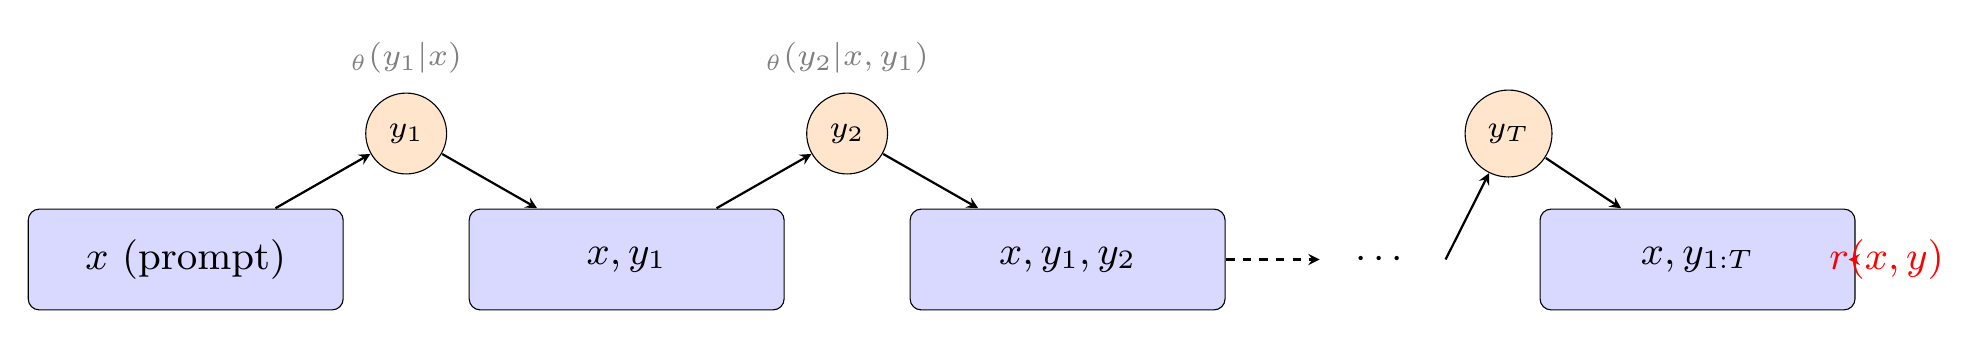
\begin{tikzpicture}[
        state/.style={draw, rounded corners, fill=blue!15, minimum width=2.5cm, minimum height=0.8cm, align=center, font=\small},
        action/.style={circle, draw, fill=orange!20, minimum size=0.6cm, font=\scriptsize},
        arrow/.style={->, thick, >=stealth}
    ]
        % 状态序列
        \node[state] (s0) at (0, 0) {$x$ (prompt)};
        \node[state] (s1) at (3.5, 0) {$x, y_1$};
        \node[state] (s2) at (7, 0) {$x, y_1, y_2$};
        \node[font=\small] at (9.5, 0) {$\cdots$};
        \node[state] (sT) at (12, 0) {$x, y_{1:T}$};

        % 动作
        \node[action] (a1) at (1.75, 1) {$y_1$};
        \node[action] (a2) at (5.25, 1) {$y_2$};
        \node[action] (aT) at (10.5, 1) {$y_T$};

        % 奖励
        \node[font=\small, red] at (13.5, 0) {$r(x, y)$};

        % 连接
        \draw[arrow] (s0) -- (a1);
        \draw[arrow] (a1) -- (s1);
        \draw[arrow] (s1) -- (a2);
        \draw[arrow] (a2) -- (s2);
        \draw[arrow, dashed] (s2) -- (9, 0);
        \draw[arrow] (10, 0) -- (aT);
        \draw[arrow] (aT) -- (sT);
        \draw[arrow, red] (sT) -- (13.2, 0);

        % 标注
        \node[font=\scriptsize, gray] at (1.75, 1.6) {$\policy_\theta(y_1|x)$};
        \node[font=\scriptsize, gray] at (5.25, 1.6) {$\policy_\theta(y_2|x,y_1)$};
    \end{tikzpicture}
    \caption{LLM 生成过程的 MDP 建模}
    \label{fig:llm-mdp}
\end{figure}

LLM RL 的特点:
\begin{itemize}
    \item \textbf{动作空间巨大}:词表通常有 10 万+ token
    \item \textbf{确定性状态转移}:下一状态 = 当前状态 + 新 token
    \item \textbf{Episode = 一次完整生成}:从 prompt 到 EOS
    \item \textbf{稀疏奖励}:只有序列结束时才有奖励信号
\end{itemize}

\subsection{稀疏奖励问题}

LLM 对齐的典型奖励结构:
\begin{equation}
    r_t = \begin{cases}
        0 & t < T \\
        r_\phi(x, y) & t = T \text{(序列结束)}
    \end{cases}
\end{equation}

稀疏奖励带来的挑战:
\begin{itemize}
    \item \textbf{信用分配困难}:最终奖励如何归因到每个 token?
    \item \textbf{梯度信号弱}:大部分时刻没有学习信号
    \item \textbf{长序列尤其困难}:信号需要传播很远(数千 token)
\end{itemize}

\begin{note}
解决稀疏奖励的两种思路:
\begin{enumerate}
    \item \textbf{序列级方法}:把整个序列当作一个 bandit,用序列奖励直接更新(如 REINFORCE)
    \item \textbf{过程奖励}:训练 PRM 提供中间步骤的奖励信号
\end{enumerate}
\end{note}

% ------------------------------------------
\section{RLHF 三阶段}
\label{sec:rlhf}

RLHF(Reinforcement Learning from Human Feedback)是 LLM 对齐的经典方法,由 OpenAI 在 InstructGPT 中系统化。

\subsection{RLHF 整体架构}

\begin{figure}[H]
    \centering
    \begin{tikzpicture}[scale=0.9, every node/.style={scale=0.9},
        box/.style={draw, rounded corners, minimum width=2.8cm, minimum height=1cm, align=center},
        data/.style={draw, rounded corners, fill=gray!15, minimum width=2cm, minimum height=0.8cm, align=center, font=\small},
        arrow/.style={->, thick, >=stealth}
    ]
        % Stage 1
        \begin{scope}[shift={(-5, 0)}]
            \node[box, fill=blue!20] (pt) at (0, 2) {预训练模型};
            \node[data] (sft_data) at (0, 0) {高质量对话\\数据};
            \node[box, fill=green!20] (sft) at (0, -2) {SFT 模型\\$\policy_{\text{ref}}$};

            \draw[arrow] (pt) -- (sft);
            \draw[arrow] (sft_data) -- (sft);

            \node[font=\bfseries] at (0, 3.5) {Stage 1: SFT};
        \end{scope}

        % Stage 2
        \begin{scope}[shift={(0, 0)}]
            \node[box, fill=green!15] (sft2) at (0, 2) {SFT 模型};
            \node[data] (pref_data) at (0, 0) {人类偏好数据\\$(x, y_w, y_l)$};
            \node[box, fill=orange!20] (rm) at (0, -2) {Reward Model\\$r_\phi(x, y)$};

            \draw[arrow] (sft2) -- (rm);
            \draw[arrow] (pref_data) -- (rm);

            \node[font=\bfseries] at (0, 3.5) {Stage 2: RM};
        \end{scope}

        % Stage 3
        \begin{scope}[shift={(5.5, 0)}]
            \node[box, fill=green!15] (ref) at (-1.8, 2) {$\policy_{\text{ref}}$};
            \node[box, fill=orange!15] (rm2) at (1.8, 2) {$r_\phi$};
            \node[box, fill=purple!20] (ppo) at (0, 0) {PPO 训练};
            \node[box, fill=red!20] (final) at (0, -2) {对齐模型\\$\policy_\theta$};

            \draw[arrow] (ref) -- (ppo);
            \draw[arrow] (rm2) -- (ppo);
            \draw[arrow] (ppo) -- (final);

            \node[font=\bfseries] at (0, 3.5) {Stage 3: PPO};
        \end{scope}

        % 连接箭头
        \draw[arrow, dashed, gray] (-3, -2) -- (-2, 2);
        \draw[arrow, dashed, gray] (2, -2) -- (4, 2);
    \end{tikzpicture}
    \caption{RLHF 三阶段架构}
    \label{fig:rlhf-pipeline}
\end{figure}

\subsection{Stage 1: Supervised Fine-Tuning (SFT)}

用高质量对话数据微调预训练模型:
\begin{equation}
    L_{\text{SFT}}(\theta) = -\E_{(x,y) \sim \mathcal{D}_{\text{SFT}}} \left[ \log \policy_\theta(y|x) \right] = -\E \left[ \sum_{t=1}^{T} \log \policy_\theta(y_t | x, y_{<t}) \right]
\end{equation}

SFT 的作用:
\begin{itemize}
    \item 让模型学会"指令遵循"的基本格式
    \item 提供 RL 的起点(参考模型 $\policy_{\text{ref}}$)
    \item 过滤预训练中的低质量模式
\end{itemize}

\subsection{Stage 2: Reward Model 训练}

从人类偏好数据中学习 Reward Model。

\begin{definition}[偏好数据]
对于 prompt $x$,人类标注者比较两个回复,给出偏好:$y_w \succ y_l$($y_w$ 优于 $y_l$)。
\end{definition}

\subsubsection{Bradley-Terry 模型}

\begin{definition}[Bradley-Terry 模型]
假设人类偏好遵循 Bradley-Terry 模型——偏好概率由"能力差"决定:
\begin{equation}
    P(y_w \succ y_l | x) = \sigma(r(x, y_w) - r(x, y_l)) = \frac{1}{1 + e^{-(r(x, y_w) - r(x, y_l))}}
    \label{eq:bradley-terry}
\end{equation}
其中 $\sigma(z) = \frac{1}{1+e^{-z}}$ 是 sigmoid 函数,$r(x, y)$ 是回复的"得分"。
\end{definition}

\begin{figure}[H]
    \centering
    \begin{tikzpicture}
        \begin{axis}[
            width=10cm, height=5cm,
            xlabel={$r(y_w) - r(y_l)$(奖励差)},
            ylabel={$P(y_w \succ y_l)$(偏好概率)},
            domain=-6:6,
            samples=100,
            grid=major,
            ymin=0, ymax=1
        ]
            \addplot[thick, blue] {1/(1+exp(-x))};
            \draw[dashed, gray] (axis cs:0, 0.5) -- (axis cs:0, 0);
            \node[font=\small] at (axis cs:3, 0.3) {奖励差越大};
            \node[font=\small] at (axis cs:3, 0.2) {偏好越确定};
        \end{axis}
    \end{tikzpicture}
    \caption{Bradley-Terry 模型:偏好概率由奖励差决定}
    \label{fig:bradley-terry}
\end{figure}

Bradley-Terry 模型的直觉:
\begin{itemize}
    \item 奖励差 = 0 时,偏好概率 = 0.5(无法区分)
    \item 奖励差越大,偏好概率越接近 1(更确定)
    \item 模型假设偏好是基于"内在质量分数"的概率比较
\end{itemize}

\subsubsection{Reward Model 训练}

Reward Model 的训练目标是最大化偏好数据的似然:
\begin{equation}
    L_{\text{RM}}(\phi) = -\E_{(x, y_w, y_l)} \left[ \log \sigma(r_\phi(x, y_w) - r_\phi(x, y_l)) \right]
    \label{eq:rm-loss}
\end{equation}

这是一个\textbf{二分类问题}:给定 $(y_w, y_l)$,预测哪个更好。

\begin{note}
Reward Model 的架构选择:
\begin{itemize}
    \item 通常用 SFT 模型初始化
    \item 去掉语言模型头,加上标量输出头
    \item 输入 $(x, y)$,输出标量 $r_\phi(x, y) \in \R$
\end{itemize}
\end{note}

\subsection{Stage 3: PPO 微调}

使用 Reward Model 提供奖励信号,用 PPO 优化策略。

\begin{definition}[RLHF 优化目标]
\begin{equation}
    \max_\theta \E_{x \sim \mathcal{D}, y \sim \policy_\theta(\cdot|x)} \left[ r_\phi(x, y) \right] - \beta \cdot \text{KL}(\policy_\theta \| \policy_{\text{ref}})
    \label{eq:rlhf-objective}
\end{equation}
其中 $\beta > 0$ 是 KL 正则系数。
\end{definition}

\subsubsection{KL 正则的作用}

KL 正则项 $\text{KL}(\policy_\theta \| \policy_{\text{ref}})$ 至关重要:

\begin{enumerate}
    \item \textbf{防止 Reward Hacking}:
    \begin{itemize}
        \item Reward Model 是不完美的代理
        \item 无约束优化会找到"欺骗" RM 的方式
        \item 例如:生成特定模式获得高分,但实际质量差
    \end{itemize}

    \item \textbf{保持生成质量}:
    \begin{itemize}
        \item SFT 模型已经有较好的语言能力
        \item KL 约束防止偏离太远导致流利度下降
    \end{itemize}

    \item \textbf{稳定训练}:
    \begin{itemize}
        \item 约束优化空间,避免策略崩溃
        \item 提供正则化效果
    \end{itemize}
\end{enumerate}

\begin{figure}[H]
    \centering
    \begin{tikzpicture}[
        arrow/.style={->, thick, >=stealth}
    ]
        % 坐标轴
        \draw[arrow] (-0.5, 0) -- (8, 0) node[right] {$\text{KL}(\policy_\theta \| \policy_{\text{ref}})$};
        \draw[arrow] (0, -0.5) -- (0, 5) node[above] {$\E[r_\phi]$};

        % 曲线
        \draw[thick, blue, domain=0.2:7, samples=100] plot (\x, {4 - 0.8*(\x-3)^2/9 + 0.5*ln(\x)});

        % 最优点
        \fill[red] (2.5, 3.8) circle (3pt);
        \node[font=\small, red] at (2.5, 4.3) {最优权衡};

        % 区域标注
        \node[font=\scriptsize, align=center] at (1, 2) {KL 太小\\改进有限};
        \node[font=\scriptsize, align=center] at (6, 2) {KL 太大\\Reward Hacking};

        % beta 的作用
        \draw[dashed, gray] (0, 3.8) -- (2.5, 3.8) -- (2.5, 0);
    \end{tikzpicture}
    \caption{KL 正则的权衡:$\beta$ 控制在 reward 和 KL 之间的平衡点}
    \label{fig:kl-tradeoff}
\end{figure}

\subsubsection{PPO 更新流程}

RLHF 中 PPO 的具体步骤:

\begin{algorithm}[H]
\caption{RLHF with PPO}
\label{alg:rlhf-ppo}
\KwInput{SFT 模型 $\policy_{\text{ref}}$,Reward Model $r_\phi$,KL 系数 $\beta$}
初始化 $\policy_\theta \leftarrow \policy_{\text{ref}}$,Critic $\Val_\psi$\;
\ForEach{iteration}{
    \tcp{采样}
    从 prompt 分布采样 $x \sim \mathcal{D}$\;
    用当前策略生成回复 $y \sim \policy_\theta(\cdot|x)$\;

    \tcp{计算奖励}
    计算 RM 奖励:$r^{\text{RM}} = r_\phi(x, y)$\;
    计算 KL 惩罚:$r^{\text{KL}}_t = -\beta \log \frac{\policy_\theta(y_t|x, y_{<t})}{\policy_{\text{ref}}(y_t|x, y_{<t})}$\;
    总奖励:$r_t = r^{\text{KL}}_t + \ind_{t=T} \cdot r^{\text{RM}}$\;

    \tcp{GAE 计算}
    用 Critic $\Val_\psi$ 计算 advantage $\hat{\advantage}_t$\;

    \tcp{PPO 更新}
    用 PPO-Clip 目标更新 $\policy_\theta$\;
    用 TD 目标更新 $\Val_\psi$\;
}
\end{algorithm}

\begin{important}
RLHF 需要维护的模型:
\begin{enumerate}
    \item $\policy_\theta$:正在训练的策略(Active Model)
    \item $\policy_{\text{ref}}$:参考模型(冻结)
    \item $r_\phi$:Reward Model(冻结)
    \item $\Val_\psi$:Critic 网络
\end{enumerate}
共 4 个大模型,显存开销巨大!这是 DPO、GRPO 等方法试图解决的问题。
\end{important}

% ------------------------------------------
\section{Direct Preference Optimization (DPO)}
\label{sec:dpo}

DPO 是一种绕过 Reward Model 和 PPO 的简化方法,由 Rafailov et al. 2023 提出。

\subsection{DPO 的动机}

RLHF + PPO 的问题:
\begin{itemize}
    \item \textbf{模型开销大}:需要维护 4 个模型
    \item \textbf{采样成本高}:大模型在线生成很贵
    \item \textbf{实现复杂}:PPO 超参敏感,需要精细调参
    \item \textbf{训练不稳定}:RL 训练容易崩溃
\end{itemize}

\begin{quote}
\textbf{DPO 的核心问题}:能否直接在偏好数据 $(x, y_w, y_l)$ 上优化,像监督学习一样简单?
\end{quote}

答案是可以的!关键洞察:KL 正则的 RL 问题有\textbf{闭式解}。

\subsection{DPO Loss 公式}

\begin{definition}[DPO Loss]
\begin{equation}
    L_{\text{DPO}}(\theta) = -\E_{(x, y_w, y_l)} \left[ \log \sigma \left( \beta \left[ \log \frac{\policy_\theta(y_w|x)}{\policy_{\text{ref}}(y_w|x)} - \log \frac{\policy_\theta(y_l|x)}{\policy_{\text{ref}}(y_l|x)} \right] \right) \right]
    \label{eq:dpo-loss}
\end{equation}
\end{definition}

\subsection{DPO 完整推导}

\begin{theorem}[DPO 等价性]
DPO Loss \eqref{eq:dpo-loss} 与 RLHF 目标 \eqref{eq:rlhf-objective} 在最优解处等价。
\end{theorem}

\begin{proof}
推导分为 5 个关键步骤。

\textbf{Step 1:RLHF 目标展开}

RLHF 优化目标:
\begin{equation}
    \max_\policy \E_{y \sim \policy} \left[ r(x, y) \right] - \beta \cdot \text{KL}(\policy \| \policy_{\text{ref}})
\end{equation}

展开 KL 散度:
\begin{align}
    &= \E_{y \sim \policy} \left[ r(x, y) \right] - \beta \E_{y \sim \policy} \left[ \log \frac{\policy(y|x)}{\policy_{\text{ref}}(y|x)} \right] \\
    &= \E_{y \sim \policy} \left[ r(x, y) - \beta \log \frac{\policy(y|x)}{\policy_{\text{ref}}(y|x)} \right]
\end{align}

\textbf{Step 2:引入配分函数 $Z(x)$}

为了让最优策略是合法的概率分布,定义配分函数:
\begin{equation}
    Z(x) = \sum_y \policy_{\text{ref}}(y|x) \exp\left( \frac{r(x,y)}{\beta} \right)
\end{equation}

$Z(x)$ 是归一化常数,只依赖于 $x$(不依赖于被优化的策略)。

\textbf{Step 3:最优策略的闭式解}

KL 正则 RL 问题有闭式解:

\begin{lemma}[KL 正则 RL 的最优策略]
目标 $\max_\policy \E_{y \sim \policy}[r(y)] - \beta \cdot \text{KL}(\policy \| \policy_{\text{ref}})$ 的最优解为:
\begin{equation}
    \policy^*(y|x) = \frac{1}{Z(x)} \policy_{\text{ref}}(y|x) \exp\left( \frac{r(x,y)}{\beta} \right)
    \label{eq:optimal-policy-kl}
\end{equation}
\end{lemma}

\begin{proof}
这是一个有约束优化问题($\policy$ 需要是概率分布)。用拉格朗日乘子法或变分推断可得。
直觉:最优策略是参考策略按 $\exp(r/\beta)$ 重新加权。奖励越高,概率提升越多。
\end{proof}

\textbf{Step 4:从最优策略反解 reward}

关键步骤:从 \eqref{eq:optimal-policy-kl} 反解 reward。

取对数:
\begin{align}
    \log \policy^*(y|x) &= \log \policy_{\text{ref}}(y|x) - \log Z(x) + \frac{r(x,y)}{\beta}
\end{align}

整理得:
\begin{equation}
    r(x,y) = \beta \log \frac{\policy^*(y|x)}{\policy_{\text{ref}}(y|x)} + \beta \log Z(x)
    \label{eq:reward-from-policy}
\end{equation}

\begin{keypoint}
核心洞察:reward 可以用策略的 log-ratio 表示!虽然有 $\log Z(x)$ 项,但它只依赖于 $x$,在 pairwise 比较中会消除。
\end{keypoint}

\textbf{Step 5:代入 Bradley-Terry 模型,$Z(x)$ 消除}

将 \eqref{eq:reward-from-policy} 代入 Bradley-Terry 模型 \eqref{eq:bradley-terry}:
\begin{align}
    P(y_w \succ y_l) &= \sigma(r(x, y_w) - r(x, y_l)) \\
    &= \sigma\bigg( \underbrace{\beta \log \frac{\policy^*(y_w|x)}{\policy_{\text{ref}}(y_w|x)} + \beta \log Z(x)}_{r(x, y_w)} - \underbrace{\beta \log \frac{\policy^*(y_l|x)}{\policy_{\text{ref}}(y_l|x)} - \beta \log Z(x)}_{r(x, y_l)} \bigg) \\
    &= \sigma\left( \beta \left[ \log \frac{\policy^*(y_w|x)}{\policy_{\text{ref}}(y_w|x)} - \log \frac{\policy^*(y_l|x)}{\policy_{\text{ref}}(y_l|x)} \right] \right)
\end{align}

$\beta \log Z(x)$ 项相消了!

最大化偏好数据的 log-likelihood,用 $\policy_\theta$ 代替 $\policy^*$,得到 DPO Loss:
\begin{equation}
    L_{\text{DPO}}(\theta) = -\E \left[ \log \sigma \left( \beta \left[ \log \frac{\policy_\theta(y_w|x)}{\policy_{\text{ref}}(y_w|x)} - \log \frac{\policy_\theta(y_l|x)}{\policy_{\text{ref}}(y_l|x)} \right] \right) \right]
\end{equation}
\end{proof}

\begin{figure}[H]
    \centering
    \begin{tikzpicture}[
        box/.style={draw, rounded corners, fill=blue!10, minimum width=3.5cm, minimum height=1cm, align=center},
        arrow/.style={->, thick, >=stealth}
    ]
        \node[box] (rlhf) at (0, 3) {RLHF 目标\\$\max \E[r] - \beta \cdot \text{KL}$};
        \node[box] (opt) at (0, 1) {最优策略闭式解\\$\policy^* \propto \policy_{\text{ref}} \exp(r/\beta)$};
        \node[box] (reward) at (0, -1) {反解 reward\\$r = \beta \log \frac{\policy^*}{\policy_{\text{ref}}} + \beta \log Z$};
        \node[box, fill=green!20] (dpo) at (0, -3) {DPO Loss\\$Z(x)$ 消除};

        \draw[arrow] (rlhf) -- node[right, font=\small] {KL-RL 闭式解} (opt);
        \draw[arrow] (opt) -- node[right, font=\small] {取对数} (reward);
        \draw[arrow] (reward) -- node[right, font=\small] {代入 BT 模型} (dpo);
    \end{tikzpicture}
    \caption{DPO 推导的逻辑链条}
    \label{fig:dpo-derivation}
\end{figure}

\begin{important}
DPO 的核心洞察:
\begin{enumerate}
    \item KL 正则 RL 问题有闭式解,最优策略是参考策略的指数重加权
    \item 可以从最优策略反解隐式 reward
    \item 配分函数 $Z(x)$ 在 pairwise 比较中消除——这是 DPO 能 work 的关键
    \item 最终形式只需要计算 log-probability,像监督学习一样简单
\end{enumerate}
\end{important}

\subsection{DPO 的直观理解}

定义 \textbf{隐式奖励}:
\begin{equation}
    \hat{r}_\theta(x, y) = \beta \log \frac{\policy_\theta(y|x)}{\policy_{\text{ref}}(y|x)}
\end{equation}

DPO Loss 可以写成:
\begin{equation}
    L_{\text{DPO}} = -\E \left[ \log \sigma(\hat{r}_\theta(x, y_w) - \hat{r}_\theta(x, y_l)) \right]
\end{equation}

直觉:
\begin{itemize}
    \item $\hat{r}_\theta(x, y_w) > \hat{r}_\theta(x, y_l)$:$y_w$ 的隐式奖励更高,loss 变小
    \item 训练过程提高 $y_w$ 相对于 $\policy_{\text{ref}}$ 的概率,压低 $y_l$ 的概率
    \item $\beta$ 控制"相对于参考策略偏离多少"的尺度
\end{itemize}

\subsection{DPO vs RLHF 对比}

\begin{table}[H]
    \centering
    \begin{tabular}{@{}lcc@{}}
        \toprule
        & \textbf{RLHF + PPO} & \textbf{DPO} \\
        \midrule
        需要 Reward Model & 是 & 否 \\
        需要 Critic 网络 & 是 & 否 \\
        训练方式 & 在线采样 & 离线训练 \\
        模型数量 & 4 个 & 2 个 \\
        实现复杂度 & 高 & 低 \\
        超参敏感性 & 高 & 低 \\
        探索能力 & 有 & 无 \\
        适用场景 & 复杂任务 & 简单对齐 \\
        \bottomrule
    \end{tabular}
    \caption{RLHF + PPO 与 DPO 的对比}
\end{table}

DPO 的局限:
\begin{itemize}
    \item \textbf{无探索}:完全离线,只能在已有偏好数据的分布内优化
    \item \textbf{Pairwise 信号粗糙}:只知道谁更好,不知道好多少
    \item \textbf{难任务提升有限}:在数学、代码等需要探索的任务上效果不如 RL
\end{itemize}

% ------------------------------------------
\section{GRPO:Group Relative Policy Optimization}
\label{sec:grpo}

GRPO 是 DeepSeek 提出的方法,介于 PPO 和 DPO 之间:保留在线探索能力,但不需要 Critic 网络。

\subsection{GRPO 的动机}

\begin{itemize}
    \item \textbf{PPO 的问题}:需要 Critic 网络,显存开销大(额外一个大模型)
    \item \textbf{DPO 的问题}:完全离线,缺乏探索,难任务提升有限
\end{itemize}

GRPO 的思路:\textbf{用组内相对奖励代替 Critic},实现"无 Critic 的在线 RL"。

\subsection{组内标准化 Advantage}

\begin{definition}[GRPO Advantage]
对于 prompt $x$,采样一组回复 $\{y_1, \ldots, y_G\}$,计算各自的奖励 $\{R_1, \ldots, R_G\}$,然后:
\begin{equation}
    \hat{\advantage}_i = \frac{R_i - \bar{R}}{\text{Std}(R) + \epsilon}
    \label{eq:grpo-advantage}
\end{equation}
其中 $\bar{R} = \frac{1}{G}\sum_i R_i$ 是组内均值,$\text{Std}(R)$ 是组内标准差。
\end{definition}

\begin{figure}[H]
    \centering
    \begin{tikzpicture}[
        sample/.style={circle, draw, minimum size=0.6cm, font=\scriptsize},
        arrow/.style={->, thick, >=stealth}
    ]
        % Prompt
        \node[draw, rounded corners, fill=blue!20, minimum width=2cm] (prompt) at (0, 0) {Prompt $x$};

        % 生成多个回复
        \node[sample, fill=green!30] (y1) at (3, 1.5) {$y_1$};
        \node[sample, fill=green!20] (y2) at (3, 0.5) {$y_2$};
        \node[sample, fill=red!20] (y3) at (3, -0.5) {$y_3$};
        \node[sample, fill=red!30] (y4) at (3, -1.5) {$y_4$};

        \draw[arrow] (prompt) -- (y1);
        \draw[arrow] (prompt) -- (y2);
        \draw[arrow] (prompt) -- (y3);
        \draw[arrow] (prompt) -- (y4);

        % 奖励
        \node[font=\scriptsize] at (4.5, 1.5) {$R_1 = 0.8$};
        \node[font=\scriptsize] at (4.5, 0.5) {$R_2 = 0.6$};
        \node[font=\scriptsize] at (4.5, -0.5) {$R_3 = 0.3$};
        \node[font=\scriptsize] at (4.5, -1.5) {$R_4 = 0.1$};

        % 标准化
        \node[font=\small] at (7, 0) {$\bar{R} = 0.45$};

        % Advantage
        \node[font=\scriptsize, green!60!black] at (9, 1.5) {$\hat{A}_1 > 0$};
        \node[font=\scriptsize, green!60!black] at (9, 0.5) {$\hat{A}_2 > 0$};
        \node[font=\scriptsize, red] at (9, -0.5) {$\hat{A}_3 < 0$};
        \node[font=\scriptsize, red] at (9, -1.5) {$\hat{A}_4 < 0$};

        % 说明
        \node[font=\small, align=center] at (5, -3) {组内相对比较:\\高于均值的增强,低于均值的抑制};
    \end{tikzpicture}
    \caption{GRPO 组内标准化示意图}
    \label{fig:grpo-advantage}
\end{figure}

组内标准化的优势:
\begin{enumerate}
    \item \textbf{无需 Critic}:用组内均值代替价值函数估计
    \item \textbf{Baseline 效果}:均值减法降低方差
    \item \textbf{尺度归一化}:标准差归一化使 advantage 尺度稳定
    \item \textbf{相对比较}:focus 在同一 prompt 下的相对好坏
\end{enumerate}

\subsection{GRPO 目标函数}

\begin{definition}[GRPO 目标]
\begin{equation}
    L_{\text{GRPO}} = \E_{x} \left[ \frac{1}{G} \sum_{i=1}^{G} \sum_{t=1}^{|y_i|} \min \left( \rho_{i,t} \hat{\advantage}_i, \text{clip}(\rho_{i,t}, 1-\epsilon, 1+\epsilon) \hat{\advantage}_i \right) \right]
\end{equation}
其中 $\rho_{i,t} = \frac{\policy_\theta(y_{i,t}|x, y_{i,<t})}{\policy_{\theta_{\text{old}}}(y_{i,t}|x, y_{i,<t})}$ 是 importance sampling 比率。
\end{definition}

\begin{note}
GRPO 与 PPO 的关键区别:
\begin{itemize}
    \item PPO:$\hat{\advantage}_t$ 由 GAE 计算,需要 Critic
    \item GRPO:$\hat{\advantage}_i$ 对整个序列恒定,由组内标准化得到
\end{itemize}
\end{note}

\subsection{GRPO 实用技巧}

\begin{enumerate}
    \item \textbf{Clip-Higher}:上界可以更宽松(如 $1+0.28$ 而非 $1+0.2$),允许好回复更大幅度提升

    \item \textbf{Dynamic Sampling}:过滤全对或全错的 prompt(方差为 0 时 advantage 无定义)

    \item \textbf{长度惩罚}:防止生成过长的回复
    \begin{equation}
        R_i = r_\phi(x, y_i) - \lambda \cdot |y_i|
    \end{equation}

    \item \textbf{KL as Loss}:KL 惩罚作为独立 loss 项,而非放入 reward
    \begin{equation}
        L = -L_{\text{GRPO}} + \lambda_{\text{KL}} \cdot \E[\text{KL}(\policy_\theta \| \policy_{\text{ref}})]
    \end{equation}
\end{enumerate}

% ------------------------------------------
\section{KL 散度估计:k1, k2, k3}
\label{sec:kl-estimators}

KL 散度 $\text{KL}(\policy_\theta \| \policy_{\text{ref}})$ 无法精确计算(需要遍历所有可能的序列),需要蒙特卡洛估计。

\subsection{KL 散度的定义}

对于两个分布 $p$ 和 $q$:
\begin{equation}
    \text{KL}(p \| q) = \E_{x \sim p}\left[ \log \frac{p(x)}{q(x)} \right]
\end{equation}

在 LLM 场景中,$p = \policy_\theta$,$q = \policy_{\text{ref}}$,从 $\policy_\theta$ 采样。

\subsection{k1 估计器:直接估计}

\begin{definition}[k1 估计器]
定义比率 $r = \frac{\policy_{\text{ref}}(y|x)}{\policy_\theta(y|x)}$,则:
\begin{equation}
    k_1 = -\log r = \log \frac{\policy_\theta(y|x)}{\policy_{\text{ref}}(y|x)}
\end{equation}
\end{definition}

性质:
\begin{itemize}
    \item \textbf{无偏}:$\E_{y \sim \policy_\theta}[k_1] = \text{KL}(\policy_\theta \| \policy_{\text{ref}})$
    \item \textbf{高方差}:当 $\policy_\theta$ 和 $\policy_{\text{ref}}$ 差异大时,方差很大
\end{itemize}

用法:通常放入 reward
\begin{equation}
    r_t^{\text{RL}} = r_t^{\text{RM}} - \beta \cdot k_1^{(t)}
\end{equation}

\subsection{k2 估计器:平方形式}

\begin{definition}[k2 估计器]
\begin{equation}
    k_2 = \frac{1}{2}(\log r)^2 = \frac{1}{2} \left( \log \frac{\policy_{\text{ref}}(y|x)}{\policy_\theta(y|x)} \right)^2
\end{equation}
\end{definition}

性质:
\begin{itemize}
    \item \textbf{有偏}:$\E[k_2] \neq \text{KL}$
    \item \textbf{梯度等价}:$\nabla_\theta \E[k_2] = \nabla_\theta \text{KL}$
    \item \textbf{更平滑}:平方形式在 $r=1$ 附近更平滑
\end{itemize}

用法:适合作为 loss 项(因为梯度正确)

\subsection{k3 估计器:Control Variate}

\begin{definition}[k3 估计器]
\begin{equation}
    k_3 = (r - 1) - \log r = \frac{\policy_{\text{ref}}(y|x)}{\policy_\theta(y|x)} - 1 - \log \frac{\policy_{\text{ref}}(y|x)}{\policy_\theta(y|x)}
\end{equation}
\end{definition}

\begin{theorem}[k3 的性质]
k3 是无偏且低方差的 KL 估计器。
\end{theorem}

\begin{proof}
无偏性:
\begin{align}
    \E_{y \sim \policy_\theta}[k_3] &= \E[(r-1)] - \E[\log r] \\
    &= \underbrace{\E\left[\frac{\policy_{\text{ref}}}{\policy_\theta}\right] - 1}_{= 0} + \E\left[\log \frac{\policy_\theta}{\policy_{\text{ref}}}\right] \\
    &= \text{KL}(\policy_\theta \| \policy_{\text{ref}})
\end{align}

其中 $\E_{y \sim \policy_\theta}\left[\frac{\policy_{\text{ref}}(y)}{\policy_\theta(y)}\right] = \sum_y \policy_\theta(y) \cdot \frac{\policy_{\text{ref}}(y)}{\policy_\theta(y)} = \sum_y \policy_{\text{ref}}(y) = 1$。

低方差:$(r-1)$ 项是一个 control variate,期望为 0,与 $\log r$ 负相关,减少方差。
\end{proof}

\subsection{三种估计器对比}

\begin{table}[H]
    \centering
    \begin{tabular}{@{}lcccc@{}}
        \toprule
        估计器 & 公式 & 偏差 & 方差 & 推荐用法 \\
        \midrule
        k1 & $\log \frac{\policy_\theta}{\policy_{\text{ref}}}$ & 无偏 & 高 & KL in reward \\
        k2 & $\frac{1}{2}(\log \frac{\policy_{\text{ref}}}{\policy_\theta})^2$ & 有偏 & 低 & KL as loss \\
        k3 & $\frac{\policy_{\text{ref}}}{\policy_\theta} - 1 - \log \frac{\policy_{\text{ref}}}{\policy_\theta}$ & 无偏 & 低 & KL as loss \\
        \bottomrule
    \end{tabular}
    \caption{KL 估计器对比}
\end{table}

\begin{keypoint}
KL 的两种用法:
\begin{enumerate}
    \item \textbf{KL in Reward}(经典 RLHF):
    \begin{itemize}
        \item Token reward 减去 $\beta \cdot k_1$
        \item 然后用 PPO-Clip 更新
        \item 优点:直接影响每步决策
    \end{itemize}

    \item \textbf{KL as Loss}(GRPO 等):
    \begin{itemize}
        \item 总 loss = $-L_{\text{RL}} + \lambda \cdot \E[k_3]$
        \item 优点:更稳定,方差更低
    \end{itemize}
\end{enumerate}
\end{keypoint}

% ------------------------------------------
\section{On-Policy Distillation}
\label{sec:on-policy-distillation}

On-Policy Distillation 是近年来 LLM 后训练的重要进展,由 GKD~\cite{agarwal2024gkd} 和 MiniLLM~\cite{gu2024minillm} 等工作奠定基础,并在 Qwen3~\cite{yang2025qwen3} 等前沿模型中得到成功应用。

\subsection{动机:Off-policy 蒸馏的分布偏移问题}

传统的知识蒸馏(SFT on 教师数据)是 \textbf{off-policy} 的:

\begin{quote}
\textbf{学生从教师生成的数据学习,但推理时走到的状态可能与训练时完全不同。}
\end{quote}

这导致 \textbf{compounding errors}——学生在训练时没见过自己犯的错误,一旦偏离教师轨迹就会持续恶化。尤其在长序列推理任务中,这种分布偏移问题更为严重。

\begin{itemize}
    \item \textbf{Off-policy SFT}:密集监督,但分布偏移
    \item \textbf{On-policy RL}:分布匹配,但奖励稀疏、效率低
\end{itemize}

自然的问题:能否结合两者优势——在学生自己的分布上获得密集监督?

\subsection{三种后训练范式对比}

\begin{table}[H]
    \centering
    \begin{tabular}{@{}lccc@{}}
        \toprule
        方法 & 采样来源 & 奖励密度 & 特点 \\
        \midrule
        SFT(监督微调) & 教师数据(Off-policy) & 密集 & 分布受限 \\
        RL(强化学习) & 自身采样(On-policy) & 稀疏 & 搜索成本高 \\
        On-Policy Distillation & \textbf{自身采样} & \textbf{密集} & 两者优势结合 \\
        \bottomrule
    \end{tabular}
    \caption{三种后训练范式对比}
    \label{tab:post-training-paradigms}
\end{table}

On-Policy Distillation 的核心思想:
\begin{itemize}
    \item \textbf{学生自己采样}(On-policy):避免分布偏移
    \item \textbf{教师逐 token 打分}(Dense reward):提供密集监督信号
\end{itemize}

\subsection{Reverse KL 损失}

On-Policy Distillation 使用 \textbf{反向 KL 散度}作为损失函数:
\begin{equation}
    L_{\text{OPD}} = D_{\text{KL}}(\policy_\theta \| \policy_{\text{teacher}}) = \E_{y \sim \policy_\theta}\left[ \sum_t \log \frac{\policy_\theta(y_t | x, y_{<t})}{\policy_{\text{teacher}}(y_t | x, y_{<t})} \right]
\end{equation}

\begin{note}
\textbf{Forward KL vs Reverse KL}:
\begin{itemize}
    \item Forward KL $D_{\text{KL}}(\policy_{\text{teacher}} \| \policy_\theta)$:mode covering,学生试图覆盖教师的所有模式
    \item Reverse KL $D_{\text{KL}}(\policy_\theta \| \policy_{\text{teacher}})$:mode seeking,学生专注于教师的高概率区域
\end{itemize}
Reverse KL 更适合蒸馏场景——让学生在自己访问的状态上模仿教师,而非试图覆盖教师的全部行为。
\end{note}

\subsection{KDRL:结合知识蒸馏与强化学习}

KDRL~\cite{xu2025kdrl}(Knowledge Distillation + Reinforcement Learning)将教师监督和奖励驱动的自我探索统一为联合优化:

\begin{equation}
    \mathcal{J}_{\text{KDRL}}(\theta) = \underbrace{\mathcal{J}_{\text{GRPO}}(\theta)}_{\text{奖励驱动}} - \beta \cdot \underbrace{D_{\text{KL}}^{k_2}(\policy_\theta \| \policy_{\text{teacher}})}_{\text{教师监督}}
\end{equation}

关键设计选择:
\begin{enumerate}
    \item \textbf{KL 估计器选择}:$k_2$ 优于 $k_3$,因为 $k_2$ 提供无偏梯度估计
    \item \textbf{系数退火}:从强模仿($\beta$ 大)逐渐过渡到奖励驱动($\beta$ 小)
    \item \textbf{奖励引导 Masking}:只在低奖励样本上应用 KD,减少输出长度同时保持准确率
\end{enumerate}

\subsection{效率优势}

\begin{keypoint}
On-Policy Distillation 的效率提升(以数学推理任务为例):
\begin{itemize}
    \item 相比 RL:训练速度快 7-10 倍,总计算效率提升 50-100 倍
    \item 相比离线蒸馏:计算成本降低 9-30 倍
    \item Qwen3 实验:蒸馏显著优于 RL,GPU 小时仅需 RL 的约 1/10
\end{itemize}
\end{keypoint}

效率提升的根本原因:
\begin{quote}
\textbf{教师提供的密集 token 级信号,比 RL 的稀疏序列级奖励包含更多信息。}

RL 的大部分计算花在搜索(探索策略空间),蒸馏则直接利用教师的知识指导学生在关键"分叉点"做出正确选择。
\end{quote}

\subsection{应用场景}

\begin{enumerate}
    \item \textbf{小模型专业化}:用大模型(如 Qwen3-235B)蒸馏小模型(如 Qwen3-32B)
    \item \textbf{持续学习}:新领域知识训练后,用蒸馏恢复遗忘的指令遵循能力
    \item \textbf{行为恢复}:从早期 checkpoint 恢复特定能力
\end{enumerate}

\begin{important}
\textbf{Qwen3 的发现}:
\begin{itemize}
    \item 蒸馏不仅匹配 RL 性能,还能\textbf{扩展探索空间}
    \item 蒸馏后 pass@64 分数提升,而 RL 在 pass@64 上无改进
    \item 原因:蒸馏学习教师的完整分布,而非单一最优答案
\end{itemize}
\end{important}

% ------------------------------------------
\section{Process Reward Model (PRM)}
\label{sec:prm}

PRM 提供过程级监督,将稀疏的终局奖励变成密集的步级奖励。

\subsection{ORM vs PRM}

\begin{definition}[ORM 与 PRM]
\begin{itemize}
    \item \textbf{ORM (Outcome Reward Model)}:只看最终结果
    \begin{itemize}
        \item 输入:$(x, y)$
        \item 输出:最终答案的正确性分数
    \end{itemize}

    \item \textbf{PRM (Process Reward Model)}:评估每个中间步骤
    \begin{itemize}
        \item 输入:$(x, y_{\leq t})$
        \item 输出:到第 $t$ 步为止的正确性分数
    \end{itemize}
\end{itemize}
\end{definition}

\begin{figure}[H]
    \centering
    \begin{tikzpicture}[
        step/.style={draw, rounded corners, minimum width=1.5cm, minimum height=0.6cm, font=\small},
        arrow/.style={->, thick, >=stealth}
    ]
        % ORM
        \begin{scope}[shift={(-4, 0)}]
            \node[step, fill=blue!20] (s1) at (0, 0) {Step 1};
            \node[step, fill=blue!20] (s2) at (2, 0) {Step 2};
            \node[step, fill=blue!20] (s3) at (4, 0) {Step 3};
            \node[step, fill=green!30] (ans) at (6, 0) {Answer};

            \draw[arrow] (s1) -- (s2);
            \draw[arrow] (s2) -- (s3);
            \draw[arrow] (s3) -- (ans);

            \node[font=\small, red] at (6, -0.8) {$r = 1$};
            \node[font=\bfseries] at (3, 1.2) {ORM:只评估最终答案};
        \end{scope}

        % PRM
        \begin{scope}[shift={(-4, -3)}]
            \node[step, fill=green!30] (s1) at (0, 0) {Step 1};
            \node[step, fill=green!30] (s2) at (2, 0) {Step 2};
            \node[step, fill=red!30] (s3) at (4, 0) {Step 3};
            \node[step, fill=red!30] (ans) at (6, 0) {Answer};

            \draw[arrow] (s1) -- (s2);
            \draw[arrow] (s2) -- (s3);
            \draw[arrow] (s3) -- (ans);

            \node[font=\scriptsize, green!60!black] at (0, -0.7) {$r_1 = 1$};
            \node[font=\scriptsize, green!60!black] at (2, -0.7) {$r_2 = 1$};
            \node[font=\scriptsize, red] at (4, -0.7) {$r_3 = 0$};
            \node[font=\scriptsize, red] at (6, -0.7) {$r_4 = 0$};
            \node[font=\bfseries] at (3, 1.2) {PRM:评估每个步骤};
        \end{scope}
    \end{tikzpicture}
    \caption{ORM vs PRM:PRM 提供 dense reward 信号}
    \label{fig:orm-vs-prm}
\end{figure}

\subsection{PRM 的优势}

\begin{enumerate}
    \item \textbf{信用分配更清晰}:每步都有反馈,知道哪一步出错
    \item \textbf{长链推理收敛更快}:dense reward 比 sparse reward 更容易学习
    \item \textbf{可以做早停}:如果中间步骤得分持续下降,可以截断重采样
    \item \textbf{支持 Best-of-N}:用累积 PRM 分数选择最佳推理路径
\end{enumerate}

\subsection{PRM 训练}

PRM 的训练数据来源:
\begin{itemize}
    \item \textbf{人工标注}:专家标注每个推理步骤的正确性
    \item \textbf{自动标注}:用最终答案正确性反推中间步骤
    \item \textbf{MCTS 探索}:搜索发现正确/错误的分支点
\end{itemize}

PRM 用于 RL 的奖励:
\begin{equation}
    r_t = \text{PRM}(x, y_{\leq t}) - \text{PRM}(x, y_{\leq t-1})
\end{equation}

即每步的"边际贡献"。

% ------------------------------------------
\section{Long CoT RL}
\label{sec:long-cot-rl}

长序列 Chain-of-Thought(Long CoT)的 RL 训练面临独特挑战。随着 o1、DeepSeek-R1 等推理模型的出现,这成为重要的研究方向。

\subsection{长序列 RL 的挑战}

\begin{enumerate}
    \item \textbf{方差爆炸}:Token 级 importance sampling 权重累积后方差指数增长
    \begin{equation}
        \prod_{t=1}^{T} \frac{\policy_\theta(y_t|s_t)}{\policy_{\text{old}}(y_t|s_t)} \approx e^{\sum_t \delta_t}
    \end{equation}
    当 $T$ 很大时(数千 token),这个乘积的方差会爆炸。

    \item \textbf{策略偏移}:长序列使 $\policy_\theta$ 和 $\policy_{\text{old}}$ 偏离更大

    \item \textbf{稀疏奖励更难}:只有最终答案有反馈,信号传播数千步
\end{enumerate}

\begin{figure}[H]
    \centering
    \begin{tikzpicture}
        \begin{axis}[
            width=10cm, height=5cm,
            xlabel={序列长度 $T$},
            ylabel={IS 权重方差},
            domain=1:100,
            samples=50,
            ymode=log,
            grid=major,
            legend pos=north west
        ]
            \addplot[thick, blue] {exp(0.1*x)};
            \addlegendentry{Token-level IS}
            \addplot[thick, red, dashed] {1 + 0.1*x};
            \addlegendentry{Sequence-level IS}
        \end{axis}
        \node[font=\small, align=center] at (5, -0.8) {Token 级 IS 权重的方差随序列长度指数增长\\序列级 IS 可以避免这个问题};
    \end{tikzpicture}
    \caption{Long CoT RL 的方差爆炸问题}
    \label{fig:variance-explosion}
\end{figure}

\subsection{GSPO:序列级 IS}

GSPO(Group Sequence Policy Optimization)使用序列级重要性采样:

\begin{definition}[GSPO 序列级 IS]
定义长度归一化的序列级 IS 权重:
\begin{equation}
    w_i(\theta) = \left( \frac{\policy_\theta(y_i|x)}{\policy_{\text{old}}(y_i|x)} \right)^{1/|y_i|} = \exp\left( \frac{1}{|y_i|} \sum_t \log \frac{\policy_\theta(y_{i,t}|s_{i,t})}{\policy_{\text{old}}(y_{i,t}|s_{i,t})} \right)
\end{equation}
长度归一化后再 clip,所有 token 共用同一个权重。
\end{definition}

GSPO 的优势:
\begin{itemize}
    \item 避免 token 级权重累乘的方差爆炸
    \item 长度归一化使不同长度序列可比
    \item 保持 PPO-Clip 的稳定性
\end{itemize}

\subsection{CISPO:Clipped IS-weight}

CISPO(Clipped Importance Sampling Policy Optimization)采用另一种策略:

\begin{definition}[CISPO]
\begin{itemize}
    \item 保持 GRPO 的组内标准化
    \item 回到 token 级 REINFORCE
    \item Clip IS 权重(而非 loss):
    \begin{equation}
        \hat{\rho}_{i,t} = \text{clip}\left(\frac{\policy_\theta(y_{i,t}|s_{i,t})}{\policy_{\text{old}}(y_{i,t}|s_{i,t})}, 1-\epsilon, 1+\epsilon\right)
    \end{equation}
\end{itemize}
\end{definition}

\subsection{Kimi k1.5 技术要点}

Kimi k1.5 的长 CoT RL 配方:
\begin{itemize}
    \item \textbf{超长上下文}:128k context 直接 RL
    \item \textbf{Mirror Descent 更新}:更保守的策略更新
    \item \textbf{部分 Rollout}:不需要完整生成,截断后用价值估计
    \item \textbf{异步 Train/Infer}:分离训练和推理以提高效率
    \item \textbf{重复检测 + 早停}:检测到循环生成就截断
    \item \textbf{长度惩罚}:鼓励简洁的推理
\end{itemize}

\textbf{Long2Short RL}(长到短蒸馏):
\begin{itemize}
    \item 长 CoT 模型作 teacher
    \item 训练短 CoT student
    \item 奖励 = 正确性 + token 数惩罚
    \item 目标:又对又短
\end{itemize}

\subsection{DeepSeek-V3.2 改进}

DeepSeek-V3.2 对 GRPO 的改进(核心思想:让 off-policy 训练尽量接近 on-policy 的行为):

\begin{enumerate}
    \item \textbf{Unbiased KL Estimate}:用 IS 比率修正 k3 的 off-policy 偏差
    \begin{equation}
        \hat{\text{KL}} = \E_{\policy_{\text{old}}}\left[ \frac{\policy_\theta}{\policy_{\text{old}}} \cdot k_3 \right]
    \end{equation}

    \item \textbf{Off-Policy Sequence Masking}:负 advantage 且 KL 偏离过大的序列被 mask

    \item \textbf{Keep Routing}(MoE 专用):保持采样时的 expert routing 路径

    \item \textbf{Keep Sampling Mask}:保持 top-p/top-k 的 truncation mask
\end{enumerate}

% ------------------------------------------
\section{Token-level vs Sequence-level 目标}
\label{sec:token-vs-seq}

\subsection{一阶近似理论}

Token-level 目标(如 REINFORCE、GRPO)是 sequence-level 目标的一阶近似。

设 $\frac{\policy_\theta(y_t|s_t)}{\policy_{\theta_{\text{old}}}(y_t|s_t)} = 1 + \delta_t$,其中 $\delta_t$ 是小量,则:
\begin{equation}
    \prod_t (1 + \delta_t) \approx 1 + \sum_t \delta_t \quad \text{(一阶 Taylor 展开)}
\end{equation}

因此,当策略变化较小时:
\begin{equation}
    \nabla \mathcal{J}^{\text{seq}} \approx \nabla \mathcal{J}^{\text{token}}
\end{equation}

成立条件:$\policy_\theta \approx \policy_{\theta_{\text{old}}}$,即每次更新步长足够小。

\subsection{Training-Inference Discrepancy}

实际中,采样分布 $\mu$ 可能与训练时的 $\policy_{\theta_{\text{old}}}$ 不同:

\begin{equation}
    \frac{\policy_\theta(y)}{\mu(y)} = \underbrace{\frac{\policy_{\theta_{\text{old}}}(y)}{\mu(y)}}_{\text{train-infer gap}} \times \underbrace{\frac{\policy_\theta(y)}{\policy_{\theta_{\text{old}}}(y)}}_{\text{policy staleness}}
\end{equation}

两个因素都会导致一阶近似失效:
\begin{itemize}
    \item \textbf{Train-infer gap}:训练和推理的采样策略不同(如 temperature、top-p)
    \item \textbf{Policy staleness}:异步训练中,数据来自旧策略
\end{itemize}

% ------------------------------------------
\section{本章总结}
\label{sec:chap5-summary}

\begin{keypoint}
本章核心内容:
\begin{enumerate}
    \item \textbf{LLM 对齐的 RL 建模}:State = prompt + 已生成 tokens,Action = 下一个 token

    \item \textbf{RLHF 三阶段}:
    \begin{itemize}
        \item Stage 1 (SFT):监督微调,学习指令遵循
        \item Stage 2 (RM):从偏好数据训练 Reward Model
        \item Stage 3 (PPO):用 RM 提供奖励,PPO 优化
    \end{itemize}

    \item \textbf{DPO}:绕过 RM,利用 KL-RL 闭式解直接优化偏好

    \item \textbf{GRPO}:用组内相对奖励代替 Critic,实现无 Critic 的在线 RL

    \item \textbf{KL 估计器}:k1(无偏高方差)、k2(有偏低方差)、k3(无偏低方差)

    \item \textbf{PRM}:过程奖励模型,提供 dense reward 信号

    \item \textbf{Long CoT RL}:GSPO/CISPO 解决长序列方差爆炸问题
\end{enumerate}
\end{keypoint}

\begin{figure}[H]
    \centering
    \begin{tikzpicture}[
        box/.style={draw, rounded corners, fill=blue!10, minimum width=2.5cm, minimum height=0.8cm, align=center, font=\small},
        arrow/.style={->, thick, >=stealth}
    ]
        % 方法演进
        \node[box, fill=blue!20] (rlhf) at (0, 0) {RLHF\\(2020-2022)};
        \node[box, fill=green!20] (dpo) at (4, 0) {DPO\\(2023)};
        \node[box, fill=orange!20] (grpo) at (8, 0) {GRPO\\(2024)};
        \node[box, fill=purple!20] (longcot) at (12, 0) {Long CoT RL\\(2024-2025)};

        \draw[arrow] (rlhf) -- node[above, font=\scriptsize] {简化} (dpo);
        \draw[arrow] (dpo) -- node[above, font=\scriptsize] {在线探索} (grpo);
        \draw[arrow] (grpo) -- node[above, font=\scriptsize] {长序列} (longcot);

        % 特点标注
        \node[font=\scriptsize, gray, align=center] at (0, -1) {需要 RM + Critic\\实现复杂};
        \node[font=\scriptsize, gray, align=center] at (4, -1) {离线训练\\无探索};
        \node[font=\scriptsize, gray, align=center] at (8, -1) {无 Critic\\组内标准化};
        \node[font=\scriptsize, gray, align=center] at (12, -1) {序列级 IS\\方差控制};
    \end{tikzpicture}
    \caption{LLM 对齐 RL 方法的演进}
    \label{fig:llm-rl-evolution}
\end{figure}


% 第六章:总结与展望
% ==========================================
% 第六章:总结与展望
% ==========================================

\chapter{总结与展望}
\label{chap:summary}

% ------------------------------------------
% 开篇问题
% ------------------------------------------

\begin{quote}
\textit{``学习了这么多算法,如何在实际问题中选择合适的方法?各种方法之间有什么内在联系?强化学习的未来在哪里?''}
\end{quote}

本章是全书的总结与升华。前五章分别介绍了 RL 的基础概念、Value-Based 方法、Policy-Based 方法、Model-Based 方法与多智能体学习,以及 LLM 时代的 RL 应用。这些内容看似独立,实则存在深刻的内在联系。本章将:
\begin{enumerate}
    \item 构建 RL 算法的完整知识体系,揭示各方法之间的关联
    \item 提供算法选择的决策指南,帮助读者应对实际问题
    \item 给出核心公式的速查手册,便于快速回顾
    \item 展望强化学习的未来发展方向
\end{enumerate}

% ------------------------------------------
\section{知识体系回顾}
\label{sec:knowledge-system}

\subsection{从问题到解法:RL 的思维框架}

强化学习的核心任务是\textbf{寻找最优策略}。让我们回顾这一目标是如何通过不同路径实现的:

\begin{figure}[H]
    \centering
    \begin{tikzpicture}[
        node distance=1.2cm,
        box/.style={draw, rounded corners, fill=blue!10, minimum width=3cm, minimum height=0.8cm, align=center, font=\small},
        goal/.style={draw, rounded corners, fill=red!20, minimum width=3cm, minimum height=0.8cm, align=center, font=\small\bfseries},
        method/.style={draw, rounded corners, fill=green!15, minimum width=2.8cm, minimum height=0.7cm, align=center, font=\footnotesize},
        arr/.style={->, thick, >=stealth},
        label/.style={font=\scriptsize, text=gray}
    ]
    % 目标
    \node[goal] (goal) at (0, 0) {目标:$\policy^* = \argmax_\policy J(\policy)$};

    % 三条路径
    \node[box] (value) at (-5, -1.8) {学习价值函数\\$\Val^*, \Qval^*$};
    \node[box] (policy) at (0, -1.8) {直接优化策略\\$\nabla_\theta J(\theta)$};
    \node[box] (model) at (5, -1.8) {学习环境模型\\$\hat{P}, \hat{r}$};

    % 连接
    \draw[arr] (goal) -- (value) node[midway, above left, label] {隐式提取};
    \draw[arr] (goal) -- (policy) node[midway, left, label] {直接优化};
    \draw[arr] (goal) -- (model) node[midway, above right, label] {规划求解};

    % 方法 - 增加间距避免重叠
    \node[method, minimum width=2.5cm] (vb) at (-5.5, -3.5) {Value-Based\\DQN, Q-Learning};
    \node[method, minimum width=2.5cm] (pb) at (-1.8, -3.5) {Policy-Based\\REINFORCE, TRPO};
    \node[method, minimum width=2.5cm] (ac) at (1.8, -3.5) {Actor-Critic\\PPO, SAC, A2C};
    \node[method, minimum width=2.5cm] (mb) at (5.5, -3.5) {Model-Based\\Dyna, MCTS};

    \draw[arr] (value) -- (vb);
    \draw[arr] (policy) -- (pb);
    \draw[arr] (policy) -- (ac);
    \draw[arr] (model) -- (mb);

    % 策略提取
    \node[font=\scriptsize, text=gray] at (-5.5, -4.4) {$\policy^*(s) = \argmax_a \Qval^*(s,a)$};
    \node[font=\scriptsize, text=gray] at (0, -4.4) {$\policy_\theta(a|s)$ 参数化};
    \node[font=\scriptsize, text=gray] at (5.5, -4.4) {模拟 + 规划};

    % 混合关系
    \draw[dashed, gray, <->] (vb) -- (ac) node[midway, below, font=\scriptsize, yshift=-3pt] {Critic};
    \draw[dashed, gray, <->] (pb) -- (ac) node[midway, below, font=\scriptsize, yshift=-10pt] {Actor};
    \end{tikzpicture}
    \caption{RL 算法的三条主要路径及其关联}
    \label{fig:rl-three-paths}
\end{figure}

\begin{keypoint}
三条路径的核心思想:
\begin{enumerate}
    \item \textbf{Value-Based}:``如果我知道每个状态-动作对的价值,选择最优动作就是 $\argmax$''
    \item \textbf{Policy-Based}:``直接参数化策略,沿梯度方向改进''
    \item \textbf{Model-Based}:``如果我有环境模型,可以通过模拟和规划找到最优策略''
\end{enumerate}
Actor-Critic 是 Value-Based 和 Policy-Based 的融合,用 Critic(价值网络)指导 Actor(策略网络)的更新。
\end{keypoint}

\subsection{核心概念关系图}

全书涉及的核心概念可以组织为如下的关系网络:

\begin{figure}[H]
    \centering
    \begin{tikzpicture}[
        concept/.style={draw, circle, fill=blue!15, minimum size=1.2cm, align=center, font=\footnotesize},
        main/.style={draw, circle, fill=red!20, minimum size=1.5cm, align=center, font=\small\bfseries},
        derived/.style={draw, circle, fill=green!15, minimum size=1cm, align=center, font=\scriptsize},
        arr/.style={->, thick, >=stealth},
        eq/.style={<->, dashed, gray}
    ]
    % 中心:MDP
    \node[main] (mdp) at (0, 0) {MDP};

    % 第一圈:核心组件
    \node[concept] (state) at (-3, 1.5) {State\\$s \in \statespace$};
    \node[concept] (action) at (3, 1.5) {Action\\$a \in \actionspace$};
    \node[concept] (reward) at (-3, -1.5) {Reward\\$r(s,a)$};
    \node[concept] (trans) at (3, -1.5) {Transition\\$P(s'|s,a)$};

    \draw[arr] (mdp) -- (state);
    \draw[arr] (mdp) -- (action);
    \draw[arr] (mdp) -- (reward);
    \draw[arr] (mdp) -- (trans);

    % 第二圈:价值函数
    \node[derived] (V) at (-5.5, 0) {$\Val^\policy(s)$};
    \node[derived] (Q) at (5.5, 0) {$\Qval^\policy(s,a)$};
    \node[derived] (A) at (0, -3.5) {$\advantage^\policy(s,a)$};

    \draw[arr] (state) -- (V) node[midway, above, font=\scriptsize] {期望回报};
    \draw[arr] (action) -- (Q);
    \draw[eq] (V) -- (Q) node[midway, above, font=\scriptsize] {$\Val = \E_a[\Qval]$};
    \draw[arr] (V) -- (A);
    \draw[arr] (Q) -- (A) node[midway, right, font=\scriptsize] {$\advantage = \Qval - \Val$};

    % 策略
    \node[concept] (policy) at (0, 3) {Policy\\$\policy(a|s)$};
    \draw[arr] (state) -- (policy);
    \draw[arr] (action) -- (policy);

    % 轨迹
    \node[derived] (traj) at (-5.5, 3) {Trajectory\\$\trajectory$};
    \draw[arr] (policy) -- (traj);
    \draw[arr] (trans) to[bend right=30] (traj);

    % 目标
    \node[derived] (J) at (5.5, 3) {$J(\policy)$\\目标函数};
    \draw[arr] (policy) -- (J);
    \draw[arr] (reward) to[bend left=30] (J);
    \end{tikzpicture}
    \caption{RL 核心概念关系网络}
    \label{fig:concept-network}
\end{figure}

% ------------------------------------------
\section{RL 算法全景图}
\label{sec:rl-algorithm-overview}

\subsection{多维度算法分类}

RL 算法可以从多个维度进行分类,每个维度反映了不同的设计选择:

\begin{table}[H]
    \centering
    \small
    \begin{tabular}{@{}p{2.5cm}p{5cm}p{5cm}@{}}
        \toprule
        \textbf{分类维度} & \textbf{类别 A} & \textbf{类别 B} \\
        \midrule
        \textbf{环境模型} &
        \textbf{Model-Free}:不使用模型,直接从交互学习 &
        \textbf{Model-Based}:学习或利用环境模型规划 \\
        \addlinespace
        \textbf{学习目标} &
        \textbf{Value-Based}:学习 $\Val^*$ 或 $\Qval^*$,隐式导出策略 &
        \textbf{Policy-Based}:直接优化参数化策略 $\policy_\theta$ \\
        \addlinespace
        \textbf{数据来源} &
        \textbf{On-policy}:只用当前策略产生的数据 &
        \textbf{Off-policy}:可用任意策略产生的数据 \\
        \addlinespace
        \textbf{动作空间} &
        \textbf{离散}:有限动作集合,可枚举 &
        \textbf{连续}:无限动作空间,需参数化 \\
        \addlinespace
        \textbf{更新频率} &
        \textbf{Episode-based}:完成完整轨迹后更新 &
        \textbf{Step-based}:每步或每批次更新 \\
        \bottomrule
    \end{tabular}
    \caption{RL 算法的多维度分类}
    \label{tab:rl-dimensions}
\end{table}

\subsection{算法分类树}

综合以上维度,RL 算法形成如下的分类体系:

\begin{figure}[H]
    \centering
    \begin{tikzpicture}[scale=0.75,
        every node/.style={font=\small},
        root/.style={draw, rounded corners, fill=blue!25, font=\bfseries, minimum width=2cm, minimum height=0.7cm},
        l1/.style={draw, rounded corners, fill=blue!15, minimum width=2.2cm, minimum height=0.6cm},
        l2/.style={draw, rounded corners, fill=orange!20, font=\footnotesize, minimum width=1.6cm, minimum height=0.5cm},
        l3/.style={draw, rounded corners, fill=green!15, font=\scriptsize, minimum width=1.3cm, minimum height=0.4cm},
        ex/.style={font=\tiny, text=gray!80, align=center},
        arr/.style={->, thick, >=stealth}
    ]
    % Root
    \node[root] (root) at (0, 0) {RL 算法};

    % Level 1: Model-Free vs Model-Based
    \node[l1] (mf) at (-5.5, -1.3) {Model-Free};
    \node[l1] (mb) at (5.5, -1.3) {Model-Based};

    % Level 2 - Model-Free - 增加间距
    \node[l2] (vb) at (-9, -2.8) {Value-Based};
    \node[l2] (pb) at (-5.5, -2.8) {Policy-Based};
    \node[l2] (ac) at (-2, -2.8) {Actor-Critic};

    % Level 2 - Model-Based
    \node[l2] (lm) at (3.5, -2.8) {Learn Model};
    \node[l2] (gm) at (7.5, -2.8) {Given Model};

    % Level 3 - Value-Based
    \node[l3] (ql) at (-10, -4.2) {Q-Learning};
    \node[l3] (dqn) at (-8, -4.2) {DQN};

    % Level 3 - Policy-Based
    \node[l3] (rf) at (-6.5, -4.2) {REINFORCE};
    \node[l3] (trpo) at (-4.5, -4.2) {TRPO};

    % Level 3 - Actor-Critic - 增加间距
    \node[l3] (a2c) at (-3, -4.2) {A2C};
    \node[l3] (ppo) at (-1.3, -4.2) {PPO};
    \node[l3] (sac) at (0.4, -4.2) {SAC};

    % Level 3 - Learn Model
    \node[l3] (dyna) at (2.5, -4.2) {Dyna};
    \node[l3] (mbpo) at (4.5, -4.2) {MBPO};

    % Level 3 - Given Model
    \node[l3] (mcts) at (6.5, -4.2) {MCTS};
    \node[l3] (az) at (8.5, -4.2) {AlphaZero};

    % Arrows Level 0-1
    \draw[arr] (root) -- (mf);
    \draw[arr] (root) -- (mb);

    % Arrows Level 1-2
    \draw[arr] (mf) -- (vb);
    \draw[arr] (mf) -- (pb);
    \draw[arr] (mf) -- (ac);
    \draw[arr] (mb) -- (lm);
    \draw[arr] (mb) -- (gm);

    % Arrows Level 2-3
    \draw[arr] (vb) -- (ql);
    \draw[arr] (vb) -- (dqn);
    \draw[arr] (pb) -- (rf);
    \draw[arr] (pb) -- (trpo);
    \draw[arr] (ac) -- (a2c);
    \draw[arr] (ac) -- (ppo);
    \draw[arr] (ac) -- (sac);
    \draw[arr] (lm) -- (dyna);
    \draw[arr] (lm) -- (mbpo);
    \draw[arr] (gm) -- (mcts);
    \draw[arr] (gm) -- (az);
    \end{tikzpicture}
    \caption{RL 算法分类树(含代表性算法)}
    \label{fig:rl-taxonomy}
\end{figure}

\subsection{算法特性对比}

下表从多个关键维度对比主要算法的特性:

\begin{table}[H]
    \centering
    \footnotesize
    \begin{tabular}{@{}lccccccc@{}}
        \toprule
        \textbf{算法} & \textbf{类型} & \textbf{On/Off} & \textbf{离散} & \textbf{连续} & \textbf{样本效率} & \textbf{稳定性} & \textbf{复杂度} \\
        \midrule
        Q-Learning & Value & Off & \checkmark & $\times$ & 中 & 高 & 低 \\
        DQN & Value & Off & \checkmark & $\times$ & 中 & 中 & 中 \\
        REINFORCE & Policy & On & \checkmark & \checkmark & 低 & 低 & 低 \\
        A2C & AC & On & \checkmark & \checkmark & 低 & 中 & 中 \\
        PPO & AC & On & \checkmark & \checkmark & 低 & 高 & 中 \\
        SAC & AC & Off & $\times$ & \checkmark & 高 & 高 & 中 \\
        TD3 & AC & Off & $\times$ & \checkmark & 高 & 高 & 中 \\
        Dyna & MB & 混合 & \checkmark & \checkmark & 高 & 中 & 高 \\
        MCTS & MB & -- & \checkmark & $\times$ & -- & 高 & 高 \\
        AlphaZero & MB+AC & -- & \checkmark & $\times$ & -- & 高 & 极高 \\
        \midrule
        \multicolumn{8}{l}{\textit{LLM 对齐方法}} \\
        \midrule
        RLHF/PPO & AC & On & $\times$ & \checkmark & 低 & 高 & 极高 \\
        DPO & -- & Off & $\times$ & \checkmark & 高 & 高 & 低 \\
        GRPO & Policy & On & $\times$ & \checkmark & 中 & 高 & 中 \\
        \bottomrule
    \end{tabular}
    \caption{主要 RL 算法特性对比(AC = Actor-Critic, MB = Model-Based)}
    \label{tab:algorithm-comparison}
\end{table}

\begin{note}
关于``样本效率''的理解:
\begin{itemize}
    \item \textbf{Off-policy} 方法通常比 On-policy 更高效,因为可以重用历史数据
    \item \textbf{Model-Based} 方法可以通过模拟生成数据,大幅提升效率
    \item \textbf{LLM 场景}中,生成一个 response 的成本极高,所以 DPO 的``高效率''(离线训练)非常有价值
\end{itemize}
\end{note}

\subsection{算法选择决策树}

面对实际问题,可以按照以下决策流程选择合适的算法:

\begin{figure}[H]
    \centering
    \begin{tikzpicture}[
        node distance=0.8cm,
        decision/.style={draw, diamond, fill=yellow!20, aspect=2, align=center, font=\footnotesize, inner sep=1pt},
        result/.style={draw, rounded corners, fill=green!20, align=center, font=\footnotesize, minimum width=2cm},
        arr/.style={->, thick, >=stealth},
        yes/.style={font=\scriptsize, text=green!60!black},
        no/.style={font=\scriptsize, text=red!60!black}
    ]
    % 第一层:是否有模型
    \node[decision] (q1) at (0, 0) {环境模型\\已知?};

    % 有模型
    \node[decision] (q1y) at (4, 0) {需要实时\\决策?};
    \node[result] (r1) at (6.5, 1) {MCTS\\AlphaZero};
    \node[result] (r2) at (6.5, -1) {Value/Policy\\Iteration};

    \draw[arr] (q1) -- node[yes, above] {是} (q1y);
    \draw[arr] (q1y) -- node[yes, above] {是} (r1);
    \draw[arr] (q1y) -- node[no, below] {否} (r2);

    % 无模型
    \node[decision] (q2) at (0, -2.5) {动作空间\\类型?};
    \draw[arr] (q1) -- node[no, left] {否} (q2);

    % 离散
    \node[decision] (q3d) at (-3.5, -2.5) {状态空间\\大小?};
    \node[result] (r3) at (-5.5, -1.5) {Q-Learning\\表格法};
    \node[result] (r4) at (-5.5, -3.5) {DQN};

    \draw[arr] (q2) -- node[no, above] {离散} (q3d);
    \draw[arr] (q3d) -- node[yes, above left] {小} (r3);
    \draw[arr] (q3d) -- node[no, below left] {大} (r4);

    % 连续
    \node[decision] (q3c) at (3.5, -2.5) {样本效率\\要求?};
    \draw[arr] (q2) -- node[yes, above] {连续} (q3c);

    \node[result] (r5) at (2, -4) {PPO\\稳定优先};
    \node[result] (r6) at (5, -4) {SAC/TD3\\效率优先};

    \draw[arr] (q3c) -- node[no, below left] {低} (r5);
    \draw[arr] (q3c) -- node[yes, below right] {高} (r6);

    % LLM 特殊路径
    \node[decision] (q4) at (0, -5.5) {LLM 对齐\\场景?};
    \draw[arr] (q2) -- node[no, left, pos=0.7] {LLM} (q4);

    \node[decision] (q5) at (0, -7.5) {有偏好\\数据?};
    \draw[arr] (q4) -- node[yes, left] {是} (q5);

    \node[result] (r7) at (-2.5, -8.5) {DPO\\简单高效};
    \node[result] (r8) at (2.5, -8.5) {RLHF/GRPO\\探索能力};

    \draw[arr] (q5) -- node[yes, below left] {充足} (r7);
    \draw[arr] (q5) -- node[no, below right] {需探索} (r8);
    \end{tikzpicture}
    \caption{算法选择决策树}
    \label{fig:algorithm-decision-tree}
\end{figure}

\begin{keypoint}
算法选择的核心考量:
\begin{enumerate}
    \item \textbf{环境模型}:有模型用规划,无模型用学习
    \item \textbf{动作空间}:离散用 DQN 系列,连续用 Actor-Critic 系列
    \item \textbf{样本效率}:低要求用 On-policy(PPO),高要求用 Off-policy(SAC)
    \item \textbf{LLM 场景}:有充足偏好数据用 DPO,需要探索用 GRPO
\end{enumerate}
\end{keypoint}

% ------------------------------------------
\section{核心公式速查}
\label{sec:formula-reference}

本节汇总全书的核心公式,便于快速查阅。

\subsection{Value-Based 核心公式}

\begin{table}[H]
    \centering
    \small
    \begin{tabular}{@{}p{3.5cm}p{9cm}@{}}
        \toprule
        \textbf{公式名称} & \textbf{表达式} \\
        \midrule
        状态价值函数 &
        $\Val^\policy(s) = \E_\policy\left[\sum_{t=0}^{\infty} \discount^t r_t \mid s_0 = s\right]$ \\
        \addlinespace
        动作价值函数 &
        $\Qval^\policy(s,a) = \E_\policy\left[\sum_{t=0}^{\infty} \discount^t r_t \mid s_0 = s, a_0 = a\right]$ \\
        \addlinespace
        Bellman Expectation (V) &
        $\Val^\policy(s) = \sum_a \policy(a|s) \left[r(s,a) + \discount \sum_{s'} P(s'|s,a) \Val^\policy(s')\right]$ \\
        \addlinespace
        Bellman Expectation (Q) &
        $\Qval^\policy(s,a) = r(s,a) + \discount \sum_{s'} P(s'|s,a) \sum_{a'} \policy(a'|s') \Qval^\policy(s',a')$ \\
        \addlinespace
        Bellman Optimality (V) &
        $\Val^*(s) = \max_a \left[r(s,a) + \discount \sum_{s'} P(s'|s,a) \Val^*(s')\right]$ \\
        \addlinespace
        Bellman Optimality (Q) &
        $\Qval^*(s,a) = r(s,a) + \discount \sum_{s'} P(s'|s,a) \max_{a'} \Qval^*(s',a')$ \\
        \addlinespace
        TD 误差 &
        $\delta_t = r_t + \discount \Val(s_{t+1}) - \Val(s_t)$ \\
        \addlinespace
        Q-Learning 更新 &
        $\Qval(s,a) \leftarrow \Qval(s,a) + \alpha \left[r + \discount \max_{a'} \Qval(s',a') - \Qval(s,a)\right]$ \\
        \addlinespace
        DQN Loss &
        $\mathcal{L}(\theta) = \E_{(s,a,r,s') \sim \mathcal{D}}\left[\left(r + \discount \max_{a'} \Qval_{\theta^-}(s',a') - \Qval_\theta(s,a)\right)^2\right]$ \\
        \bottomrule
    \end{tabular}
    \caption{Value-Based 方法核心公式}
    \label{tab:value-formulas}
\end{table}

\subsection{Policy-Based 核心公式}

\begin{table}[H]
    \centering
    \small
    \begin{tabular}{@{}p{3.5cm}p{9cm}@{}}
        \toprule
        \textbf{公式名称} & \textbf{表达式} \\
        \midrule
        目标函数 &
        $J(\theta) = \E_{\trajectory \sim \policy_\theta}[R(\trajectory)] = \E_{\trajectory \sim \policy_\theta}\left[\sum_{t=0}^{T} \discount^t r_t\right]$ \\
        \addlinespace
        Policy Gradient 定理 &
        $\nabla_\theta J(\theta) = \E_{\policy_\theta}\left[\sum_{t=0}^{T} \nabla_\theta \log \policy_\theta(a_t|s_t) \cdot \Psi_t\right]$ \\
        \addlinespace
        REINFORCE ($\Psi_t$) &
        $\Psi_t = \sum_{t'=t}^{T} \discount^{t'-t} r_{t'}$ (Reward-to-go) \\
        \addlinespace
        带 Baseline &
        $\Psi_t = \sum_{t'=t}^{T} \discount^{t'-t} r_{t'} - b(s_t)$,常取 $b(s_t) = \Val(s_t)$ \\
        \addlinespace
        Advantage Function &
        $\advantage^\policy(s,a) = \Qval^\policy(s,a) - \Val^\policy(s)$ \\
        \addlinespace
        GAE($\lambda$) &
        $\hat{\advantage}_t^{\text{GAE}} = \sum_{l=0}^{\infty} (\discount\lambda)^l \delta_{t+l}$ \\
        \addlinespace
        重要性采样比 &
        $\rho_t = \frac{\policy_\theta(a_t|s_t)}{\policy_{\theta_{\text{old}}}(a_t|s_t)}$ \\
        \addlinespace
        PPO-Clip 目标 &
        $L^{\text{CLIP}}(\theta) = \E_t\left[\min\left(\rho_t \hat{\advantage}_t, \text{clip}(\rho_t, 1-\epsilon, 1+\epsilon) \hat{\advantage}_t\right)\right]$ \\
        \bottomrule
    \end{tabular}
    \caption{Policy-Based 方法核心公式}
    \label{tab:policy-formulas}
\end{table}

\subsection{LLM-RL 核心公式}

\begin{table}[H]
    \centering
    \small
    \begin{tabular}{@{}p{3.5cm}p{9cm}@{}}
        \toprule
        \textbf{公式名称} & \textbf{表达式} \\
        \midrule
        RLHF 目标 &
        $\max_\policy \E_{x \sim \mathcal{D}, y \sim \policy(\cdot|x)}\left[r_\phi(x, y)\right] - \beta \cdot D_{\text{KL}}(\policy \| \policy_{\text{ref}})$ \\
        \addlinespace
        Bradley-Terry 模型 &
        $P(y_w \succ y_l | x) = \sigma(r(x, y_w) - r(x, y_l))$ \\
        \addlinespace
        Reward Model Loss &
        $\mathcal{L}_{\text{RM}} = -\E_{(x, y_w, y_l)}\left[\log \sigma(r_\phi(x, y_w) - r_\phi(x, y_l))\right]$ \\
        \addlinespace
        RLHF 最优策略 &
        $\policy^*(y|x) = \frac{1}{Z(x)} \policy_{\text{ref}}(y|x) \exp\left(\frac{r(x,y)}{\beta}\right)$ \\
        \addlinespace
        DPO Loss &
        $\mathcal{L}_{\text{DPO}} = -\E\left[\log \sigma\left(\beta \log \frac{\policy_\theta(y_w|x)}{\policy_{\text{ref}}(y_w|x)} - \beta \log \frac{\policy_\theta(y_l|x)}{\policy_{\text{ref}}(y_l|x)}\right)\right]$ \\
        \addlinespace
        GRPO Advantage &
        $\hat{\advantage}_i = \frac{R_i - \bar{R}}{\text{Std}(R)}$,其中 $\bar{R} = \frac{1}{G}\sum_{j=1}^G R_j$ \\
        \addlinespace
        KL 估计器 (k3) &
        $\hat{D}_{\text{KL}}^{(k3)} = \frac{\pi_{\text{ref}}(y|x)}{\pi_\theta(y|x)} - \log \frac{\pi_{\text{ref}}(y|x)}{\pi_\theta(y|x)} - 1$ \\
        \bottomrule
    \end{tabular}
    \caption{LLM-RL 核心公式}
    \label{tab:llm-formulas}
\end{table}

\subsection{Model-Based 核心公式}

\begin{table}[H]
    \centering
    \small
    \begin{tabular}{@{}p{3.5cm}p{9cm}@{}}
        \toprule
        \textbf{公式名称} & \textbf{表达式} \\
        \midrule
        World Model &
        $\hat{P}(s'|s,a), \hat{r}(s,a)$:学习的转移和奖励函数 \\
        \addlinespace
        UCB 公式 &
        $\text{UCB}(s,a) = \Qval(s,a) + c \sqrt{\frac{\ln N(s)}{N(s,a)}}$ \\
        \addlinespace
        PUCT (AlphaZero) &
        $\text{PUCT}(s,a) = \Qval(s,a) + c \cdot P(s,a) \cdot \frac{\sqrt{N(s)}}{1 + N(s,a)}$ \\
        \addlinespace
        Nash 均衡 &
        $\policy_i^* = \argmax_{\policy_i} J_i(\policy_i, \policy_{-i}^*)$,$\forall i$ \\
        \bottomrule
    \end{tabular}
    \caption{Model-Based 与 MARL 核心公式}
    \label{tab:mb-formulas}
\end{table}

% ------------------------------------------
\section{LLM 时代的 RL 演进}
\label{sec:llm-rl-evolution}

\subsection{从传统 RL 到 LLM-RL}

LLM 对齐场景与传统 RL 的关键差异:

\begin{table}[H]
    \centering
    \small
    \begin{tabular}{@{}lll@{}}
        \toprule
        \textbf{维度} & \textbf{传统 RL} & \textbf{LLM-RL} \\
        \midrule
        State & 游戏画面、机器人传感器 & Prompt + 已生成 tokens \\
        Action & 离散动作(上下左右)或连续控制 & 词表中的 token($|\mathcal{V}| \sim 10^5$)\\
        Episode 长度 & 通常 $< 10^3$ 步 & 可达 $10^4$ tokens(Long CoT)\\
        Reward & 稠密(每步分数)或稀疏(终局胜负)& 极稀疏(仅最终答案)\\
        环境 & 模拟器(可重置) & 无模拟器,生成即交互 \\
        Policy 规模 & $10^6 \sim 10^8$ 参数 & $10^9 \sim 10^{12}$ 参数 \\
        \bottomrule
    \end{tabular}
    \caption{传统 RL 与 LLM-RL 对比}
    \label{tab:traditional-vs-llm-rl}
\end{table}

\subsection{RLHF → DPO → GRPO 发展脉络}

LLM 对齐领域的方法演进体现了``简化 + 高效''的趋势:

\begin{figure}[H]
    \centering
    \begin{tikzpicture}[
        node distance=0.3cm,
        method/.style={draw, rounded corners, fill=blue!15, minimum width=2.2cm, minimum height=0.9cm, align=center, font=\small},
        arr/.style={->, thick, >=stealth, blue!60},
        timeline/.style={draw, thick, gray}
    ]
    % 时间线
    \draw[timeline] (-6, 0) -- (8, 0);
    \foreach \x/\y in {-4/2020, -1/2022, 2/2023, 5/2024, 7.5/2025} {
        \draw[thick, gray] (\x, -0.1) -- (\x, 0.1);
        \node[font=\scriptsize, gray] at (\x, -0.4) {\y};
    }

    % 方法节点 - 调整位置与时间线对齐
    \node[method, fill=red!15] (rlhf) at (-4, 1.3) {RLHF\\(InstructGPT)};
    \node[method, fill=orange!15] (dpo) at (-0.5, 1.3) {DPO};
    \node[method, fill=green!15] (grpo) at (3, 1.3) {GRPO\\(DeepSeek-R1)};
    \node[method, fill=purple!15] (long) at (6.5, 1.3) {GSPO/CISPO\\(Kimi k1.5)};

    % 连接时间线
    \draw[dashed, gray] (-4, 0.1) -- (rlhf);
    \draw[dashed, gray] (-0.5, 0.1) -- (dpo);
    \draw[dashed, gray] (3, 0.1) -- (grpo);
    \draw[dashed, gray] (6.5, 0.1) -- (long);

    % 演进箭头 - 标签上移避免遮挡
    \draw[arr] (rlhf) -- (dpo) node[midway, above, font=\scriptsize, yshift=3pt] {去掉 RM};
    \draw[arr] (dpo) -- (grpo) node[midway, above, font=\scriptsize, yshift=3pt] {恢复探索};
    \draw[arr] (grpo) -- (long) node[midway, above, font=\scriptsize, yshift=3pt] {Long CoT};
    \end{tikzpicture}
    \caption{LLM-RL 方法演进时间线}
    \label{fig:llm-rl-timeline}
\end{figure}

\begin{table}[H]
    \centering
    \small
    \begin{tabular}{@{}lcccc@{}}
        \toprule
        \textbf{方法} & \textbf{需要 RM} & \textbf{需要 Critic} & \textbf{在线探索} & \textbf{Long CoT} \\
        \midrule
        RLHF (PPO) & \checkmark & \checkmark & \checkmark & 困难 \\
        DPO & $\times$ & $\times$ & $\times$ & 不适用 \\
        GRPO & $\times$ & $\times$ & \checkmark & 困难 \\
        GSPO/CISPO & $\times$ & $\times$ & \checkmark & \checkmark \\
        \bottomrule
    \end{tabular}
    \caption{LLM-RL 方法特性对比}
    \label{tab:llm-rl-comparison}
\end{table}

\subsection{Long CoT RL 的挑战与解决方案}

长链推理(Long Chain-of-Thought)的 RL 训练面临三大核心挑战:

\begin{enumerate}
    \item \textbf{方差爆炸}:Token 级 IS 权重累积,$\prod_{t=1}^{T} \rho_t$ 指数增长
    \item \textbf{稀疏奖励}:只有最终答案有反馈,中间步骤无信号
    \item \textbf{信用分配}:长序列中哪一步推理是关键?
\end{enumerate}

\begin{figure}[H]
    \centering
    \begin{tikzpicture}[
        problem/.style={draw, rounded corners, fill=red!15, minimum width=3cm, minimum height=0.8cm, align=center, font=\small},
        solution/.style={draw, rounded corners, fill=green!15, minimum width=3cm, minimum height=0.8cm, align=center, font=\small},
        arr/.style={->, thick, >=stealth}
    ]
    % 问题
    \node[problem] (p1) at (0, 2) {方差爆炸};
    \node[problem] (p2) at (0, 0) {稀疏奖励};
    \node[problem] (p3) at (0, -2) {信用分配};

    % 解决方案
    \node[solution] (s1) at (6, 2) {序列级 IS(GSPO/CISPO)};
    \node[solution] (s2) at (6, 0) {PRM 过程奖励};
    \node[solution] (s3) at (6, -2) {MCTS + RL};

    % 连接
    \draw[arr] (p1) -- (s1) node[midway, above, font=\scriptsize] {长度归一化};
    \draw[arr] (p2) -- (s2) node[midway, above, font=\scriptsize] {dense signal};
    \draw[arr] (p3) -- (s3) node[midway, above, font=\scriptsize] {搜索 + 学习};
    \end{tikzpicture}
    \caption{Long CoT RL 的挑战与解决方案}
    \label{fig:long-cot-challenges}
\end{figure}

% ------------------------------------------
\section{开放问题与未来方向}
\label{sec:future}

\subsection{理论前沿}

尽管 RL 领域已取得巨大进展,仍有许多基础理论问题有待解决:

\begin{enumerate}
    \item \textbf{Token-level vs Sequence-level 目标}
    \begin{itemize}
        \item 两种目标函数的理论关系?
        \item 何时应该用 token-level,何时用 sequence-level?
        \item 能否统一两种视角?
    \end{itemize}

    \item \textbf{KL 正则的最优系数}
    \begin{itemize}
        \item $\beta$ 应该如何随训练动态调整?
        \item KL 正则与 reward 之间的帕累托前沿?
        \item 过大/过小的 $\beta$ 分别导致什么问题?
    \end{itemize}

    \item \textbf{长序列 RL 的收敛性}
    \begin{itemize}
        \item IS 权重的方差如何精确刻画?
        \item 序列级 clipping 的理论保证?
        \item 最优的轨迹长度与更新频率?
    \end{itemize}

    \item \textbf{探索与利用的平衡}
    \begin{itemize}
        \item 在 LLM 场景如何高效探索?
        \item 如何避免 mode collapse?
    \end{itemize}
\end{enumerate}

\subsection{实践挑战}

从实践角度,以下问题仍需解决:

\begin{table}[H]
    \centering
    \small
    \begin{tabular}{@{}p{3cm}p{5cm}p{4.5cm}@{}}
        \toprule
        \textbf{挑战} & \textbf{问题描述} & \textbf{可能方向} \\
        \midrule
        Reward Hacking &
        模型学会``欺骗''奖励函数,而非真正提升能力 &
        对抗训练、多 RM 集成、宪法 AI \\
        \addlinespace
        多目标对齐 &
        同时优化 helpfulness、harmlessness、honesty 可能冲突 &
        帕累托优化、条件生成 \\
        \addlinespace
        计算效率 &
        大规模 RL 训练需要极高计算资源 &
        高效采样、模型蒸馏、LoRA \\
        \addlinespace
        数据质量 &
        人类偏好标注成本高且有噪声 &
        主动学习、AI 辅助标注 \\
        \addlinespace
        可解释性 &
        RL 训练后模型行为难以解释 &
        可解释 reward、过程监督 \\
        \bottomrule
    \end{tabular}
    \caption{LLM-RL 实践挑战与可能方向}
    \label{tab:practical-challenges}
\end{table}

\subsection{新兴方向}

以下是当前最活跃的研究前沿:

\begin{enumerate}
    \item \textbf{Agentic RL}
    \begin{itemize}
        \item LLM 作为 agent 与真实环境(网页、代码执行器、API)交互
        \item 挑战:环境反馈稀疏、状态空间巨大、安全约束
        \item 代表工作:WebAgent、SWE-agent
    \end{itemize}

    \item \textbf{多模态 RL}
    \begin{itemize}
        \item 视觉-语言模型(VLM)的对齐
        \item 机器人控制中的多模态感知-决策
        \item 代表工作:RT-2、PaLM-E
    \end{itemize}

    \item \textbf{Reasoning RL}
    \begin{itemize}
        \item 用 RL 提升模型的推理能力(数学、代码、逻辑)
        \item Self-play 生成推理数据
        \item 代表工作:DeepSeek-R1、OpenAI o1
    \end{itemize}

    \item \textbf{World Models for LLM}
    \begin{itemize}
        \item LLM 是否可以作为 World Model?
        \item 基于 LLM 的规划与推理
        \item 代表工作:LWM、Genie
    \end{itemize}

    \item \textbf{Constitutional AI}
    \begin{itemize}
        \item 用 AI 自我监督替代人类标注
        \item 基于原则的 reward 设计
        \item 代表工作:Anthropic Constitutional AI
    \end{itemize}
\end{enumerate}

\begin{figure}[H]
    \centering
    \begin{tikzpicture}[
        center/.style={draw, circle, fill=blue!20, minimum size=2cm, align=center, font=\small\bfseries},
        topic/.style={draw, rounded corners, fill=green!15, minimum width=2.2cm, minimum height=0.7cm, align=center, font=\footnotesize},
        arr/.style={<->, thick, gray}
    ]
    % 中心
    \node[center] (rl) at (0, 0) {RL\\未来};

    % 周围话题
    \node[topic] (agent) at (0, 3) {Agentic RL};
    \node[topic] (mm) at (2.8, 1.8) {多模态 RL};
    \node[topic] (reason) at (3.2, -0.8) {Reasoning RL};
    \node[topic] (wm) at (1.5, -2.8) {World Models};
    \node[topic] (ca) at (-1.5, -2.8) {Constitutional AI};
    \node[topic] (safe) at (-3.2, -0.8) {Safe RL};
    \node[topic] (eff) at (-2.8, 1.8) {高效 RL};

    % 连接
    \draw[arr] (rl) -- (agent);
    \draw[arr] (rl) -- (mm);
    \draw[arr] (rl) -- (reason);
    \draw[arr] (rl) -- (wm);
    \draw[arr] (rl) -- (ca);
    \draw[arr] (rl) -- (safe);
    \draw[arr] (rl) -- (eff);

    % 交叉联系
    \draw[dashed, gray, thin] (agent) -- (mm);
    \draw[dashed, gray, thin] (reason) -- (wm);
    \draw[dashed, gray, thin] (ca) -- (safe);
    \end{tikzpicture}
    \caption{RL 未来研究方向}
    \label{fig:future-directions}
\end{figure}

% ------------------------------------------
\section{学习路径建议}
\label{sec:learning-path}

针对不同背景的读者,建议以下学习路径:

\subsection{入门路径}

\begin{enumerate}
    \item \textbf{第 1 章}:理解 MDP、轨迹、价值函数的基本概念
    \item \textbf{第 2 章}:掌握 Bellman 方程、Q-Learning 的基本思想
    \item \textbf{第 3 章 (前半)}:理解 Policy Gradient 的直觉
    \item 实践:用 DQN 玩 Atari 游戏,用 PPO 解决 CartPole
\end{enumerate}

\subsection{进阶路径}

\begin{enumerate}
    \item \textbf{第 2 章 (深入)}:完整推导 Bellman 方程,理解 DQN 的各种技巧
    \item \textbf{第 3 章 (完整)}:Policy Gradient 定理完整推导,GAE,PPO
    \item \textbf{第 4 章}:Model-Based RL,MCTS,AlphaZero
    \item 实践:实现 PPO 训练连续控制任务,复现 AlphaZero 简化版
\end{enumerate}

\subsection{前沿路径}

\begin{enumerate}
    \item \textbf{第 5 章}:RLHF、DPO、GRPO 的完整推导
    \item \textbf{第 6 章}:理解当前开放问题和研究方向
    \item 阅读最新论文:DeepSeek-R1、Kimi k1.5、OpenAI o1 技术报告
    \item 实践:用 DPO/GRPO 微调开源 LLM
\end{enumerate}

\begin{figure}[H]
    \centering
    \begin{tikzpicture}[
        level/.style={draw, rounded corners, minimum width=3cm, minimum height=0.8cm, align=center, font=\small},
        arr/.style={->, thick, >=stealth}
    ]
    \node[level, fill=green!20] (l1) at (0, 0) {入门\\基础概念 + 经典算法};
    \node[level, fill=yellow!20] (l2) at (0, -1.8) {进阶\\完整推导 + 高级方法};
    \node[level, fill=red!20] (l3) at (0, -3.6) {前沿\\LLM-RL + 最新研究};

    \draw[arr] (l1) -- (l2);
    \draw[arr] (l2) -- (l3);

    % 章节对应
    \node[font=\footnotesize, text=gray] at (3.5, 0) {第 1-2 章 + 实践};
    \node[font=\footnotesize, text=gray] at (3.5, -1.8) {第 2-4 章完整 + 实践};
    \node[font=\footnotesize, text=gray] at (3.5, -3.6) {第 5-6 章 + 论文};
    \end{tikzpicture}
    \caption{学习路径建议}
    \label{fig:learning-path}
\end{figure}

% ------------------------------------------
\section{本章小结}

\begin{keypoint}
全书总结:
\begin{enumerate}
    \item \textbf{第 1 章}介绍了 RL 的基本概念:MDP 五元组、Markov 性质、轨迹与回报、价值函数 $\Val$/$\Qval$、优势函数 $\advantage$、RL 目标

    \item \textbf{第 2 章}深入 Value-Based 方法:Bellman 方程完整推导(Expectation + Optimality)、动态规划、MC vs TD、Q-Learning、DQN 及其技巧(Experience Replay、Target Network)

    \item \textbf{第 3 章}系统讲述 Policy-Based 方法:Policy Gradient 定理完整推导、REINFORCE、Baseline 技巧、Actor-Critic、GAE、重要性采样、PPO-Clip

    \item \textbf{第 4 章}介绍 Model-Based RL 与多智能体学习:World Model、Dyna 架构、MCTS 四步流程、UCB 公式、AlphaGo/Zero、Nash 均衡、Self-Play

    \item \textbf{第 5 章}聚焦 LLM 对齐:RLHF 三阶段、Bradley-Terry 模型、DPO 完整推导、GRPO、KL 估计器(k1/k2/k3)、PRM、Long CoT RL(GSPO/CISPO)

    \item \textbf{第 6 章}总结全书:算法分类与选择、核心公式速查、LLM-RL 演进、未来方向
\end{enumerate}
\end{keypoint}

\begin{important}
核心思想回顾:
\begin{itemize}
    \item \textbf{RL 的本质}是在不完全信息下通过试错学习最优决策
    \item \textbf{Value-Based} 通过学习价值函数间接得到策略
    \item \textbf{Policy-Based} 直接优化参数化策略
    \item \textbf{Actor-Critic} 融合两者优势
    \item \textbf{Model-Based} 利用环境模型进行规划
    \item \textbf{LLM-RL} 将 RL 应用于语言模型对齐,发展出 RLHF、DPO、GRPO 等方法
\end{itemize}

强化学习是一个快速发展的领域,新的算法和应用不断涌现。从 AlphaGo 到 ChatGPT,RL 已成为构建智能系统的核心技术。希望本书能为读者提供坚实的理论基础和实践指引,在这一激动人心的领域中继续探索。
\end{important}



% 更多章节可以继续添加
% \input{chapters/03-dynamic-programming.tex}
% \input{chapters/04-monte-carlo.tex}
% \input{chapters/05-td-learning.tex}
% \input{chapters/06-value-function-approximation.tex}
% \input{chapters/07-policy-gradient.tex}
% \input{chapters/08-actor-critic.tex}
% \input{chapters/09-deep-rl.tex}

% ==========================================
% 附录
% ==========================================
\appendix

% 附录A:常见问题解答
% ==========================================
% 附录:详细推导与常见问题
% ==========================================

\chapter{详细推导与常见问题}
\label{chap:appendix}

% ------------------------------------------
\section{DPO 详细推导}
\label{sec:appendix-dpo}

本节给出 DPO Loss 的完整推导过程。

\subsection{Step 1:RLHF 目标函数}

RLHF 的优化目标是:
\begin{equation}
    \max_\policy \E_{x \sim \mathcal{D}, y \sim \policy} \left[ r(x, y) \right] - \beta \cdot \text{KL}(\policy(y|x) \| \policy_{\text{ref}}(y|x))
\end{equation}

\subsection{Step 2:展开 KL 散度}

展开 KL 散度,转为最小化问题:
\begin{align}
    J(\theta) &= \max_\policy \E_{x, y \sim \policy} \left[ r(x, y) - \beta \log \frac{\policy(y|x)}{\policy_{\text{ref}}(y|x)} \right] \\
    &= \min_\policy \E_{x, y \sim \policy} \left[ \beta \log \frac{\policy(y|x)}{\policy_{\text{ref}}(y|x)} - r(x, y) \right] \\
    &= \min_\policy \E_{x, y \sim \policy} \left[ \log \frac{\policy(y|x)}{\policy_{\text{ref}}(y|x)} - \frac{1}{\beta} r(x, y) \right]
\end{align}

\subsection{Step 3:引入配分函数 $Z(x)$}

定义配分函数:
\begin{equation}
    Z(x) = \sum_y \policy_{\text{ref}}(y|x) \exp\left( \frac{r(x,y)}{\beta} \right)
\end{equation}

在目标函数中加减 $\log Z(x)$(不影响优化):
\begin{align}
    J(\theta) &= \min_\policy \E_{x, y \sim \policy} \left[ \log \frac{\policy(y|x)}{\policy_{\text{ref}}(y|x)} - \frac{1}{\beta} r(x, y) + \log Z(x) - \log Z(x) \right] \\
    &= \min_\policy \E_{x, y \sim \policy} \left[ \log \frac{\policy(y|x)}{\frac{1}{Z(x)} \policy_{\text{ref}}(y|x) \exp\left( \frac{r(x,y)}{\beta} \right)} - \log Z(x) \right]
\end{align}

\subsection{Step 4:最优策略的闭式解}

定义:
\begin{equation}
    \policy^*(y|x) = \frac{1}{Z(x)} \policy_{\text{ref}}(y|x) \exp\left( \frac{r(x,y)}{\beta} \right)
\end{equation}

可以验证 $\policy^*$ 是合法的概率分布(因为 $Z(x)$ 是归一化常数)。

目标函数变为:
\begin{equation}
    J(\theta) = \min_\policy \E_x \left[ \text{KL}(\policy(\cdot|x) \| \policy^*(\cdot|x)) - \log Z(x) \right]
\end{equation}

由于 KL 散度非负且在 $\policy = \policy^*$ 时为零,最优解为 $\policy = \policy^*$。

\begin{keypoint}
这是 DPO 的核心洞察:KL 正则 RL 问题有闭式解!最优策略是参考策略按 $\exp(r/\beta)$ 重新加权的结果。
\end{keypoint}

\subsection{Step 5:反解 reward}

从 $\policy^*$ 的定义反解 reward:
\begin{align}
    \policy^*(y|x) &= \frac{\policy_{\text{ref}}(y|x)}{Z(x)} \exp\left( \frac{r(x,y)}{\beta} \right) \\
    \log \policy^*(y|x) &= \log \policy_{\text{ref}}(y|x) - \log Z(x) + \frac{r(x,y)}{\beta}
\end{align}

解出 $r(x,y)$:
\begin{equation}
    r(x,y) = \beta \log \frac{\policy^*(y|x)}{\policy_{\text{ref}}(y|x)} + \beta \log Z(x)
    \label{eq:reward-implicit-app}
\end{equation}

\subsection{Step 6:Bradley-Terry 偏好模型}

人类偏好遵循 Bradley-Terry 模型:
\begin{equation}
    P(y_w \succ y_l | x) = \sigma(r(x, y_w) - r(x, y_l))
\end{equation}

\subsection{Step 7:代入 reward,$Z(x)$ 消除}

将 \eqref{eq:reward-implicit-app} 代入:
\begin{align}
    r(x, y_w) - r(x, y_l) &= \beta \log \frac{\policy^*(y_w|x)}{\policy_{\text{ref}}(y_w|x)} + \cancel{\beta \log Z(x)} - \beta \log \frac{\policy^*(y_l|x)}{\policy_{\text{ref}}(y_l|x)} - \cancel{\beta \log Z(x)} \\
    &= \beta \left[ \log \frac{\policy^*(y_w|x)}{\policy_{\text{ref}}(y_w|x)} - \log \frac{\policy^*(y_l|x)}{\policy_{\text{ref}}(y_l|x)} \right]
\end{align}

关键:$\beta \log Z(x)$ 项相消!

\subsection{Step 8:DPO Loss}

最大化 log-likelihood:
\begin{equation}
    \boxed{
    L_{\text{DPO}}(\theta) = -\E_{(x, y_w, y_l)} \left[ \log \sigma \left( \beta \left[ \log \frac{\policy_\theta(y_w|x)}{\policy_{\text{ref}}(y_w|x)} - \log \frac{\policy_\theta(y_l|x)}{\policy_{\text{ref}}(y_l|x)} \right] \right) \right]
    }
\end{equation}

% ------------------------------------------
\section{KL 估计器推导}
\label{sec:appendix-kl}

本节推导三种 KL 散度估计器:k1、k2、k3。

\subsection{KL 散度的定义}

\begin{equation}
    \text{KL}(\policy_\theta \| \policy_{\text{ref}}) = \E_{y \sim \policy_\theta} \left[ \log \frac{\policy_\theta(y|x)}{\policy_{\text{ref}}(y|x)} \right] = \E_{y \sim \policy_\theta} \left[ -\log r \right]
\end{equation}
其中 $r = \frac{\policy_{\text{ref}}(y|x)}{\policy_\theta(y|x)}$。

\subsection{k1:直接估计}

\begin{definition}[k1 估计器]
\begin{equation}
    k_1 = -\log r = \log \frac{\policy_\theta}{\policy_{\text{ref}}}
\end{equation}
\end{definition}

性质:
\begin{itemize}
    \item $\E_{\policy_\theta}[k_1] = \text{KL}(\policy_\theta \| \policy_{\text{ref}})$(无偏)
    \item 方差较大,因为 $\log r$ 可能取很大或很小的值
\end{itemize}

\subsection{k2:平方形式}

\begin{definition}[k2 估计器]
\begin{equation}
    k_2 = \frac{1}{2}(\log r)^2 = \frac{1}{2} \left( \log \frac{\policy_{\text{ref}}}{\policy_\theta} \right)^2
\end{equation}
\end{definition}

性质:
\begin{itemize}
    \item $\E_{\policy_\theta}[k_2] \neq \text{KL}$(有偏)
    \item 但 $\nabla_\theta \E[k_2] = \nabla_\theta \text{KL}$(梯度正确)
    \item 更平滑,适合做 loss
\end{itemize}

\begin{proof}[梯度等价性证明]
\begin{align}
    \nabla_\theta k_2 &= \nabla_\theta \frac{1}{2}(\log r)^2 = \log r \cdot \nabla_\theta \log r \\
    &= -\log r \cdot \nabla_\theta \log \policy_\theta = k_1 \cdot \nabla_\theta \log \policy_\theta
\end{align}
由于 $\E[\nabla_\theta \log \policy_\theta] = 0$(score function 的期望为零),可以证明 $\E[\nabla_\theta k_2] = \E[\nabla_\theta k_1]$。
\end{proof}

\subsection{k3:Control Variate}

\begin{definition}[k3 估计器]
\begin{equation}
    k_3 = (r - 1) - \log r = \frac{\policy_{\text{ref}}}{\policy_\theta} - 1 - \log \frac{\policy_{\text{ref}}}{\policy_\theta}
\end{equation}
\end{definition}

性质:
\begin{itemize}
    \item $\E_{\policy_\theta}[r - 1] = 0$(因为 $\E_{\policy_\theta}[r] = \sum_y \policy_\theta \cdot \frac{\policy_{\text{ref}}}{\policy_\theta} = 1$)
    \item $(r-1)$ 作为 control variate,降低方差
    \item $\E_{\policy_\theta}[k_3] = \text{KL}$(无偏)
    \item 方差比 k1 小
\end{itemize}

\begin{keypoint}
k3 的巧妙之处:利用 $\E[r-1]=0$ 这个性质,加入 $(r-1)$ 项不改变期望,但可以降低方差。这是 control variate 技术的典型应用。
\end{keypoint}

\subsection{三种估计器的对比}

\begin{table}[H]
    \centering
    \begin{tabular}{@{}lcccc@{}}
        \toprule
        \textbf{估计器} & \textbf{公式} & \textbf{偏差} & \textbf{方差} & \textbf{推荐用法} \\
        \midrule
        k1 & $-\log r$ & 无偏 & 高 & in reward \\
        k2 & $\frac{1}{2}(\log r)^2$ & 有偏 & 低 & as loss \\
        k3 & $(r-1) - \log r$ & 无偏 & 低 & as loss \\
        \bottomrule
    \end{tabular}
    \caption{KL 估计器对比}
\end{table}

% ------------------------------------------
\section{常见问题解答}
\label{sec:faq}

\subsection{Q1:为什么 RLHF 要加 KL 正则?}

\textbf{答}:KL 正则有多重作用:

\begin{enumerate}
    \item \textbf{防止 Reward Hacking}:Reward Model 不是完美的,模型可能学到"欺骗" RM 的方式(如生成特定模式获得高分但质量差)。KL 项限制策略偏离 SFT 太远。

    \item \textbf{保持生成质量}:SFT 模型已经学会了基本的语言能力,KL 项确保这些能力不丢失。

    \item \textbf{稳定训练}:约束优化空间,避免策略崩溃或发散。

    \item \textbf{理论保证}:KL 正则 RL 问题有闭式解(DPO 的理论基础)。
\end{enumerate}

\subsection{Q2:长序列 token-level PPO/GRPO 为什么容易崩?}

\textbf{答}:主要原因是 importance sampling 权重的累积:

\begin{enumerate}
    \item \textbf{权重累积}:序列级 IS 权重是 token 级权重的乘积:
    \begin{equation}
        \rho_{\text{seq}} = \prod_{t=1}^T \rho_t
    \end{equation}
    即使每个 $\rho_t$ 接近 1,累积后 $\rho_{\text{seq}}$ 可能非常大或非常小。

    \item \textbf{方差爆炸}:大的 IS 权重导致梯度估计方差急剧增大。

    \item \textbf{Policy Staleness}:长序列生成耗时长,策略 $\policy_\theta$ 在生成过程中已经更新多次,导致 $\policy_\theta$ 和 $\policy_{\text{old}}$ 偏离更大。
\end{enumerate}

\textbf{解决方案}:
\begin{itemize}
    \item GSPO:序列级 IS + 长度归一化
    \item CISPO:clip IS 权重而非 loss
    \item 减少更新步数,保持 policy 接近
\end{itemize}

\subsection{Q3:如何同时优化 Helpfulness / Harmlessness / Honesty?}

\textbf{答}:多目标对齐的常见方法:

\begin{enumerate}
    \item \textbf{多 Reward Model}:为每个目标训练独立的 RM,加权求和:
    \begin{equation}
        r_{\text{total}} = w_1 r_{\text{helpful}} + w_2 r_{\text{harmless}} + w_3 r_{\text{honest}}
    \end{equation}

    \item \textbf{Constitutional AI}:用规则和原则指导生成,自我批评和修正。

    \item \textbf{多阶段训练}:先优化 harmlessness,再优化 helpfulness。

    \item \textbf{Pareto 优化}:寻找多目标的 Pareto 前沿。
\end{enumerate}

挑战:不同目标可能冲突(如 helpful 但 harmful 的回答)。

\subsection{Q4:如何避免 Reward Hacking?}

\textbf{答}:Reward Hacking 是指模型学到获得高奖励但实际质量差的行为。防范方法:

\begin{enumerate}
    \item \textbf{KL 正则}:限制策略偏离参考模型。

    \item \textbf{多样化 RM 训练数据}:覆盖更多场景,减少 RM 的漏洞。

    \item \textbf{RM Ensemble}:使用多个 RM,取平均或最小值。

    \item \textbf{人工评估}:定期人工检查模型输出。

    \item \textbf{对抗训练}:生成可能 hack RM 的样本,加入训练。

    \item \textbf{过程监督}:使用 PRM 提供更细粒度的反馈。
\end{enumerate}

\begin{keypoint}
Reward Hacking 的根本原因是 Reward Model 不完美,无法完全捕捉人类偏好。长期解决方案是提升 RM 质量和多维度评估。
\end{keypoint}


% \section{常用符号表}
% 这里可以添加符号表

% \section{代码实现}
% 这里可以添加完整代码实现

% ==========================================
% 参考文献
% ==========================================
\printbibliography[title=参考文献]

\end{document}
